        %%******************************************%%
        %%                                          %%
        %%        Modello di tesi di laurea         %%
        %%            di Andrea Giraldin            %%
        %%                                          %%
        %%             2 novembre 2012              %%
        %%                                          %%
        %%******************************************%%


% I seguenti commenti speciali impostano:
% 1. 
% 2. PDFLaTeX come motore di composizione;
% 3. tesi.tex come documento principale;
% 4. il controllo ortografico italiano per l'editor.

% !TEX encoding = UTF-8
% !TEX TS-program = pdflatex
% !TEX root = tesi.tex
% !TEX spellcheck = it-IT

\documentclass[10pt,                    % corpo del font principale
               a4paper,                 % carta A4
               twoside,                 % impagina per fronte-retro
               openright,               % inizio capitoli a destra
               english,                 
               italian,                 
               ]{book}    

%**************************************************************
% Importazione package
%************************************************************** 

%\usepackage{amsmath,amssymb,amsthm}    % matematica

\usepackage[T1]{fontenc}                % codifica dei font:
                                        % NOTA BENE! richiede una distribuzione *completa* di LaTeX

\usepackage[utf8]{inputenc}             % codifica di input; anche [latin1] va bene
                                        % NOTA BENE! va accordata con le preferenze dell'editor

\usepackage[english, italian]{babel}    % per scrivere in italiano e in inglese;
                                        % l'ultima lingua (l'italiano) risulta predefinita

\usepackage{bookmark}                   % segnalibri

\usepackage{caption}                    % didascalie

\usepackage{chngpage,calc}              % centra il frontespizio

\usepackage{csquotes}                   % gestisce automaticamente i caratteri (")

\usepackage{emptypage}                  % pagine vuote senza testatina e piede di pagina

\usepackage{epigraph}			% per epigrafi

\usepackage{eurosym}                    % simbolo dell'euro

%\usepackage{indentfirst}               % rientra il primo paragrafo di ogni sezione

\usepackage{graphicx}                   % immagini

\usepackage{hyperref}                   % collegamenti ipertestuali

\usepackage[binding=5mm]{layaureo}      % margini ottimizzati per l'A4; rilegatura di 5 mm

\usepackage{listings}                   % codici

\usepackage{microtype}                  % microtipografia

\usepackage{mparhack,fixltx2e,relsize}  % finezze tipografiche

\usepackage{nameref}                    % visualizza nome dei riferimenti                                      

\usepackage[font=small]{quoting}        % citazioni

\usepackage{subfig}                     % sottofigure, sottotabelle

\usepackage[italian]{varioref}          % riferimenti completi della pagina

\usepackage[dvipsnames]{xcolor}         % colori

\usepackage{booktabs}                   % tabelle                                       
\usepackage{tabularx}                   % tabelle di larghezza prefissata                                    
\usepackage{longtable}                  % tabelle su più pagine                                        
\usepackage{ltxtable}                   % tabelle su più pagine e adattabili in larghezza

\usepackage[toc, acronym]{glossaries}   % glossario
                                        % per includerlo nel documento bisogna:
                                        % 1. compilare una prima volta tesi.tex;
                                        % 2. eseguire: makeindex -s tesi.ist -t tesi.glg -o tesi.gls tesi.glo
                                        % 3. eseguire: makeindex -s tesi.ist -t tesi.alg -o tesi.acr tesi.acn
                                        % 4. compilare due volte tesi.tex.

\usepackage[backend=biber,style=verbose-ibid,hyperref,backref]{biblatex}
                                        % eccellente pacchetto per la bibliografia; 
                                        % produce uno stile di citazione autore-anno; 
                                        % lo stile "numeric-comp" produce riferimenti numerici
                                        % per includerlo nel documento bisogna:
                                        % 1. compilare una prima volta tesi.tex;
                                        % 2. eseguire: biber tesi
                                        % 3. compilare ancora tesi.tex.

%**************************************************************
% file contenente le impostazioni della tesi
%**************************************************************

%**************************************************************
% Frontespizio
%**************************************************************

% Autore
\newcommand{\myName}{Riccardo Montagnin}                                    
\newcommand{\myTitle}{Titolo della tesi}

% Tipo di tesi                   
\newcommand{\myDegree}{Tesi di laurea triennale}

% Università             
\newcommand{\myUni}{Università degli Studi di Padova}

% Facoltà       
\newcommand{\myFaculty}{Corso di Laurea in Informatica}

% Dipartimento
\newcommand{\myDepartment}{Dipartimento di Matematica "Tullio Levi-Civita"}

% Titolo del relatore
\newcommand{\profTitle}{Prof.}

% Relatore
\newcommand{\myProf}{Tullio Vardanega}

% Luogo
\newcommand{\myLocation}{Padova}

% Anno accademico
\newcommand{\myAA}{2016-2017}

% Data discussione
\newcommand{\myTime}{Luglio 2017}


%**************************************************************
% Impostazioni di impaginazione
% see: http://wwwcdf.pd.infn.it/AppuntiLinux/a2547.htm
%**************************************************************

\setlength{\parindent}{14pt}   % larghezza rientro della prima riga
\setlength{\parskip}{0pt}   % distanza tra i paragrafi


%**************************************************************
% Impostazioni di biblatex
%**************************************************************
\bibliography{bibliografia} % database di biblatex 

\defbibheading{bibliography} {
    \cleardoublepage
    \phantomsection 
    \addcontentsline{toc}{chapter}{\bibname}
    \chapter*{\bibname\markboth{\bibname}{\bibname}}
}

\setlength\bibitemsep{1.5\itemsep} % spazio tra entry

\DeclareBibliographyCategory{opere}
\DeclareBibliographyCategory{web}

\addtocategory{opere}{womak:lean-thinking}
\addtocategory{web}{site:agile-manifesto}

\defbibheading{opere}{\section*{Riferimenti bibliografici}}
\defbibheading{web}{\section*{Siti Web consultati}}


%**************************************************************
% Impostazioni di caption
%**************************************************************
\captionsetup{
    tableposition=top,
    figureposition=bottom,
    font=small,
    format=hang,
    labelfont=bf
}

%**************************************************************
% Impostazioni di glossaries
%**************************************************************

%**************************************************************
% Acronimi
%**************************************************************
\renewcommand{\acronymname}{Acronimi e abbreviazioni}

\newacronym[description={\glslink{apig}{Application Program Interface}}]
    {api}{API}{Application Program Interface}

\newacronym[description={\glslink{umlg}{Unified Modeling Language}}]
    {uml}{UML}{Unified Modeling Language}

\newacronym[description={\glslink{itg}{Information Tecnology}}]
    {it}{IT}{Information Tecnology}

\newacronym[description={\glslink{iamg}{Identity Access Management}}]
    {iam}{IAM}{Identity Access Management}

\newacronym[description={\glslink{pclg}{Portable Class Libraries}}]
    {pcl}{PCL}{Portable Class Libraries}

\newacronym[description={\glslink{itilg}{Information
Technology Infrastructure Library}}]
    {itil}{ITIL}{Information
    Technology Infrastructure Library}

\newacronym[description={\glslink{srpg}{Single Responsability Principle}}]
    {srp}{SRP}{Single Responsability Principle}

\newacronym[description={\glslink{powg}{Proof of Work}}]
    {PoW}{PoW}{Proof of Work}
\newacronym[description={\glslink{abig}{Application Binary Interface}}]
{abi}{ABI}{Application Binary Interface}


\newacronym[description={\glslink{samlg}{Security Assertion Markup Langage}}]
{saml}{SAML}{Security Assertion Markup Langage}


%**************************************************************
% Glossario
%**************************************************************
%\renewcommand{\glossaryname}{Glossario}

\newglossaryentry{apig}
{
    name=\glslink{api}{API},
    text={Application Program Interface},
    sort=api,
    description={in informatica con il termine \emph{Application Programming Interface API} (ing. interfaccia di programmazione di un'applicazione) si indica ogni insieme di procedure disponibili al programmatore, di solito raggruppate a formare un set di strumenti specifici per l'espletamento di un determinato compito all'interno di un certo programma. La finalità è ottenere un'astrazione, di solito tra l'hardware e il programmatore o tra software a basso e quello ad alto livello semplificando così il lavoro di programmazione}
}

\newglossaryentry{umlg}
{
    name=\glslink{uml}{UML},
    text=UML,
    sort=uml,
    description={in ingegneria del software \emph{UML, Unified Modeling Language} (ing. linguaggio di modellazione unificato) è un linguaggio di modellazione e specifica basato sul paradigma object-oriented. L'\emph{UML} svolge un'importantissima funzione di ``lingua franca'' nella comunità della progettazione e programmazione a oggetti. Gran parte della letteratura di settore usa tale linguaggio per descrivere soluzioni analitiche e progettuali in modo sintetico e comprensibile a un vasto pubblico}
}

\newglossaryentry{itg}
{
    name =\glslink{it}{IT},
    text={Information Tecnology},
    sort=it,
    description={in informatica indica l'utilizzo di elaboratori e attrezzature di telecomunicazione per memorizzare, recuperare, trasmettere e manipolare dati, spesso nel contesto di un'attività commerciale o di un'altra attività economica}
}

\newglossaryentry{iamg}
{
    name =\glslink{iam}{IAM},
    text={Identity Access Management},
    sort=iam,
    description={in informatica indica la disciplina che consente ai giusti individui di accedere alle giuste risorse nel giusto
    momento per le giuste ragioni. L’IAM risponde alla necessità di garantire un
    adeguato accesso alle risorse in ambiti tecnologici sempre più eterogenei.}
}
\newglossaryentry{bestpracticesg}
{
    name = best practise,
    description={Esperienza, procedura o azione più significativa, o comunque che ha permesso di
    ottenere i migliori risultati, relativamente a svariati contesti e obiettivi preposti.}
}
\newglossaryentry{itilg}
{
    name =\glslink{itil}{ITIL},
    text={Information
    Technology Infrastructure Library},
    sort=itil,
    description={In informatica è un insieme di linee guida nella gestione dei servizi IT (IT Service Management) e consiste in una serie di pubblicazioni che forniscono indicazioni sull'erogazione di servizi IT di qualità e sui processi e mezzi necessari a supportarli da parte di una organizzazione.}
}
\newglossaryentry{agileg}
{
    name = agile,
    description={Nell'ingegneria del software, l'espressione metodologia agile (o sviluppo agile del software, in inglese agile software development, abbreviato in ASD) si riferisce a un insieme di metodi di sviluppo del software emersi a partire dai primi anni 2000 e fondati su un insieme di principi comuni, direttamente o indirettamente derivati dai princìpi del manifesto agile.}
}

\newglossaryentry{scrumg}
{
    name = Scrum,
    description={Scrum è un framework agile per la gestione del ciclo di sviluppo del software, iterativo ed incrementale, concepito per gestire progetti e prodotti software o applicazioni di sviluppo, creato e sviluppato da Ken Schwaber e Jeff Sutherland}
}

\newglossaryentry{blockchaing}
{
	name = {blockchain},
	description = { Struttura dati a catena composta da una serie di blocchi in continua espansione che cresce man mano che nuove
			transazioni vengono confermate come parte di un nuovo blocco. Ogni nuovo blocco viene concatenato al blocco
			precedente della blockchain esistente tramite un sistema crittografico proof-of-work.
		}
}

\newglossaryentry{SmartContractg}
{
	name = {SmartContract},
	description = { Protocolli per computer progettati per facilitare, verificare o imporre la negoziazione o l'esecuzione di un
			contratto.
		}
}

\newglossaryentry{Ethereumg}
{
	name = {Ethereum},
	description = { Piattaforma decentralizzata pubblica ed open-source basata sulla creazione di
			SmartContract. Permette la creazione di applicazioni che operano su blockchain
			in modo che non ci sia alcuna possibilità di downtime, censura, frodi o interferenze
			da terze parti.
		}
}

\newglossaryentry{stakeholderg}
{
	name = {stakeholders},
	description = { Ciascuno dei soggetti direttamente o indirettamente coinvolti in un progetto o nell'attività di un'azienda.
			Fanno parte di questa categoria persone in qualità di fornitori, di committenti o di clienti.
		}
}



\newglossaryentry{pclg}
{
    name =\glslink{pcl}{PCL},
    text= {Portable Class Libraries},
    sort=pcl,
    description={PCL è un approccio alla condivisione del codice tra le diverse edizioni dell’app destinate a diversi sistemi operativi mobili sviluppato da Xamarin.}
}


\newglossaryentry{srpg}
{
    name =\glslink{srp}{SRP},
    text= {single responsibility principle},
    sort=srp,
    description={Nella programmazione orientata agli oggetti, il principio di singola responsabilità (single responsibility principle, abbreviato con SRP) afferma che ogni elemento di un programma (classe, metodo, variabile) deve avere una sola responsabilità, e che tale responsabilità debba essere interamente incapsulata dall'elemento stesso.}
}


\newglossaryentry{frameworkg}
{
    name = {framework},
    description={Originariamente il framework era concepito come un aggregato di strumenti ben collegati che servono per lavorare in un determinato dominio. Ora invece nell’ambito SW è una libreria architetturale riutilizzabile e generica con la caratteristica di poter essere istanziata in base alle proprie necessità. }
}

\newglossaryentry{suitetestg}
{
    name = {suite di test},
    description={Una collezione di test utili a vericare il comportamento di un determinato programma}
}

\newglossaryentry{ropsteng}
{
    name = {Ropsten},
    description={Ropsten Ethereum, noto anche come “Ethereum Testnet”, è una rete di test che esegue lo stesso protocollo utilizzato da Ethereum e viene utilizzata prima di essere distribuito sulla rete principale (Mainnet).}
}


\newglossaryentry{hashg}
{
    name = {hash},
    description={In informatica una funzione crittografica di hash è una classe speciale delle funzioni di hash che dispone di alcune proprietà che lo rendono adatto per l'uso nella crittografia. Tale funzione di hash è progettata per essere unidirezionale (one-way), ovvero una funzione difficile da invertire. }
}


\newglossaryentry{powg}
{
    name =\glslink{PoW}{PoW},
    text= {proof of work},
    sort=pow,
    description={Un sistema proof-of-work (POW) o protocollo proof-of-work, o funzione proof-of-work è una misura economica per scoraggiare attacchi denial of service (negazione di servizio) e altri abusi di servizio, come spam sulla rete, imponendo alcuni lavori dal richiedente del servizio, di solito intendendo tempo di elaborazione di un computer. Una caratteristica chiave di questi schemi è la loro asimmetria: il lavoro deve essere moderatamente complesso (ma fattibile) dal lato richiedente ma facile da controllare per il fornitore del servizio (service provider). }
}


\newglossaryentry{nonceg}
{
    name = {nonce},
    description={In crittografia il termine nonce indica un numero, generalmente casuale o pseudo-casuale, che ha un utilizzo unico. Nonce deriva infatti dall'espressione inglese for the nonce, che significa appunto "per l'occasione".}
}


\newglossaryentry{messagebrokerg}
{
    name = {broker di messagistica},
    description={In informatica, un Message-Oriented Middleware (in italiano middleware orientato ai messaggi), più comunemente noto come MOM, è un'infrastruttura client/server che, distribuendo un'applicazione tra più piattaforme eterogenee, ne incrementa l'interoperabilità, la portabilità e la flessibilità. }
}



\newglossaryentry{etherg}
{
    name = {ether},
    description={Unità di conto della valuta di Ethereum.  L'ether è divisa in sottounità di conto chiamate finney, szabo, shannon, babbage, lovelace, e wei.}
}


\newglossaryentry{abig}
{
    name =\glslink{abi}{ABI},
    text= {application binary interface},
    sort=abi,
    description={un ABI è l'interfaccia tra due moduli di programma, uno dei quali è spesso al livello del codice macchina. L'interfaccia è il metodo de facto per codificare / decodificare i dati in / out del codice macchina.}
}

\newglossaryentry{samlg}
{
    name =\glslink{saml}{SAML},
    text= {Security Assertion Markup Language},
    sort=saml,
    description={Standard informatico per lo scambio di dati di autenticazione e autorizzazione
    (dette asserzioni) tra domini di sicurezza distinti, tipicamente un identity provider
    (entità che fornisce informazioni di identità) e un service provider (entità che
    fornisce servizi).}
}


\newglossaryentry{websocketg}
{
    name = {WebSocket},
    description={WebSocket è una tecnologia web che fornisce canali di comunicazione full-duplex attraverso una singola connessione TCP. L'API del WebSocket è stata standardizzata dal W3C e il protocollo WebSocket è stato standardizzato dall'IETF come RFC 6455.}
}

\newglossaryentry{webviewg}
{
    name = {Web View},
    description={E' un applicazione preinstallata sul dispositivo che consente la visualizzazione dei contenuti web all'interno di un'applicazione.}
}
 % database di termini
\makeglossaries


%**************************************************************
% Impostazioni di graphicx
%**************************************************************
\graphicspath{{immagini/}} % cartella dove sono riposte le immagini


%**************************************************************
% Impostazioni di hyperref
%**************************************************************
\hypersetup{
    %hyperfootnotes=false,
    %pdfpagelabels,
    %draft,	% = elimina tutti i link (utile per stampe in bianco e nero)
    colorlinks=true,
    linktocpage=true,
    pdfstartpage=1,
    pdfstartview=FitV,
    % decommenta la riga seguente per avere link in nero (per esempio per la stampa in bianco e nero)
    %colorlinks=false, linktocpage=false, pdfborder={0 0 0}, pdfstartpage=1, pdfstartview=FitV,
    breaklinks=true,
    pdfpagemode=UseNone,
    pageanchor=true,
    pdfpagemode=UseOutlines,
    plainpages=false,
    bookmarksnumbered,
    bookmarksopen=true,
    bookmarksopenlevel=1,
    hypertexnames=true,
    pdfhighlight=/O,
    %nesting=true,
    %frenchlinks,
    urlcolor=webbrown,
    linkcolor=RoyalBlue,
    citecolor=webgreen,
    %pagecolor=RoyalBlue,
    %urlcolor=Black, linkcolor=Black, citecolor=Black, %pagecolor=Black,
    pdftitle={\myTitle},
    pdfauthor={\textcopyright\ \myName, \myUni, \myFaculty},
    pdfsubject={},
    pdfkeywords={},
    pdfcreator={pdfLaTeX},
    pdfproducer={LaTeX}
}

%**************************************************************
% Impostazioni di itemize
%**************************************************************
\renewcommand{\labelitemi}{$\ast$}

%\renewcommand{\labelitemi}{$\bullet$}
%\renewcommand{\labelitemii}{$\cdot$}
%\renewcommand{\labelitemiii}{$\diamond$}
%\renewcommand{\labelitemiv}{$\ast$}


%**************************************************************
% Impostazioni di listings
%**************************************************************
\lstset{
    language=[LaTeX]Tex,%C++,
    keywordstyle=\color{RoyalBlue}, %\bfseries,
    basicstyle=\small\ttfamily,
    %identifierstyle=\color{NavyBlue},
    commentstyle=\color{Green}\ttfamily,
    stringstyle=\rmfamily,
    numbers=none, %left,%
    numberstyle=\scriptsize, %\tiny
    stepnumber=5,
    numbersep=8pt,
    showstringspaces=false,
    breaklines=true,
    frameround=ftff,
    frame=single
} 


%**************************************************************
% Impostazioni di xcolor
%**************************************************************
\definecolor{webgreen}{rgb}{0,.5,0}
\definecolor{webbrown}{rgb}{.6,0,0}


%**************************************************************
% Altro
%**************************************************************

\newcommand{\omissis}{[\dots\negthinspace]} % produce [...]

% eccezioni all'algoritmo di sillabazione
\hyphenation
{
    ma-cro-istru-zio-ne
    gi-ral-din
}

\newcommand{\sectionname}{sezione}
\addto\captionsitalian{\renewcommand{\figurename}{Figura}
                       \renewcommand{\tablename}{Tabella}}

\newcommand{\glsfirstoccur}{\ap{{[g]}}}

\newcommand{\intro}[1]{\emph{\textsf{#1}}}

%**************************************************************
% Environment per ``rischi''
%**************************************************************
\newcounter{riskcounter}                % define a counter
\setcounter{riskcounter}{0}             % set the counter to some initial value

%%%% Parameters
% #1: Title
\newenvironment{risk}[1]{
    \refstepcounter{riskcounter}        % increment counter
    \par \noindent                      % start new paragraph
    \textbf{\arabic{riskcounter}. #1}   % display the title before the 
                                        % content of the environment is displayed 
}{
    \par\medskip
}

\newcommand{\riskname}{Rischio}

\newcommand{\riskdescription}[1]{\textbf{\\Descrizione:} #1.}

\newcommand{\risksolution}[1]{\textbf{\\Soluzione:} #1.}

%**************************************************************
% Environment per ``use case''
%**************************************************************
\newcounter{usecasecounter}             % define a counter
\setcounter{usecasecounter}{0}          % set the counter to some initial value

%%%% Parameters
% #1: ID
% #2: Nome
\newenvironment{usecase}[2]{
    \renewcommand{\theusecasecounter}{\usecasename #1}  % this is where the display of 
                                                        % the counter is overwritten/modified
    \refstepcounter{usecasecounter}             % increment counter
    \vspace{10pt}
    \par \noindent                              % start new paragraph
    {\large \textbf{\usecasename #1: #2}}       % display the title before the 
                                                % content of the environment is displayed 
    \medskip
}{
    \medskip
}

\newcommand{\usecasename}{UC}

\newcommand{\usecaseactors}[1]{\textbf{\\Attori Principali:} #1. \vspace{4pt}}
\newcommand{\usecasepre}[1]{\textbf{\\Precondizioni:} #1. \vspace{4pt}}
\newcommand{\usecasedesc}[1]{\textbf{\\Descrizione:} #1. \vspace{4pt}}
\newcommand{\usecasepost}[1]{\textbf{\\Postcondizioni:} #1. \vspace{4pt}}
\newcommand{\usecasealt}[1]{\textbf{\\Scenario Alternativo:} #1. \vspace{4pt}}

%**************************************************************
% Environment per ``namespace description''
%**************************************************************

\newenvironment{namespacedesc}{
    \vspace{10pt}
    \par \noindent                              % start new paragraph
    \begin{description} 
}{
    \end{description}
    \medskip
}

\newcommand{\classdesc}[2]{\item[\textbf{#1:}] #2}                     % file con le impostazioni personali

\begin{document}
%**************************************************************
% Materiale iniziale
%**************************************************************
\frontmatter
% !TEX encoding = UTF-8
% !TEX TS-program = pdflatex
% !TEX root = ../tesi.tex

%**************************************************************
% Frontespizio 
%**************************************************************
\begin{titlepage}

\begin{center}

\begin{LARGE}
\textbf{\myUni}\\
\end{LARGE}

\vspace{10pt}

\begin{Large}
\textsc{\myDepartment}\\
\end{Large}

\vspace{10pt}

\begin{large}
\textsc{\myFaculty}\\
\end{large}

\vspace{30pt}
\begin{figure}[htbp]
\begin{center}

\includegraphics[height=6cm]{logo-unipd}
\end{center}
\end{figure}
\vspace{30pt} 

\begin{LARGE}
\begin{center}
\textbf{\myTitle}\\
\end{center}
\end{LARGE}

\vspace{10pt} 

\begin{large}
\textsl{\myDegree}\\
\end{large}

\vspace{30pt} 

\begin{large}
\begin{flushleft}
\textit{Relatore}\\ 
\vspace{5pt} 
\profTitle \myProf
\end{flushleft}

\vspace{0pt} 

\begin{flushright}
\textit{Laureando}\\ 
\vspace{5pt} 
\myName
\end{flushright}
\end{large}

\vspace{30pt}

\line(1, 0){338} \\
\begin{normalsize}
\textsc{Anno Accademico \myAA}
\end{normalsize}

\end{center}
\end{titlepage} 
% !TEX encoding = UTF-8
% !TEX TS-program = pdflatex
% !TEX root = ../tesi.tex

%**************************************************************
% Colophon
%**************************************************************
\clearpage
\phantomsection
\thispagestyle{empty}

\hfill

\vfill

\noindent\myName: \textit{\myTitle,}
\myDegree,
\textcopyright\ \myTime.
% !TEX encoding = UTF-8
% !TEX TS-program = pdflatex
% !TEX root = ../tesi.tex

%**************************************************************
% Dedica
%**************************************************************
\cleardoublepage
\phantomsection
\thispagestyle{empty}
\pdfbookmark{Dedica}{Dedica}

\vspace*{3cm}

% \begin{center}
% Lorem ipsum dolor sit amet, consectetuer adipiscing elit. \\ \medskip
% --- Oscar Wilde    
% \end{center}

% \medskip

\begin{center}
Dedicato alla mia famiglia.
\end{center}

% !TEX encoding = UTF-8
% !TEX TS-program = pdflatex
% !TEX root = ../tesi.tex

%**************************************************************
% Sommario
%**************************************************************
\cleardoublepage
\phantomsection
\pdfbookmark{Sommario}{Sommario}
\begingroup
\let\clearpage\relax
\let\cleardoublepage\relax
\let\cleardoublepage\relax

\chapter*{Sommario}

Il presente documento riassume il lavoro svolto durante il periodo di stage, della durata
di 320 ore, presso l’azienda iVoxIT S.r.l. di Padova.

Lo scopo principale del prodotto sviluppato è quello di integrare all'interno dell'applicativo Monokee, un sistema di creazione e verificà dell'identità basato su tecnologia blockchain compatibile con lo standard SAML. 
Nel corso del documento verranno anche esposte le basi teoriche del prodotto, come la gestione delle identità e il Single Sign-On (SSO).
In una prima fase mi sono concentrato sullo studio di vari documenti forniti dall'azienda inerenti al progetto e a come questo si doveva integrate con l'attuale sistema,
una volta capiti gli aspetti fondamentali mi sono dedicato alla ricerca e all'apprendimento di vari strumenti tecnologici
confacenti ad un corretto sviluppo.
Dopo aver identificato le principali funzionalità richieste e compreso il funzionamento di come erano definiti i flussi di lavoro ho iniziato la progettazione del servizio e quindi alla definizione di
un’architettura che fosse estendibile, manutenibile e integrabile con quella esistente. Questo lavoro ha
richiesto molti sforzi, ma il risultato, seppure all’altezza della aspettative dell’azienda, ha fatto emergere come un'approccio basato su blockchain risulti essere non adatto nella maggior parte dei contesti.


%\vfill
%
%\selectlanguage{english}
%\pdfbookmark{Abstract}{Abstract}
%\chapter*{Abstract}
%
%\selectlanguage{italian}

\endgroup			

\vfill


% !TEX encoding = UTF-8
% !TEX TS-program = pdflatex
% !TEX root = ../tesi.tex

%**************************************************************
% Ringraziamenti
%**************************************************************
\cleardoublepage
\phantomsection
\pdfbookmark{Ringraziamenti}{ringraziamenti}

\begin{flushright}{
	\slshape    
	``Quello che conta è non dare fastidio agli altri: ma chi ci riesce?''} \\ 
	\medskip
    --- Enzo Ferrari
\end{flushright}


\bigskip

\begingroup
\let\clearpage\relax
\let\cleardoublepage\relax
\let\cleardoublepage\relax

\chapter*{Ringraziamenti}

\noindent \textit{Innanzitutto, vorrei esprimere la mia gratitudine al Prof. Gilberto Filè, relatore della mia tesi, per l'aiuto e il sostegno fornitomi durante la stesura del lavoro.}\\

\noindent \textit{Desidero ringraziare con affetto i miei genitori per il sostegno, il grande aiuto e per essermi stati vicini in ogni momento durante gli anni di studio.}\\

\noindent \textit{Ho desiderio di ringraziare poi i miei amici per tutti i bellissimi anni passati insieme e le mille avventure vissute.}\\

\noindent \textit{Inoltre vorrei ringraziare mia morosa Cristina, per tutti i bellissimi momenti passati assiema e per tutta la pazienza cha ha dovuto avere per sopportarmi in questi tre anni. Grazie per avermi sempre motivato, dato conforto e, non da ultimo, per avermi sempre fatto da mangiare la sera.}\\

\noindent \textit{Desidero ringraziore anche tutti i membri di \emph{Athesys} per il supporto datomi. In particolare Sara che è stata la mia tutor, Enrico che mi ha sempre aiutato per qualsiasi problema e Valentina per il suo aiuto con Xamarin. Vividi ringraziamenti vanno anche ad Andrea, Silvia, Roberto e Simone tutti ottimi giocatori di calcetto con i quali ho svolto partite epiche.}
\bigskip

\noindent\textit{\myLocation, \myTime}
\hfill \myName

\endgroup


% !TEX encoding = UTF-8
% !TEX TS-program = pdflatex
% !TEX root = ../tesi.tex

%**************************************************************
% Indici
%**************************************************************
\cleardoublepage
\pdfbookmark{\contentsname}{tableofcontents}
\setcounter{tocdepth}{2}
\tableofcontents
%\markboth{\contentsname}{\contentsname} 
\clearpage

\begingroup 
    \let\clearpage\relax
    \let\cleardoublepage\relax
    \let\cleardoublepage\relax
    %*******************************************************
    % Elenco delle figure
    %*******************************************************    
    \phantomsection
    \pdfbookmark{\listfigurename}{lof}
    \listoffigures

    \vspace*{8ex}

    %*******************************************************
    % Elenco delle tabelle
    %*******************************************************
    \phantomsection
    \pdfbookmark{\listtablename}{lot}
    \listoftables
        
    \vspace*{8ex}
\endgroup

\cleardoublepage

\cleardoublepage

%**************************************************************
% Materiale principale
%**************************************************************
\mainmatter
% !TEX encoding = UTF-8
% !TEX TS-program = pdflatex
% !TEX root = ../tesi.tex

%**************************************************************
\chapter{Introduzione}
\label{cap:introduzione}
%**************************************************************

Introduzione al contesto applicativo.\\

\noindent Esempio di utilizzo di un termine nel glossario \\
\gls{api}. \\

\noindent Esempio di citazione in linea \\
\cite{site:agile-manifesto}. \\

\noindent Esempio di citazione nel pie' di pagina \\
citazione\footcite{womak:lean-thinking} \\

%**************************************************************
\section{L'azienda}

L'attività di stage è stata svolto presso l'azienda iVoIT S.r.l. (logo in figura \ref{fig:Logo-iVoIT}) con sede a Pavoda presso il 
centro direzionale La Cittadella. 
\begin{figure}[!h]
    
    \centering
    
\includegraphics[width=0.9\columnwidth]{logo-ivoxit.png} 
    \caption{Logo aziendale iVoIT}
    \label{fig:Logo-iVoIT} 
\end{figure}
iVoxIT S.r.l. con Athesys S.r.l. e Monokee S.r.l. fa parte di un gruppo di aziende fondato nel 2010 dall’unione di professionisti dell’  \gls{itg}\glsfirstoccur (IT) con l’obiettivo di fornire consulenza ad alto livello tecnologico e progettuale. Tra le altre cose, Athesys S.r.l fornisce supporto
nell’istanziazione del processo di \gls{iamg}\glsfirstoccur (IAM) , con particolare
attenzione alla sicurezza nella conservazione e nell’esposizione dei dati sensibili gestiti.
L’azienda opera in tutto il territorio nazionale, prevalentemente nel Nord Italia, e
vanta esperienze a livello europeo in paesi quali Olanda, Regno Unito e Svizzera.
Grazie all’adozione delle \gls{bestpracticesg}\glsfirstoccur definite dalle linee guida \gls{itilg}\glsfirstoccur (ITIL)  e alla certificazione ISO 9001 il gruppo è
in grado di assicurare un’alta qualità professionale.

%**************************************************************
\section{L'idea}

Introduzione all'idea dello stage.

%**************************************************************
\section{Organizzazione del testo}

\begin{description}
    \item[{\hyperref[cap:processi-metodologie]{Il secondo capitolo}}] descrive ...
    
    \item[{\hyperref[cap:descrizione-stage]{Il terzo capitolo}}] approfondisce ...
    
    \item[{\hyperref[cap:analisi-requisiti]{Il quarto capitolo}}] approfondisce ...
    
    \item[{\hyperref[cap:progettazione-codifica]{Il quinto capitolo}}] approfondisce ...
    
    \item[{\hyperref[cap:verifica-validazione]{Il sesto capitolo}}] approfondisce ...
    
    \item[{\hyperref[cap:conclusioni]{Nel settimo capitolo}}] descrive ...
\end{description}

Riguardo la stesura del testo, relativamente al documento sono state adottate le seguenti convenzioni tipografiche:
\begin{itemize}
	\item gli acronimi, le abbreviazioni e i termini ambigui o di uso non comune menzionati vengono definiti nel glossario, situato alla fine del presente documento;
	\item per la prima occorrenza dei termini riportati nel glossario viene utilizzata la seguente nomenclatura: \emph{parola}\glsfirstoccur;
	\item i termini in lingua straniera o facenti parti del gergo tecnico sono evidenziati con il carattere \emph{corsivo}.
\end{itemize}             % Introduzione
% !TEX encoding = UTF-8
% !TEX TS-program = pdflatex
% !TEX root = ../tesi.tex

%**************************************************************
\chapter{Processi e metodologie}
\label{cap:processi-metodologie}
%**************************************************************

\intro{Brevissima introduzione al capitolo}\\

%**************************************************************
\section{Processo sviluppo prodotto}
Durante ogni attività è stata seguita una metodologia di sviluppo \gls{agileg}. L'azienda iVoxIT S.r.l. per la precisione attua in ogni suo progetto il metodo \gls{scrumg}. Le attività sono state descritte in task secondo la modalità \gls{scrumg}; ogni task veniva esposto e discusso in riunioni giornaliere con il tutor aziendale Dott. Sara Meneghetti. Inoltre erano previste riunioni settimanali con il responsabile del progetto Ing. Roberto Griggio.

\subsection{Metodologie di sviluppo Agile}
Le metodologie di sviluppo agile si basano su quattro principi cardine:
\begin{itemize}
    \item il software funzionante prima dei documenti;
    \item il rapporto con il cliente;
    \item i rapporti interni al team;
    \item rispondere al cambiamento;
\end{itemize}

Dal momento che i processi di pianificazione necessari ad uno sviluppo a cascata sono molto costosi e, che se questi non vengono rispettati, tutta la pianificazione deve essere completamente rivista, queste metodologie si basano su modelli incrementali. Gli approcci agile tendono a progettare il minimo indispensabile in modo tale da essere sempre più reattivi e proattivi possibili agli inevitabili cambiamenti. Inoltre scrivere del software incrementale permette una progettazione iniziale molto snella, la quale con l’accrescere della conoscenza sul dominio può diventare sempre raffinata. Tutto ciò rende meno costoso il refactoring del codice e anche l’inserimento di nuove funzionalità. 
Questi metodi sono adatti per piccoli team, molto coesi e uniti, e non dislocati in regioni diverse, questo perchè la comunicazione di persona è fondamentale. A tal proposito il team in cui ero inserito si componeva di tre membri.
Un altro punto critico è che essendo l’approccio alla comprensione dei requisiti e alla progettazione poco concentrato all’inizio e molto diluito in tutto il progetto questo rende necessario un costante interesse da parte degli \gls{stakeholderg}, cosa che in un nuovo progetto è ipotizzabile, mentre in un progetto in fase manutentiva no.
\subsection{Scrum}
Scrum è un metodo iterattivo che divide il progetto in blocchi rapidi di lavoro chiamati
Sprint, della durata massima di quattro settimane. Alla fine di ogni Sprint si ottiene
un incremento del prodotto e durante ogni fase dello stage si è seguito questo modello. 
Scrum prevede una prima fase di analisi e progettazione di massima e una successiva suddivisione del lavoro in unità’ creabili e implementabili in un unico sprint che poi vengono messi in un backlog. Prima di ogni sprint si sceglie una selezione di lavori in base alle priorità e si inseriscono nel backlog dello sprint. Gli sprint durano da 1 a 4 settimane e se il lavoro non viene portato a termine non viene prolungato lo sprint, ma rimesso nel backlog principale. Da ciò emerge come sia importante dare il giusto quantitativo di lavoro. È compito dello
Scrum Master assicurarsi del rispetto dei tempi, infatti quest' ultimo effettua quotidianamente una breve
riunione, della durata di circa quindici minuti, per valutare i progressi fatti (Daily
Scrum). I rapporti tra i membri del progetto sono stati importanti e per questo Scrum prevede riunioni giornaliere per rimanere aggiornati sullo stato dei lavori di ogni componente.
In Figura ~\ref{fig:scrum} è mostrato un tipico ciclo Scrum.
\begin{figure}[!h]   
    \centering
    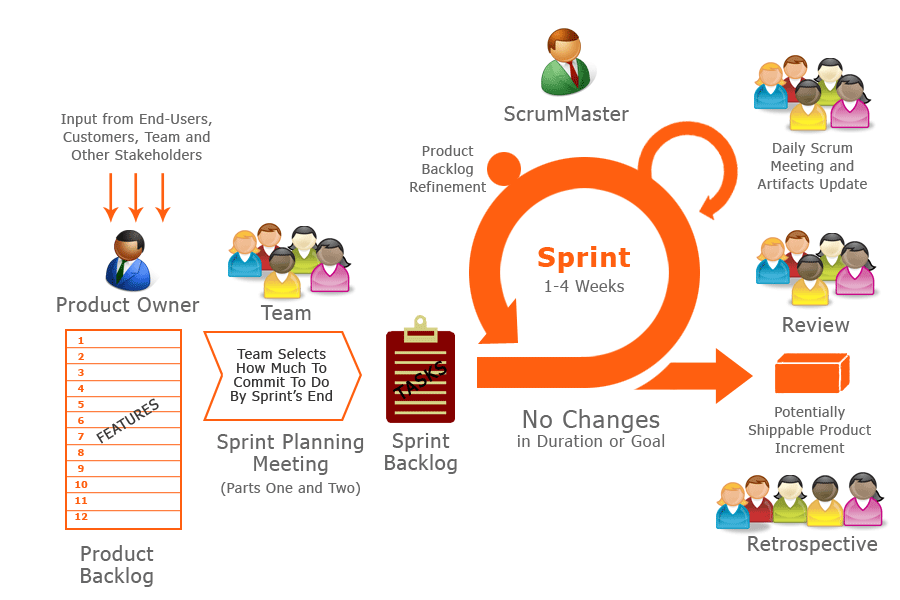
\includegraphics[width=0.9\columnwidth]{dig-scrum.png} 
    \caption{Diagramma flusso Scrum}
    \label{fig:scrum} 
\end{figure}             % Processi
% !TEX encoding = UTF-8
% !TEX TS-program = pdflatex
% !TEX root = ../tesi.tex

%**************************************************************
\chapter{Descrizione dello stage}
\label{cap:descrizione-stage}
%**************************************************************

\intro{Breve introduzione al capitolo}\\

%**************************************************************
\section{Introduzione al progetto}
\subsection{Descrizione del prodotto}
Il progetto ha come scopo la creazione di un’estensione del servizio MonoKee basato su \gls{blockchaing}. L’estensione offre un sistema di Identity Access Management (IAM) composto da quattro principali fattori:
    \begin{itemize}
        \item \textbf{Identity Wallet} (IW);
        \item \textbf{Service Provider} (SP);
        \item \textbf{Identity Trust Fabric} (ITF);
        \item \textbf{Trusted Third Party} (TTP);
    \end{itemize} 
In sintesi l’estensione dovrà operare al fine di fornire la possibilità ad un utente di registrare e gestire la propria identità autonomamente tramite l’IW e mandare i propri dati (PII) all’ITF, il quale custodirà la sua identità e farà da garante per le asserzioni proveniente dai TTP. Inoltre il SP dovrà essere in grado con le informazioni provenienti da IW e ITF di verificare o meno l’accesso ai propri servizi.
L'immagine in figura \ref{fig:diag-mod} dovrebbe chiarificare i vari componenti in gioco.
\begin{figure}[!h]
    \centering
    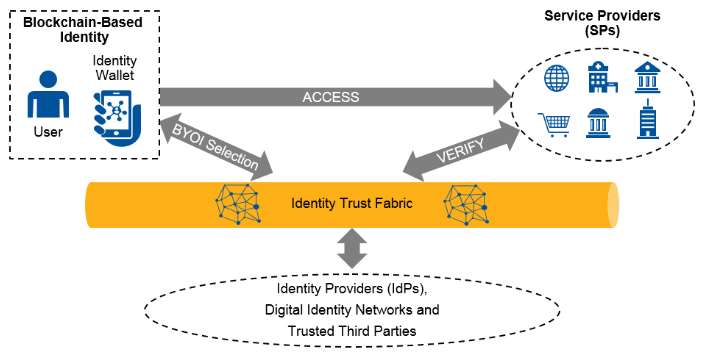
\includegraphics[width=0.9\columnwidth]{diagrammaComponenti.png} 
    \caption{Diagramma Moduli}
    \label{fig:diag-mod} 
\end{figure}
%**************************************************************
\section{Studio Tecnologico Identity Trust Fabric}

\subsection{Sintesi dello studio tecnologico}
Il capitolo procede descrivendo le caratteristiche del prodotto MonoKee e di come la tecnologia \gls{blockchaing} si possa collocare in tale contesto; vengono poi trattati i principali strumenti e librerie disponibili per sviluppare in Ethereum. L’analisi si conclude facendo emergere come un utilizzo di Ethereum sia possibile, ma non consigliato; le ragioni sono prettamente legate alla scalabilità del sistema. Per ragioni di facilità di sviluppo e di time to market si è ritenuto ad ogni modo di adottare la scelta di Ethereum come base del componente ITF.

\subsection{ITF – Identity Trust Fabric}
Sulla base di un primo studio di fattibilità l’unico componente coinvolto nell’uso \gls{blockchaing} è l’Identity Trust Fabric. La sua principale funzione è quella di poter permettere ai vari Service Provider aderenti al servizio di poter verificare le informazioni rilasciate dai vari utenti tramite l’utilizzo del loro personale Identity Wallet (IW). Il componente mantiene al suo interno l’hash della chiave pubblica degli utenti (che rappresenta la loro identità) e le asserzioni fornite dai vari IW che possono essere potenzialmente certificate da una TTP (tramite una firma con la loro chiave privata). Le asserzioni devono poter essere modificate o eliminate in ogni momento, naturalmente ogni alterazione deve essere di volta in volta certificata nuovamente. Anche da parte del TTP ci dev’essere la possibilità di revocare la certificazione di un’asserzione. 
Secondo lo studio Gartner in nota \footcite{farah:The-Dawn-of-Decentralized-Identity} una buona implementazione di una ITF deve possedere le seguenti caratteristiche:
\begin{itemize}
    \item \textbf{Fiducia}: il contenuto presente nella ITF deve essere solo quello autorizzato e non ci devono poter essere manomissioni malevoli da parte degli utilizzatori della rete. Ogni componente deve potere aver fiducia nella veridicità dei dati.
    \item \textbf{Garanzia}: le regole logiche della ITF non devono poter essere manomesse. Deve essere possibile applicare le varie policy aziendali in ambito di gestione dei rischi.
    \item \textbf{Tracciabilità}: ogni informazione e cambio di stato relativo alle identità e alle asserzioni deve poter essere tracciato e verificabile sia in termini cronologici sia in termini di provenienza. 
    \item \textbf{Sicurezza}: intesa come CIA. L’ITF deve rispettare i vincoli di confidenzialità, inalterabilità e disponibilità delle informazioni dentro lei contenute.
    \item \textbf{Scalabilità}: l’ITF deve fornire un elevato grado di scalabilità soprattutto in un’ottica in cui il prodotto potrebbe essere reso disponibile ad un uso Consumer.
    \item \textbf{Efficienza}: il funzionamento dell’ITF deve richiedere la minima quantità di risorse possibili.
\end{itemize}

\subsection{Introduzione alla tecnologia \gls{blockchaing}}
Al fine di rendere più consapevoli ai lettori le seguenti trattazioni si procede ad una esposizione ad alto livello dei principali concetti inerenti alla blockchain.
\emph{Blockchain} è comunenente definita come una base di dati distribuita composta da una serie di blocchi i quali possono contenere insiemi di dati o codice. In entrambi i casi questi sono temporalmente firmati.
Ogni blocco contiene l'hash del blocco precedente. In questo modo si crea una sorta di collegamento fra i blocchi che forma una catena, la cosidetta \emph{blockchain}. In questa catena solo il blocco successore può collegarsi al predecessore

Consideriamo, quindi, \emph{blockchain} una qualsiasi piattaforma informatica \textbf{distribuita} che possiede almeno le seguenti tre caratteristiche tecniche al fine di fornire un registro a prova di manomissioni: 
\begin{itemize}
    \item uso di funzioni crittografiche di \gls{hashg};
    \item uso di strutture dati con \emph{hash pointer};
    \item uso di protocolli di consenso distribuito.
\end{itemize}

L'uso di funzioni di hash e di strutture dati basate su \emph{hash pointers} conferisco a questa particolare tecnologia le sue peculiari caratteristiche di immutabilità dei dati e di conseguenza la rendono abile a fornire un registro a prova di manomissioni. Un registro con queste caratteristiche costituisce a sua volta un'affidabile struttura dati in grado di immaganizzare qualsiasi tipo di dato. Questo rende anche possibile l'aggiungere di nuovi dati in coda al registro. 

Chiunque tenti di modificare un qualsiasi punto della blockchain, renderà in questo modo l'\emph{hash pointers} presente nel nodo successore errato. Se costudiamo la testa della catena, anche se l'attacante modifica i nodi successivi della catena in modo da renderli consistenti all'alterazione che ha cercato di intrurre, saremmo comunque in grado di identificare la manomissione verificando la corretezza del puntatore di testa.

Altra caratteristica fondamentale è l'uso di un alogoritmo di consenso distribuito, questo rende possibile lo sviluppo di applicazioni distribuite; le cosidette \emph{dapp}. Una \emph{dapp} imaggazzina i propri dati e i propri registri delle operazioni in una \emph{blockchain} in modo di evitare qualsiasi qualsiasi punto di vulnerabiltà singolo (\emph{single point of failure}). Un ottimo esempio di \emph{dapp} può essere una qualsiasi cripto-moneta.

\subsubsection{Funzione crittografica di hash}
Una funzione di hash è una funzione matematica che converte un input di qualsiasi lunghezza in un output di lunghezza definita efficacemente. Una funzione di hash per essere considerata sicura deve possedere almeno le seguenti caratteristiche:
\begin{itemize}
    \item essere invertibile;
    \item resistente alle collisioni;
    \item essere puzzle-friendly.
\end{itemize}
Essere invertibile significa che non ci dev'essere nessun algoritmo tecnicamente fattibile in grado di identificare l'input dall'output.
Essere resistente alle collisioni significa che non ci dev'essere nessuna tecnica in grado di individuare casi in cui a due input differenti corrispenda uno stesso output. Questo non inplica che la funzione debba essere iniettiva.
Essere puzzle-friendly significa che la tecniche più facile per inveritire una funzione di hash è quella del \emph{brute forcing}. Questa ultima caratteristicha risulta fondamentale nel contesto dell'algoritmo di consenso.

\subsubsection{Puzzle di ricerca}
Il puzzle di ricerca consiste in un problema matematico che per essere risolto necessità di una ricerca della soluzione in un vasto dominio. Si dice che un puzzle di ricerca è puzzle-friendly quando non è presente nessuna strategia migliore rispetto al provare valori casuali. Questo tipo di problemi computazionali vengono adottati da alcune \emph{blockchain} come base delle cosidette \gls{powg}, particolari algoritmi di consenso nei quali i vari nodi della rete competono per la risoluzione del problema. L'attuazione di questo algoritmo rende possibile la decentralizzazione. Nelle \emph{blockchain} basate su \gls{powg} il nodo che riesce a risolvere il puzzle per primo viene riconosciuto come prossimo nodo che inserirà un blocco nella catena 

\subsubsection{Commitment}
Un \emph{commitment} è l'equivalente digitale di leggere un valore, sigillarlo in una busta e poi metterla in un luogo sicuro. Il valore prelevato rimane segreto agli altri nodi fino a che il nodo che ha effettuato il \emph{commitement} non decida di rivelarlo. Le due funzioni che rendona questo possibile sono il \textbf{commit} e la \textbf{verify}.

Il \emph{commit} è una funzione che prende un messaggio e un numero randomico secrete ( \gls{nonceg}\glsfirstoccur) come input e ritorna un  \emph{commitment}.

La \emph{verify} è una funzione che prende \emph{commitment}, \gls{nonceg} e messaggio come input. Restituisce \emph{true} in caso la funzione di \emph{commit} con input il messaggio e il nonce passati abbia un output corrispondente al commitment fornito. In tutti gli altri casi ritorna \emph{false}.

Per usare questo schema abbiamo come primo passo quello di generare un numero randomico in qualità di nonce. Poi ci usando la funzione \emph{commit} pubblichiamo un \emph{commitment} usando il nonce appena generato. In un secondo momento, quando vogliamo rivelare il valore commitato in precedenza, pubblicheremo il nonce e il messaggio usati con la funzione di \emph{commit}. Una terza parte potrà poi essere in grado di verificare il messaggio tramite l'uso della funzione \emph{verify}.
Questa particolare tecnica risulta particolarmente utile al fine di immaganizzare le identità o attributi su di essa all'interno della \emph{blockchain}. Un \emph{commitment} per essere tale deve nascondere le informazioni. Questa significa che non potranno più essere alterate. 

\subsubsection{Strutture dati con hash pointer}
Un \emph{hash pointer} è un puntatore verso il posto dove un dato è contenuto, unito al valore del dato sotto forma di hash. A differenza di un normale puntatore che è solo in grado di fornirti un modo per ottenere l'informazione, un \emph{hash pointer} permette anche di essere in grado di capire se il particolare dato è stato alterato dalla creazione del puntatore. Questo particolare puntato può essere usato per la creazione di tipiche strutture dati concatenate, quali liste e alberi. La \emph{blockchain} è una lista concatenata(\emph{linked list}) costruita usando \emph{hash pointer} in vece ai classici puntatori. In una \emph{blockchain}, ogni blocco non solo ci dice dove si trova il blocco precedente, ma ci fornisce anche il valore dell'hash di questo blocco permettendoci quindi di poter verificare qualsiasi alterazione. Le particolari caratteristiche degli \emph{hasp pointer} usati ci permette di verificare l'intera catena a partire dal blocco di testa del quale ci dobbiamo fidare. 
Un'immagine esplicativa di quanto appena detto è presente in figura \ref{fig:linked-list}

\begin{figure}[!h]
    \centering
    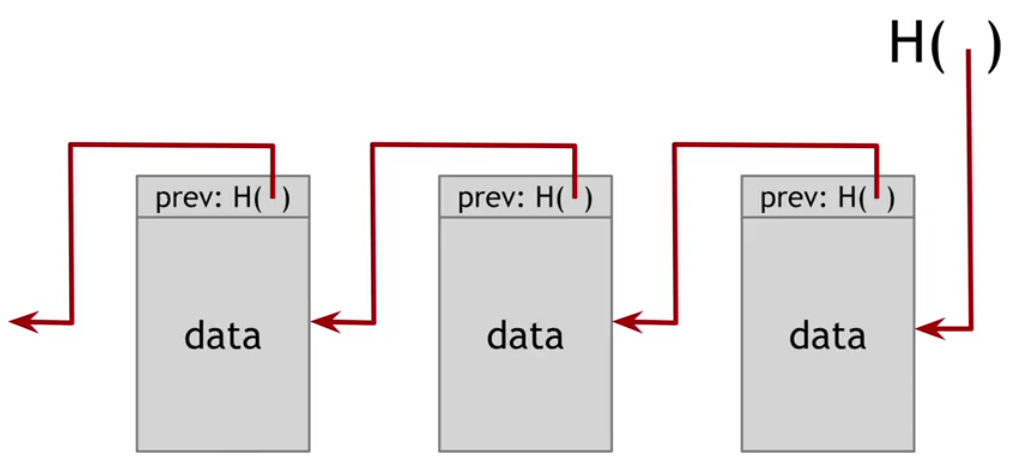
\includegraphics[width=0.9\columnwidth]{linked-list.png}
    \caption{Lista concatenato con \emph{hash pointer}}
    \label{fig:linked-list} 
\end{figure}

\subsubsection{Albero di Merkle}
Comunamente le principali \emph{blockchain} fanno uso di una particolare struttura dati per immagazzinare la loro componente di dati, l'albero di Merkle. L'albero di Merkle è un albero binario che usa \emph{hash pointer} in sostituzione dei classici puntatori. I record in quest'albero sono strutturati in coppie, e i loro hash conservati un livello superiore. Questa definizione si applica ad ogni livello del nodo fino al raggiungimento della radice. Le foglie rappresentano i dati. La figura \ref{fig:markle-tree} dovrebbe esporre con chiarezza il concetto.

\begin{figure}[!h]
    \centering
    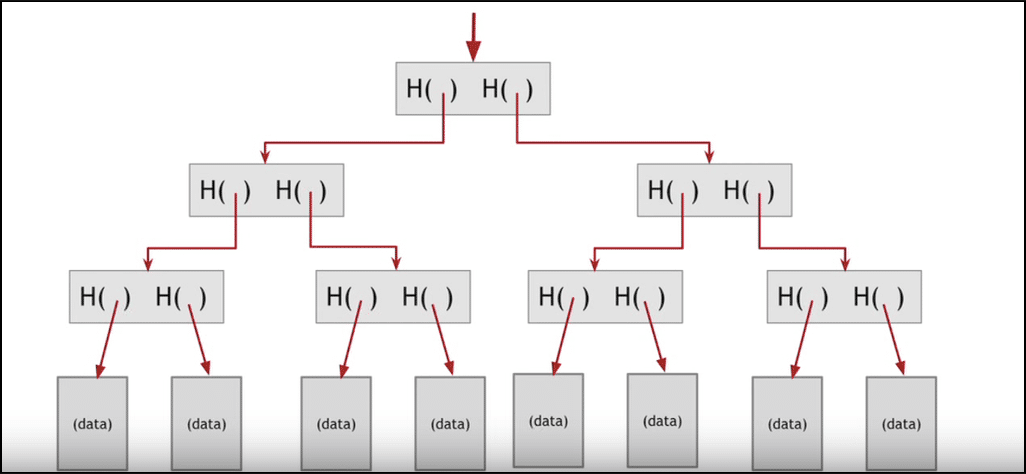
\includegraphics[width=0.9\columnwidth]{merkle-tree.png}
    \caption{Albero di Merkle}
    \label{fig:merkle-tree} 
\end{figure}

In caso di alterazioni in un qualsiasi nodo dell'albero queste sarebbero rilevabile in quanto causerebbero delle incoerenze nei puntatori presenti nei nodi al livello superiore. L'uso di questa struttura nel contesto di una \emph{blockchain} semplifica la verifica dell'attribuzione dei blocchi e permette di dover conservare solo la radice nel blocco di testa.

\subsubsection{Algoritmo di consenso}
Abbiamo visto come l'uso di funzioni di hash e di strutture dati particolari rendono la \emph{blockchain} un'affidabile e verificabile base di dati centralizzata. Uno dei principali fattori di successo della tecnologia è stata però la natura decentralizzata di essa. Questa è possibile grazie all'uso di molteplici nodi in sostituzione ad un server centralizzato. La presenza di un algoritmo di consenso rende possibile ai vari nodi partecipanti accordarsi su cosa debba essere scritto o meno nella catena. Assumento che i vari nodi (anche malevoli) ricevano un input valido l'algoritmo di consenso assicura le seguenti proprietà:
\begin{itemize}
    \item l'algoritmo termina quando tutti i nodi onesti sono in accordo sul valore;
    \item l'algoritmo assicura che il valore è stato prodotto da un nodo onesto. 
\end{itemize}

In questo caso, un nodo onesto viene scelto per inserire il proprio blocco in cosa alla catena. In questo modo, l'algoritmo permette al sistema di generare fiducia in un contesto in cui nessun nodo si fida dell'altro.

Tipicamente in una \emph{blockchain} avvengono le seguenti operazioni. A intervalli regolari, ogni nodo propone le proprie transazioni in sospeso per essere inserite come prossimo blocco. Successivamente si attua l'algoritmo di consenso in cui ogni nodo proprone come input il blocco che intendono inserire. Alcuni nodi potrebbero essere malevoli e inserire transazioni non valide nei proprio blocco di input, ma possiamo assumere che gli altri nodi sono onesto. Se l'algoritmo di consenso ha successo viene selezionato il blocco da inserire in coda. Nessuno decide quale sarà il prossimo nodo ad essere inserito nella blockchain.

C'è comunque da ricordare che la presente è una trattazione ad alto livello, e quindi non verranno presentati particolari algoritmi di consenso. Mi limito quindi a presentare le principali carattestiche che questo deve avere:
\begin{itemize}
    \item equità;
    \item velocità;
    \item dimostrabilità;
    \item resistenze al problema dei generali bizantini;
    \item efficente;
    \item resistente ad attacchi Dos e DDos.
\end{itemize}

\subsection{Permissionless e Permissioned \gls{blockchaing}}
Al fine di poter valutare la fattibilità dell’utilizzo di Ethereum quale \gls{blockchaing} sottostante all’ITF è necessario avere in mente le due principali categorie di \gls{blockchaing}: \textbf{permissionless} e \textbf{permissioned}.

\subsubsection{Permissioned \gls{blockchaing}}
Una permissioned \gls{blockchaing} pone dei vincoli sulla partecipazione alla rete. Soli i nodi autorizzati possono partecipare all’algoritmo di consenso dei blocchi. Le autorizzazioni possono essere date singolarmente, quindi i vari nodi possono avere o meno le seguenti possibilità:
\begin{itemize}
    \item lettura dei blocchi;
    \item scrittura dei blocchi;
    \item esecuzione di codice (se prevista dalla \gls{blockchaing});
    \item verifica dei nodi.
\end{itemize}

\subsubsection{Permissionless blockchaing}
Una permissionless \gls{blockchaing} è una rete in cui qualsiasi nodo può partecipare al processo di verifica dei blocchi. Ogni nodo ha tutte le precedenti quattro proprietà.

\paragraph{Ethereum}
Ethereum è una piattaforma decentralizzata pubblica ed open-source basata sulla creazione di \gls{SmartContractg}. Permette la creazione di applicazioni che operano su \gls{blockchaing} in modo che non ci sia alcuna possibilità di downtime, censura, frodi o interferenze da terze parti. Rappresenta una dei principali esempi di rete permissionless.
La piattaforma è stata rilasciata nel corso del 2014 ed è mantenuta dalla Ethereum Foundation. Questo fa di Ethereum una delle più longeve \gls{blockchaing} disponibili. Ciò comporta la presenza di una documentazione abbastanza nutrita rispetto ai competitor e di un buon numero di strumenti già disponibili. 
L’elevata popolarità della tecnologia e alcune sue caratteristiche non presenti nei competitor, ha fatto sì che una notevole quantità di sviluppatori abbiano deciso di utilizzarla. Il sito \footnote{site:state-dapps} mantiene una vetrina di oltre milleseicento esempi. Sono presenti tutte le più significative applicazioni ora in produzione. Si fa notare che molte delle quali sono state le fonti dei più diffusi pattern Ethereum.

\paragraph{Programmare SmartContract}
Solidity è il principale linguaggio di programmazione usato per scrivere \gls{SmartContractg}. Nonostante sia presente un’implementazione basata su Go, questa è ancora acerba e non largamente utilizzata. Per questo motivo questa implementazione non verrà trattata in questo documento.
Solidity è un linguaggio di programmazione ad oggetti ad alto livello. Il suo sviluppo è stato fortemente influenzato da linguaggi quali C++, Python e Javascript. Gli SmartContract così scritti vengono poi trasformati in bytecode e quest’ultimo viene eseguito dall’Ethereum Virtual Machina (EVM).
Il linguaggio seppur non completamente maturo offre la maggior parte delle caratteristiche tipiche di un linguaggio ad oggetti. Infatti Solidity è fortemente tipato, supporta l’ereditarietà, librerie esterne e tipi definiti dall’utente. A sottolineare la bontà del linguaggio si evidenzia come in Solidity sia presente il concetto di interfaccia, caratteristica non presente in linguaggi ben più longevi. 
Queste caratteristiche rappresentano un notevole vantaggio per Ethereum rispetto ai diretti competitor, i quali spesso utilizzano linguaggi acerbi e/o a basso livello. Si ritiene che un linguaggio con le precedentemente descritte caratteristiche sia fondamentale per la buona riuscita del progetto, soprattutto in un’ottica di manutenibilità e estendibilità.
\paragraph{Breve nota sull'applicabilità dei pattern}
Nonostante il linguaggio permetta l’applicabilità dei più diffusi pattern si vuole far notare come nel contesto di una blockchain Permissionless questi risultino spesso controproducenti. 
Durante la progettazione e l’applicazione dei pattern vanno sempre ricordati i seguenti punti:
\begin{itemize}
    \item l’esecuzione di un metodo che modifica la blockchain si paga in base al lavoro che viene effettivamente svolto;
    \item complessità lineari portano a costi difficilmente accettabili;
    \item plugin come Metamask calcolano il massimo costo possibile di una transazione, in caso il credito non sia sufficiente la transazione fallisce. Quindi un ciclo for su una lista di un elemento viene stimato presupponendo che la lista sia completamente piena;
    \item la velocità di esecuzione varia in base alla somma pagata per questa, anche con somme estremamente alte o su reti locali i tempi potrebbero essere considerati non giustificabili per la maggior parte degli utenti;
    \item ogni oggetto e campo dato si paga in base al loro spazio occupato;
    \item il costo della moneta e quindi delle transazioni è fortemente variabile. Approcci un giorno economici possono diventare economicamente insostenibili a distanza di giorni.
\end{itemize}
A seguito dei precedenti punti dovrebbe risultare più evidente come pattern che prevedono alta complessità temporale e spaziale siano inaccettabili su una rete Ethereum. Ad esempio i pattern Command e Decorator risultano difficilmente giustificabili.
Sono invece presenti pattern pensati appositamente per Ethereum, questi sono presenti nella documentazione ufficiale Solidity \footcite{site:solidity-documentation}. Particolarmente utili al contesto del progetto in esame ritengo possano utili i seguenti pattern: 
\begin{itemize}
    \item Owner Pattern;
    \item Vote Pattern 
    \item WhiteList Pattern.
\end{itemize}

\paragraph{Complessità e pratiche non convenzionali}
I punti precedentemente stilati nel paragrafo sull’applicabilità dei pattern portano anche delle notevoli differenze in termini di pratiche di stile di programmazione. Tra queste riporto:
\begin{itemize}
    \item l’uso di liste e array sono fortemente sconsigliato, vanno preferite struttura con accesso costante. Solidity fornisce il tipo mapping;
    \item la creazione di oggetti (in termini Solidity contratti) ha un costo notevole. Una buona pratica è quella di utilizzare ADT (Abstract Data Type) differenti come le strutture;
    \item cicli for che portano complessità lineare dovrebbero essere evitati, elaborazioni di questo tipo dovrebbero essere affidate a server esterni o a livello client-side;
    \item l’utilizzo dei puntatori (in Solidity address) nasconde completamente il tipo dell’oggetto puntato rendendo vano il controllo dei tipi. Andrebbe evitato il più possibile.
\end{itemize}
Si fa notare come in particolare l’ultimo punto degeneri completamente il concetto di programmazione ad alto livello.

\paragraph{Strumenti}
Come già citato la relativa maturità della tecnologia ha portato alla creazione di alcuni utili strumenti. 
\begin{itemize}
    \item \textbf{Truffle}: è una suite di development e testing. Permette di compilare, buildare ed effettuare la migrazione degli SmartContract. Inoltre ha funzioni di debugging e di scripting. La suite offre la possibilità di effettuare test degli SmartContract sia in Javascript (con l’utilizzo di Chai), sia in Solidity. Si riporta di seguito il sito del progetto: \cite{site:truffle}.
    \item \textbf{Ganache}: è uno strumento rapido che permette di creare e mantenere in locale una rete blockchain Ethereum personale. Può essere usata per eseguire test, eseguire comandi e per operazioni di controllo dello stato mentre il codice esegue. Si riporta di seguito il sito del progetto: \cite{site:ganache}.
    \item \textbf{Mist}: è un browser sviluppato direttamente dal team Ethereum in grado di operare transazioni direttamente nella blockchain senza la necessità di possedere un intero nodo. È estremamente immaturo e non utilizzabile in produzione. Si riporta di seguito il sito del progetto: \cite{site:mist}.
    \item \textbf{Parity}: è un client Ethereum che permette di operare sulla rete senza necessità di possedere un intero nodo. Questa soluzione a differenza di Mist dovrebbe risultare più facilmente integrabile nel prodotto senza che l’utente ne abbi consapevolezza. Si riporta di seguito il sito del progetto: \cite{site:parity} .
    \item \textbf{Metamask}: è uno plugin disponibile per i browser Chrome, Firefox, e Opera che permette di interfacciarsi alla rete Ethereum senza la necessità di eseguire in intero nodo della rete. Il plugin include un wallet con cui l’utente può inserire il proprio account tramite la chiave privata. Una volta inserito l’account il plugin farà da tramite tra l’applicazione e la rete.
    Metamask è utilizzato dalla maggioranza delle applicazioni Ethereum presenti on line, questo però rappresenterebbe un componente esterno compatibile con pochi browser desktop. Si riporta di seguito il sito del progetto: \cite{site:metamask} .
    \item \textbf{Status}: è un progetto che propone una serie di \gls{apig} che permettono di sviluppare un’applicazione mobile nativa operante direttamente su blockchain senza la necessità di possedere un intero nodo. Il sito del progetto propone una serie di applicazioni che utilizzano Status tuttavia nessuna di queste applicazioni risulta attualmente rilasciate in nessuno store. Status risulta in early access ed è disponibile per Android e iOS. Il sito del progetto è il seguente: \cite{site:status}.
    \item \textbf{Microsoft Azure}: “Ethereum Blockchain as a Service” è un servizio fornito da Microsoft e ConsenSys che permette di sviluppare a basso costo in un ambiente di dev/test/produzione. Permette di creare reti private, pubbliche e di consorzio. Queste reti saranno poi accessibili attraverso la rete privata Azure. Questa tecnologia rende facile l’integrazione con Cortana Analytics, Power BI, Azure Active Directory, O365 e CRMOL.
\end{itemize}

\paragraph{Valutazione applicabilità soluzione Ethereum}
Al fine di poter valutare correttamente da ogni punto di vista l’applicabilità di una soluzione basata su Ethereum quale base della componente ITF, si procede ad analizzare in maniera analitica le sei caratteristiche presentate nel capitolo ‘ITF – Identity Trust Fabric’.

\begin{itemize}
    \item \textbf{Fiducia} \\
    Questa caratteristica è ottenuta da Ethereum da una combinazione di diversi fattori quali:
    \begin{itemize}
        \item utilizzo di incentivi economici, il pagamento per effettuare operazioni;
        \item utilizzo di prove di interesse (Proof of Interest).
    \end{itemize}
    Le prove di interesse possono essere di due tipi:
    \begin{itemize}
        \item Proof of Stake, l’esibizione di un interesse;
        \item Proof of Work, l’uso di potenza di calcolo per risolvere un problema matematico.
        Queste metodologie fanno in modo che solo chi realmente interessato possa influenzare l’algoritmo di consenso dei blocchi. Questo rende minore la possibilità di un "51 percent attack" \footcite{site:51-attack}. C’è comunque da ricordare che un attacco di questo tipo e praticamente impossibile.
    \end{itemize}
    Per queste ragioni si ritiene una rete Ethereum sia completamente soddisfacente per quanto riguarda l’aspetto fiducia, al pari di una rete di tipo permissioned.
    \item \textbf{Garanzia}\\
    Lo studio\footcite{farah:The-Dawn-of-Decentralized-Identity} evidenzia come questo rappresenti un punto critico. Infatti riporta che il raggiungimento di questo obiettivo è fortemente condizionata dall’efficacia dell’algoritmo di consenso e dai nodi presenti nella rete. Lo studio prosegue facendo notare che la presenza di nodi malevoli, oltre che mettere a rischio l’algoritmo di consenso, può compromettere anche il corretto funzionamento dell’ITF. Infatti trattandosi di una blockchain pubblica ogni nodo è in grado di visionare il contenuto di ogni singolo contratto, inclusi i dati e i metodi presenti. Per quanto riguarda i dati questo potrebbe non essere un problema in quanto si può immagazzinare una versione codificata del dato. Per quanto riguarda i metodi questo non è possibile, questo potrebbe rendere in grado ad un attaccante di trovare eventuali bachi e criticità dell’ITF. Il servizio Azure potrebbe permette di creare reti private.
    \item \textbf{Tracciabilità}\\
    Lo studio Gartner\footcite{farah:The-Dawn-of-Decentralized-Identity} evidenzia come in una rete permissionless la tracciabilità temporale non sia possibile, in quanto in una rete distribuita ogni nodo può avere un concetto di tempo proprio. Questo però non risulta possibile in nessun approccia risolutivo all’ITF basato su blockchain. Infatti le reti permissioned applicano timestamp a livello di blocco e non di transazione, anche ammettendo che ci sia un concetto di tempo comune tra i nodi, le transizioni rimarrebbero temporalmente non tracciabili. La cosa potrebbe permettere ad un blocco di alterare l’ordine delle transazioni. 
    Questo problema in una rete permissioned può essere risolto creando blocchi immutabili e ogni volta si voglia fare una modifica si dovrà creare un nuovo blocco. In questo modo ci sarà solo una transazione di creazione blocco il cui timestamp coinciderà con il timestamp del blocco.
    Questo approccio in Ethereum rimane comunque impraticabile. Attualmente non sono note ulteriori tecniche per la tracciabilità temporale in Ethereum. Per questa ragione l’attribuzione di un riferimento temporale dovrà essere effettuato lato client, con i conseguenti limiti di sicurezza. 
    \item \textbf{Sicurezza}\\
    La confidenzialità dei dati anche se non presente nativamente in Ethereum e facilmente ottenibile immagazzinando nei contratti solo un hash dei dati.
    L’integrità dei dati invece è garantita dalla prova di lavoro che utilizza la blockchain come già ribadito nella sezione Fiducia.
    La disponibilità invece è garantita dalle caratteristiche di distribuzione di ogni blockchain.
    Un ulteriore punto di considerazione da fare è che chiunque ha la possibilità di vedere il contenuto di ogni SmartContract incluso il codice dei metodi. Questo come già detto può comportare la possibilità da parte di un attaccante di individuare eventuali errori logici. Ogni contratto dovrà comunicare con gli altri attraverso chiamate a metodi pubblici, in quanto non c’è in Ethereum nessun concetto di visibilità dei metodi di tipo protected o package. Questo rende possibile da parte di qualsiasi utente della rete di utilizzare questi metodi in maniera malevole. Questo tipo di problematica è facilmente superabile applicando i dovuti pattern Solidity quali WhiteList Pattern e Owner Pattern. L’applicazione dei pattern però comporterebbe un notevole aumento in termini di complessità e costo soprattutto in presenza di logiche di accesso variegate e dinamiche. Inoltre, in caso di liste di utenti autorizzati l'immagazzinazione di queste liste potrebbe risultare oneroso in termini di costi.
    \item \textbf{Scalabilità}\\
    Ethereum per poter applicare l’algoritmo del consenso fa utilizzo di una prova di lavoro. Questa deve essere fatta in occasione di ogni transazione. La prova consiste nella risoluzione di un problema crittografico la cui difficoltà è dinamica in base a diversi fattori della blockchain quali valore dell’Ether, numero di utenti, numero di transazioni, etc. Inoltre si nota come anche in lettura ci sia una lentezza che difficilmente potrebbe essere ritenuta accettabile da un utente medio. Per avere prova di questo fatto si può prendere in esame una qualsiasi Dapp presente al seguente link \footcite{site:state-dapps}. La questione pone anche limitazioni come già citato in termine di costo.
\end{itemize}
\subsection{Conclusioni}
Da quanto è emerso l’utilizzo della tecnologia Ethereum quale base dell’ITF pone una serie di vantaggi e svantaggi. Di seguito si propone una sintetica trattazione dei punti fondamentali, per maggiori dettagli si consiglia la lettura dell’intero documento.
I vantaggi sono:
\begin{itemize}
    \item Ethereum offre un linguaggio ad alto livello e ad oggetti a differenza di altri competitor;
    \item Ethereum offre una notevole maturità e anche un’ampia platea di strumenti, molti dei quali estremamente maturi e largamente utilizzati.
\end{itemize}
    
Gli svantaggi sono: 
\begin{itemize}
    \item Ethereum è una rete pubblica, non è possibile fare nessuna restrizione di privilegi sui nodi partecipanti alla rete. Questo potrebbe rappresentare un problema di sicurezza;
    \item la comunicazione verso dispositivi mobili non è verificabile da quest’ultimi, in quanto dovrebbe avvenire tramite comunicazione REST;
    \item sono presenti forte limitazioni in termini di costo e velocità, il sistema risulterebbe lento ed estremamente costoso. Ciò comporta notevoli problemi in termini di Scalabilità del servizio.
\end{itemize}
Si ritiene che un approccio basato sul Ethereum sull’ITF sia possibile, le eventuali criticità di sicurezza e fiducia verso i dispositivi mobili sono superabili con una buona progettazione. L’unico fattore veramente critico risulta la scalabilità del sistema. Quest’ultimo fatto a mio parere è sufficiente per ritenere Ethereum non adatto all’utilizzo soprattutto in un’ottica commerciale. Quindi se pure possibile, non si consiglia l’utilizzo di Ethereum. Per ragioni di facilità di sviluppo e di time to market si è ritenuto comunque di adottare la scelta di Ethereum come base del componente ITF.

%**************************************************************

\section{Studio di fattibilità Identity Wallet}
\subsection{Sintesi dello studio di fattibilità}
Lo studio inizia descrivendo come l’IW si cali in questo contesto. Si prosegue analizzando le alternative di sviluppo mobile e Desktop. A seguito di un’analisi dei possibili utenti emerge una netta preferenza per lo sviluppo mobile.
Vengono poi trattati i principali strumenti e librerie disponibili per lo sviluppo. Si ritiene di preferire uno sviluppo multi piattaforma, con target Android e iOS. L’analisi conclude facendo emergere una preferenza per il framework Xamarin.
\subsection{Descrizione componente Identity Wallet} 
Il progetto ha come scopo la creazione di un Identity Wallet (IW). L’applicativo si colloca nel contesto di un’estensione del servizio Monokee basato su blockchain. L’estensione offre un sistema di \gls{iamg} composto da quattro principali fattori:
\begin{itemize}
    \item Identity Wallet (IW)
    \item Service Provider (SP)
    \item Identity Trust Fabric (ITF)
    \item Trusted Third Party (TTP)
\end{itemize}
    
In sintesi l’estensione dovrà operare al fine di fornire la possibilità ad un utente di registrare e gestire la propria identità automatamente tramite l’IW, mandare i propri dati (IPP) all’ITF la quale custodirà la sua identità e farà da garante per le asserzioni proveniente dai TTP. Inoltre il SP dovrà essere in grado con le informazioni provenienti da IW e ITF di garantire o meno l’accesso ai propri servizi.
Il software IW, più dettagliatamente, dovrà assolvere ai seguenti compiti:
nell’ambito della registrazione di un utente il Wallet deve:
\begin{itemize}
    \item generare e immaganizzare in locale una chiave pubblica;
    \item generare e immaganizzare in locale una chiave private;
    \item creare l’hash della chiave la chiave pubblica e inviare l’hash all’ITF;
    \item incrementare le informazioni (PII) relative alle identità che il Wallet gestisce.
\end{itemize}
Nell’ambito della presentazione dei dati ad un Service Provider deve:
\begin{itemize}
    \item invio della chiave pubblica al service provider;
    \item invio di un puntatore all’hash della chiave pubblica interna al ITF;
    \item invio di altre informazioni utili presenti nel ITF;
    \item gestire ulteriori layer di sicurezza, quali impronta digitale, QR code, autentificazione multi fattore)
\end{itemize}
nell’ambito della richiesta di accesso ad un servizio deve:
\begin{itemize}
    \item inviare una richiesta di accesso ad un servizio con i dati relativi all’identità al Service Provider;
    \item attendere la risposta del Service Provider.
\end{itemize}

\subsection{Studio del dominio}
\subsubsection{Dominio Applicativo}
L’applicativo IW dovrà essere usato in un contesto prevalentemente lavorativo. Non si escludono però ulteriori applicazione future in ambito Consumer. In ogni caso il software dovrà poter essere usato da utenti senza specifiche conoscenze informatiche e con minimo training tecnologico. Dato il contesto applicativo il software dovrà essere il più accessibile e semplice possibile. Per queste ragioni si pensa ad un suo utilizzo prevalentemente in ambito mobile, anche se non si esclude a priori la possibilità di una versione Desktop. L’applicativo mobile deve essere disponibile per la più ampia gamma di utenti possibili.
\subsubsection{Dominio Tecnologico}
Un eventuale applicativo Desktop ha un’elevata probabilità di non rientrare dentro i tempi dello stage, per questo si ritiene di non tenerlo in considerazione. L’applicativo quindi dovrà essere fruibile tramite un’applicazione mobile multipiattaforma sviluppabile entro i limiti temporali della durata dello stage. 
Per queste ragioni lo studio del dominio tecnologico si incentrerà principalmente su tecnologie multi piattaforma mobili. Verrà comunque tenuto in considerazione anche lo sviluppo nativo.
\paragraph{Studio diffussione sistemi operativi mobili}
Procedo di seguito ad un’analisi sulla diffusione dei vari sistemi operativi mobili.
I dati in figura ~\ref{fig:diff-os-mob} riportati provengono da Kantar \footcite{site:kantar-study} società di analisi inglese e fanno riferimento al trimestre che va da novembre 2016 a gennaio 2017.
\begin{figure}[!h] 
    \centering
    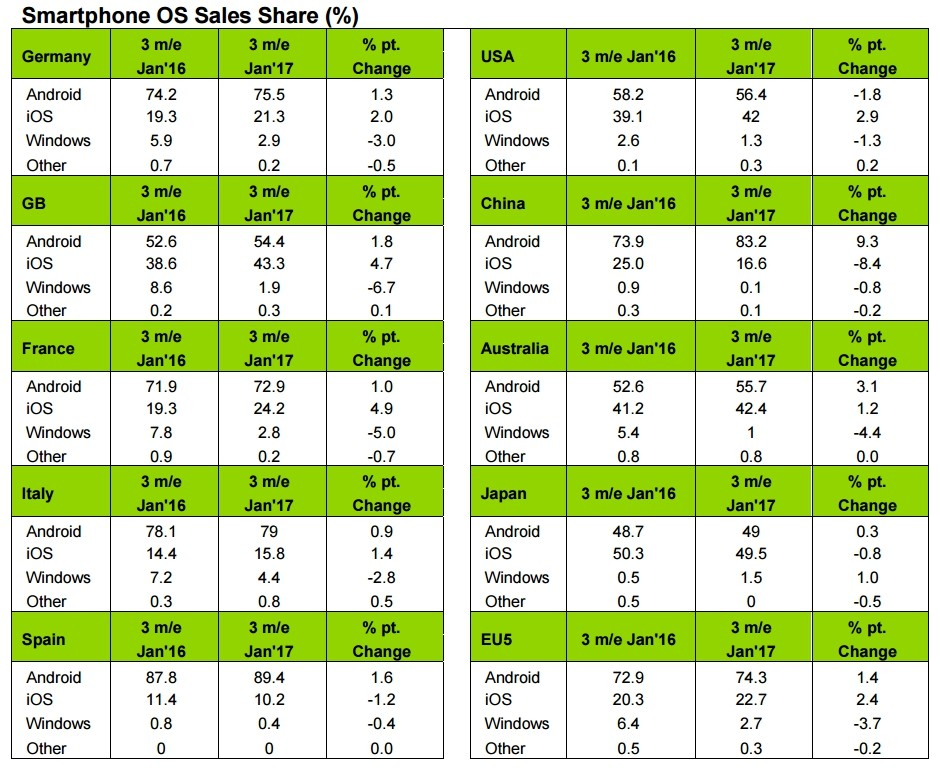
\includegraphics[width=0.9\columnwidth]{diff-os-mob.png} 
    \caption{Diffuzione sistemi mobili}
    \label{fig:diff-os-mob} 
\end{figure}
Da come si può evincere dai dati, Android, iOS, Windows Phone rappresentano, in questa sequenza ed in ogni mercato, i sistemi più diffusi. I restanti sistemi non raggiungono cifre significative. Ponendo maggiore attenzione ai primi tre sistemi si nota come Android nell’area EU5 rappresenti i tre quarti del mercato. In Giappone, Stati Uniti, Australia e Gran Bretagna invece la situazione risulta più bilanciata con una sostanziale parità. Windows Phone in ogni mercato si pone in terza posizione con percentuali che non superano mai l’otto percento. Individuando nell’area EU5 il principale mercato per MonoKee si ritiene che il prodotto IW debba essere sviluppato per i sistemi Android e iOS, dando la precedenza al primo. Non si ritiene necessario lo sviluppo di un’applicazione Windows Phone in quanto difficilmente attuabile nei tempi dello stage. 
\paragraph{Tecnologie per lo sviluppo}
Segue un approfondimento relativo alle potenziali tecnologie con cui sviluppare l’IW. Data la necessità di sviluppare sia per Android, che per iOS l’analisi si concentrerà principalmente su framework multi piattaforma senza comunque ignorare la possibilità di sviluppi nativi.
\paragraph{Sviluppo multipiattaforma}
Tra le principali alternati multi piattaforma si ritengono particolarmente interessanti le seguenti:
\begin{itemize}
    \item React Native;
    \item Cordova;
    \item Xamarin;
\end{itemize}
Segue un’analitica descrizione dei vari framework.

\textbf{React Native}: è un framework di sviluppo mobile derivato da React. Il progetto e sviluppato e mantenuto da Facebook. React Native si focalizza nello sviluppo di UI tramite componenti scritti in JavaScript, su un approccio funzionale e flusso di dati unidirezionale.  A differenza di React, React Native non manipola il DOM del browser, ma una struttura diversa. I componenti non vengono scritti a partire da elementi HTML o simili (i.e. Bootstrap o Grommet), ma bensì a partire da un set di componenti base presenti nella libreria. La libreria permette di sviluppare applicazioni per iOS e Android.

\textbf{Cordova}: è un framework open-source per lo sviluppo di applicazione mobili che propone un approccio ibrido e non nativo. Permette di usare tecnologie web ampiamente utilizzate, quali HTML5, CSS3, Javascript, per la codifica. Il software così prodotto verrà eseguito in appositi wrapper diversi per ogni piattaforma, quindi in maniera non nativa. Il framework è sviluppato da Apache ed ormai ha raggiunto un elevato grado di maturità. Rappresenta uno dei primi framework per lo sviluppo multi piattaforma.

\textbf{Xamarin}: è un framework per lo sviluppo di applicazioni native e multi piattaforma con C Sharp. Il framework si basa sul progetto open source Mono e offre pieno supporto non solo alle piattaforme Android e iOS ma anche a Windows Phone. La possibilità di sviluppare anche per Windows Phone potrebbe risultare un punto a favore rispetto agli altri framework. Xamarin si compone di tre componenti principali: Xamarin.Android, Xamarin.iOS, Xamarin.Forms. L’ultimo componente si pone come strumento completamento neutro rispetto alla piattaforma. Grazie a queste componenti è possibile gestire in C Sharp tutte le caratteristiche di Android, iOS e Windows Phone.
\medskip

 La tabella \ref{tab:comp-framework} riassume quanto appena detto.
\begin{table}[!h] %
    \caption{Tabella comparivi framework sviluppo applicazioni mobili}
    \label{tab:comp-framework}
    \begin{tabularx}{\textwidth}{llll}
    \hline
    \textbf{Framework} & \textbf{Approccio} & \textbf{Piattaforme supportate} &\textbf{Linguaggio}\\
    \hline
    React Native   & Nativo & iOS, Android & Javascript\\
    \hline
    Cordova   & Ibrido & iOS, Android & HTML5, CSS3, Javascript\\
    \hline
    Xamarin   & Nativo & iOS, Android, WP & C Sharp\\
    \hline
    \end{tabularx}
    \end{table}%
Data l’impossibilità degli approcci ibridi, quali Cordova, di sfruttare a pieno le caratteristiche tipiche delle diverse piattaforme mobili si ritiene di scartare questo tipo di soluzioni.
Inoltre si evidenziano difetti come una mancata o incompleta integrazione dell’aspetto grafico con la specifica piattaforma e una maggiore lentezza nell’esecuzione e accesso alle risorse locali.
Per queste ragione si ritiene più opportuno l’utilizzo di un framework che permetta di scrivere applicazioni in maniera nativa. 
Richiudendo la visione ai soli approcci nativi, Xamarin rispetto a React Native lascia aperte le porte ad una eventuale applicativo Windows Phone. Inoltre utilizza C Sharp un linguaggio che rispetto a Javascript fornisce una tipizzazione forte e caratteristiche più orientate agli oggetti. Per queste ragioni si consiglia l’utilizzo di Xamarin o React Native con la preferenza per il primo.
\paragraph{Sviluppo Nativo}
Un’applicazione nativa è un’applicazione mobile sviluppata interamente nel linguaggio del dispositivo sul quale vengono eseguite. Quindi stiamo parlando di Java per Android e Swift o Object-C per iOS. Il loro utilizzo presenta diversi vantaggi rispetto allo sviluppo multi piattaforma:
\begin{itemize}
    \item interazione con tutte le caratteristiche del dispositivo consentendo l’utilizzo al 100\%;
    \item maggiore velocità offrendo quindi una User Experience di più alto livello;
    \item facilità di integrazione di terze parti tramite utilizzo di SDK ufficiali. 
\end{itemize}
Il primo punto non dovrebbe rappresentare un plus in quanto non si ritiene che l’IW debba usufruire di feature particolari dei dispositivi. 
È da notare che uno sviluppo nativo richiede il doppio delle risorse necessarie in quanto prevede lo sviluppo di due applicazione completamente diverse (Android e iOS), con framework e quindi architetture potenzialmente diverse. 
Riassumendo, dato che: 
\begin{itemize}
    \item l’applicativo che si dovrà sviluppare non prevede particolari requisiti prestazionali;
    \item l’alto costo in termini orari di sviluppare soluzioni differenti ha una forte probabilità di non rientrare nei tempi previsti dall’attività di stage;
\end{itemize}
 si ritiene non conveniente lo sviluppo parallelo di più applicazioni native. 
\paragraph{Conclusioni sulla scelta del framework}
A seguito di quanto detto nelle sezioni “Sviluppo multipiattaforma” e “Sviluppo nativo” si ritiene quindi più conveniente lo sviluppo di un’applicazione multi piattaforma. Nello specifico si consiglia l’utilizzo di framework quali React Native e Xamarin con la preferenza di quest’ultimo.
\paragraph{Breve considerazione sullo sviluppo mobile}
Dall’analisi del dominio applicativo emerge come un’applicazione di tipo mobile sia la scelta più adatta. Questa scelta è basato sulla tipologia di utenti e sul tipico uso ipotizzato per l’applicazione. Tuttavia come precedentemente detto l’obbligatorietà di comunicare con l’ITF tramite API REST snaturerebbe il concetto stesso di blockchain, in quanto l’IW vedrebbe il componente REST come fonte centralizzata e non verificabile delle informazioni. Per queste ragioni si vuole far notare come un’applicazione Desktop risulterebbe notevolmente più appropriata dal punto di vista tecnologico, ma fuori contesto dal punto di vista dell’uso previsto.
Al fine di effettuare una scelta finale bisogna tenere sempre in menti questi due fattori e considerare cosa si vuole ottenere. Ritengo che l’utente dell’IW non sia in grado di apprezzare questo concetto di fiducia e che potrebbe apprezzare maggiormente il fatto che l’applicativo sia mobile.  
\subsection{Motivazioni}
\subsubsection{Aspetti Positivi}
A seguito dell’analisi sopra proposta sono stati individuati i seguenti aspetti positivi:
\begin{itemize} 
    \item lo sviluppo di un’applicazione mobile Android e iOS porterebbe MonoKee alla portata della quasi totalità dei possibili utenti;
    \item uno sviluppo con un framework multi piattaforma abbatterebbe i costi di produzione dell’applicazione, pur garantendo risultati accettabili;
    \item i framework multi piattaforma portati in esame (Xamarin e React Native) sono ampiamente utilizzati e supportati da grandi aziende IT. Questo garantisce un elevato grado di affidabilità e una ampia documentazione;
    \item un eventuale uso di Xamarin potrebbe facilitare una successiva implementazione di un’applicazione Windows Phone.
    \item seppur MonoKee utilizza una soluzione basata su blockchain, l’IW non risulta colpito da questa ulteriore complessità.
\end{itemize}
\subsubsection{Fattori di rischio}
Durante la fase di analisi iniziale sono stati individuati alcuni possibili rischi a cui si potrà andare incontro.
Si è quindi proceduto a elaborare delle possibili soluzioni per far fronte a tali rischi.\\


\begin{risk}{Comunicazione IW-ITF}
    \riskdescription{La comunicazione tra IW e ITF dovrebbe avvenire attraverso chiamate alla blockchain. Questo comporta l'uso di librerie per dispositivi mobili poco collaudate e piene di incognite.}
    \risksolution{Provvedere ad una comunicazione basata su protocollo RESTful.}
    \label{risk:comunication-iw-itf} 
\end{risk}
\begin{risk}{Visione centralizzata}
    \riskdescription{Un’applicazione mobile di questo tipo per l’IW potrebbe non essere considerata come strumento di IAM distribuito, ma potrebbe essere vista come centralizzata.}
    \risksolution{Inserire note interno all'applicazione o all'interno del sito di Monokee per rendere edotti gli utenti del reale funzionamento del servizio.}
    \label{risk:centralization-vision-from-user} 
\end{risk}
\begin{risk}{Inesperienza nello sviluppo Xamarin}
    \riskdescription{Il team non ha esperienza nello sviluppo di applicazioni mobili.}
    \risksolution{Rendere edotto il responsabili del progetto, il quale mettera a disposizione del personale per impartire lezioni sul framework Xamarin.}
    \label{risk:centralization-vision-from-user} 
\end{risk}
\subsection{Conclusione Studio di fattibilità IW}
Da questo primo studio di fattibilità emerge come, da un punto di vista dell’utente, lo sviluppo di un’applicazione mobile sia maggiormente adatto. Invece, da un punto di vista tecnologico, risulta come ci siano delle problematiche inerenti alla comunicazione tra i componenti IW e ITF. Riguardo questo si ritiene che lo sviluppo di un applicativo Desktop risulterebbe più adatto, ma molto probabilmente mal visto dalla maggioranza degli utenti finali. 
Per quanto detto si conclude ribadendo la fattibilità del progetto come applicazione mobile sviluppata con un framework multi piattaforma. Per la scelta del framework si consiglia Xamarin.
%**************************************************************
\section{Studio di fattibilità Service Provider}
\subsection{Sintesi dello studio di fattibilità}
Lo studio inizia descrivendo come il SP si cali in questo contesto. Si prosegue analizzando il dominio applicativo. Da questo emerge un utilizzo da personale specializzato in orario lavorativo. Si è effettuata, poi, un’analisi sui due principali tipi di sviluppo: distribuito o centralizzato. Alla fine di una breve analisi emerge una preferenza per l’ultimo. All’interno del documento sono presenti anche una trattazione di una serie di tecnologie (sia a livello di librerie per la comunicazione con la rete, che di librerie front end) che lo sviluppo di un applicativo di questo tipo potrebbe avere bisogno. 
\subsection{Descrizione Service Provider}
Il progetto ha come scopo la creazione di un componente chiamato Service Provider (SP). L’applicativo si colloca nel contesto di un’estensione del servizio Monokee basata su blockchain. L’estensione offre un sistema di \gls{iamg} composto da quattro principali fattori: 
\begin{itemize}
    \item Identity Wallet (IW);
    \item Service Provider (SP); 
    \item Identity Trust Fabric (ITF); 
    \item Trusted Third Party (TTP).
\end{itemize}
    
In sintesi, l’estensione dovrà operare al fine di fornire la possibilità ad un utente di registrare e gestire la propria identità automatamente tramite l’IW, mandare i propri dati (PII) all’ITF la quale custodirà la sua identità e farà da garante per le asserzioni proveniente dalle TTP. Inoltre, il SP dovrà essere in grado con le informazioni provenienti dall’IW e dall’ITF di garantire o meno l’accesso ai propri servizi. Si fa notare come il componente SP non rappresenta il reale fornitore del servizio, ma solo un elemento dell’architettura che lo rappresenta. Il reale servizio viene erogato da organizzazioni esterne le quali comunicano con il componente SP per garantire o meno l’accesso.
Il software SP, più dettagliatamente, dovrà assolvere ai seguenti compito:
nell’ambito della ricezione dei dati da un Identity Wallet (IW) deve:
\begin{itemize}
    \item ricevere da parte dell’IW la chiave pubblica (o l’hash di questa);
    \item ricevere un riferimento alla locazione dell’hash della chiave pubblica all’interno dell’ITF;
    \item ricevere altre informazioni necessarie da parte dell’IW con relativo riferimento all’interno dell’ITF;
    \item gestire il trasferimento dei dati tramite codice QR.
\end{itemize}
Nell’ambito della verifica dei dati provenienti dall’IW deve:
\begin{itemize}
    \item usare la chiave pubblica dell’IW e il riferimento per verificare l’identità e le varie altre informazione passate dal wallet;
    \item generare e comparare gli hash dei valori ottenuti con quelli presenti nell’ITF;
    \item verificare che l’identità e le altre informazioni ottenute siamo sufficienti a garantire l’accesso al servizio.
\end{itemize}
Nell’ambito dell’accesso il SP deve:
\begin{itemize}
    \item a seguito della verifica comunica il risultato all’organizzazione che fornisce il servizio, in modo tale da garantire l’accesso all’utente dell’IW.
\end{itemize}

\subsection{Studio del dominio}
\subsubsection{Dominio applicativo}
L’applicativo SP dovrà essere usato come strumento abilitatore da parte dei vari fornitori di servizi a partecipare al progetto MonoKee. Da un primo studio si pensa che il target di questi servizi sarà lavorativo, successivamente potrà essere considerato l’introduzione di servizi Consumer. Si tratta sostanzialmente di un’applicazione di tipo Server con scopi essenzialmente di comunicazione. Data la vasta varietà di servizi e di necessità che potrebbe avere il fornitore non risulta definibile un comportamento standard che il SP dovrà tenere, ma si dovrà adattare caso per caso. Possiamo comunque ipotizzare che il suo funzionamento sia necessario solo durante l’orario di ufficio, quindi dalle 7.00 alle 18.00, fuori questi orari sarà possibile fare manutenzione. Nell’ottica dell’introduzione di servizi consumer si dovrebbe comunque tener conto di una disponibilità maggiore. L’applicativo dovrebbe offrire un’interfaccia di manutenzione, accessibile tramite interfaccia grafica da parte del personale del fornitore del servizio. Il software deve essere utilizzato dal personale IT delle varie organizzazione che utilizzano il servizio, per questa ragione si può dare per scontato che l’utente generico possegga delle competenze informatiche avanzate. 
\subsection{Dominio tecnologico}
Il service provider deve operare come intermediario tra l’IW, l’ITF e il reale fornitore del servizio. Le comunicazioni dovrebbero seguire lo schema proposto in figura \ref{fig:diag-flussi}. 
A seguito dello studio di fattibilità relativo all’IW è emerso come la connessione tra IW e SP debba avvenire tramite protocollo REST. Mentre la comunicazione con l’ITF deve avvenire tramite blockchain. Relativamente alla comunicazione verso il fornitore vero e proprio non si possono fare considerazione in quanto queste possono variare significativamente.

\begin{figure}[!h]
    \centering
    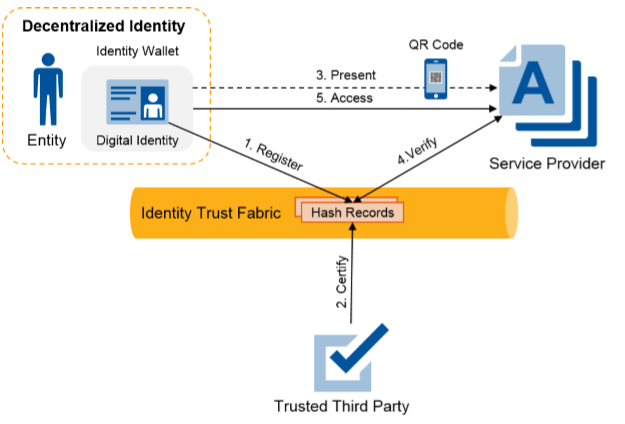
\includegraphics[width=0.9\columnwidth]{diag-comp-flussi.png} 
    \caption{Diagramma flussi tra i vari componenti}
    \label{fig:diag-flussi} 
\end{figure}
Si evidenziano essenzialmente due principali opzioni per la costruzione di questo applicativo. Il primo è l’utilizzo, anche per esso come per l’ITF, di un approccio totalmente distribuito basato su blockchain.  Il secondo approccio consiste i un’applicazione tradizionale.  
\subsubsection{Sviluppo distribuito}  
Questo approccio prevede che la logica applicativa sia totalmente affidata a codice eseguito su blockchain. Questo comporterebbe una disponibilità continuativa sempre garantita e altre caratteristiche di affidabilità e sicurezza. Come punto negativo si evidenzia che una soluzione del genere implicherebbe l’uso di molte tecnologie non completamente mature e di linguaggi in molti casi incompleti. Inoltre questa scelta implicherebbe l’utilizzo della stessa blockchain presente nell’ITF. I vantaggi attribuibili a questo approccio non sono considerati fondamentali al fine di una buona implementazione del SP, di contro gli svantaggi risultano particolarmente pesanti. L’applicazione di un approccio di questo genere anche se possibile risulta sconsigliato. Uno sviluppo di questo tipo, almeno in reti di tipo Permissionless, comporta un cambio di stile di programmazione dovuto all’alto costo delle operazioni. Come descritto nello studio tecnologico Ethereum ciò comporta le seguenti diversità:
\begin{itemize}
    \item alcuni pattern non risultano applicabili;
    \item complessità lineari sono difficilmente giustificabili;
    \item uso di pattern ad hoc.
\end{itemize}
\subsubsection{Sviluppo tradizionale}
La seconda opzione risulta essere una più tradizionale applicazione server che comunica tramite librerie alla blockchain. Si consiglia l’uso di linguaggi fortemente tipati quali: 
\begin{itemize}
    \item C++;
    \item C Sharp;
    \item Java.
\end{itemize}
Data l’alta diffusione di Javascript e NodeJS nella comunità Ethereum si consigliano pure questi.
In base al linguaggio scelto e alla tecnologia blockchain scelta, si dovranno utilizzare differenti librerie per effettuare la comunicazione tra la rete e l’applicativo. Nel caso di Ethereum si propongono le seguenti librerie:
\begin{table}[!h] %
    \caption{Tabella comparivi linguaggio per sviluppo SP}
    \label{tab:comp-ling}
    \begin{tabularx}{\textwidth}{|l|l|l|X|}
    \hline
    \textbf{Linguaggio} & \textbf{Libreria} & \textbf{Note}\\
    \hline
    C++   & cpp-ethereum & - \\
    \hline
    C Sharp   & Nethereum & Questa soluzione si collega particolarmente bene alla scelta di Xamarin per l’IW. \\
    \hline
    JS e NodeJS   & Web3 & -\\
    \hline
    Java  & Web3j & -\\
    \hline
    \end{tabularx}
\end{table}%

Di seguito si procederà alla trattazione di alcuni degli strumenti che si ritengono più utili.
\paragraph{Nethereum}:è un tool che permette una facile integrazione con il client in applicazioni .NET. Fornisce una suite di librerie open source che aiutano a prototipare applicazione .NET velocemente. E’ disponibile anche nel sotto insieme Xamarin.  La documentazione è presente è sembra ben strutturata e di ottima qualità. Inoltre potrebbe rappresentare una buona soluzione in caso di scelta di Microsoft Azure Blockchain. Il sito del progetto è il seguente www.nethereum.com.   
\paragraph{Web3}: è una collezione di librerie che permettono di interagire con un nodo remoto o locale usando una connessione HTTP o IPC. Web3 è presente in npm, meteor, pure js. Per il suo funzionamento è necessario avere un client attivo nel proprio computer. Web3 supporta Mist e Metamask. Il sito del progetto è il seguente: web3js.readthedocs.io.
\paragraph{Web3J}: si tratta di una libreria analoga a Web3 per Java.
\paragraph{Mist}: è un browser sviluppato direttamente dal team Ethereum in grado di operare transazioni direttamente nella blockchain senza la necessità di possedere un intero nodo. È estremamente immaturo e non utilizzabile in produzione. Si riporta di seguito il sito del progetto: github.com/ethereum/mist.
\paragraph{Metamask}: è uno plugin disponibile per i browser Chrome, Firefox e Opera che permette di interfacciarsi alla rete Ethereum senza la necessità di eseguire in intero nodo della rete. Il plugin include un wallet con cui l’utente può inserire il proprio account tramite la chiave privata. Una volta inserito l’account il plugin farà da tramite tra l’applicazione e la rete.
In caso, invece, si opti per la scelta di Hyperledger la scelta risulterebbe molto più semplice in quanto la blockchain in questione fornisce un’API per la comunicazione REST.


\subsubsection{Scelta del client Ethereum}
Il client è un componente che implementa il protocollo di comunicazione di Ethereum. Ethereum diversamente da Hyperledger presenta una realtà molto varia e frattagliata. Solo dal punto di vista del client ci sono multiple implementazioni per differenti sistemi operativi ed in differenti linguaggi. Questa diversità viene vista dalla community come un indicatore di salute per l’intero ecosistema. Il protocollo in ogni caso è sempre lo stesso ed è definito nel così detto Yellow Paper in nota 5, in sostanza si basa sull’utilizzo di file Json. 
Fino al settembre 2016 erano presente le alternative esposte in tabella \ref{tab:comp-client}.
\begin{table}[!h] %
    \caption{Tabella comparivi client Ethereum}
    \label{tab:comp-client}
    \begin{tabularx}{\textwidth}{|X|X|X|}
    \hline
    \textbf{Client} & \textbf{Linguaggio} & \textbf{Sviluppatore}\\
    \hline
    Go-ethereum   & Go & Ethereum Foundation \\
    \hline
    Parity   & Rust & Ethcore \\
    \hline
    Cpp-ethereum   & C++ & Ethereum Foundation\\
    \hline
    Pyethapp  & Python & Ethereum Foundation\\
    \hline
    Ethereumjs-lib  & Javascript & Ethereum Foundation\\
    \hline
    Ethereum(J)  & Java & <ether.camp>\\
    \hline
    Ruby-ethereum  & Ruby & Jan Xie\\
    \hline
    EthereumH  & Haskell & BlockApps\\
    \hline
    \end{tabularx}
\end{table}%
I client appena citati sono accessibili tramite apposite librerie, un buon esempio potrebbe essere web3 per Javascript.
\subsubsection{Scelta del client Hyperledger}
In caso si dovesse optare per una scelta basata su Hyperledger quale base dell’ITF bisognerà ricadere sull’unica soluzione proposta dal team di sviluppo, cioè quella di utilizzare direttamente una comunicazione REST. Il team offre uno strumento detto Composer con il quale si potrà definire un’interfaccia per operare la comunicazione REST. Al fine di poter gestire efficientemente queste chiamate lato applicazione SP si consigliano le librerie esposte in tabella \ref{tab:comp-client-hyp}.
\begin{table}[!h] %
    \caption{Tabella comparivi client Ethereum}
    \label{tab:comp-client-hyp}
    \begin{tabularx}{\textwidth}{|X|X|X|}
    \hline
    \textbf{Linguaggio} & \textbf{Librerie} & \textbf{Sito}\\
    \hline
    .NET   & WCF REST Starter Kit  & \url{www.asp.net/downloads/starter-kits/wcf-rest} \\
    \hline
    .NET   & OpenRasta & \url{www.openrasta.org} \\
    \hline
    .NET   & Service Stack  & \url{www.servicestack.net} \\
    \hline
    Java  & Jersey & \url{www.jersey.java.net} \\
    \hline
    Java  & RESREasy & \url{www.jboss.org/resteasy}\\
    \hline
    Java  & Restlet & \url{www.restlet.org}\\
    \hline
    C++  & linavajo & \url{www.libnavajo.org}\\
    \hline
    C++  & C++ RESTful framework & \url{www.github.com/corvusoft/restbed}\\
    \hline
    C++  & C++ REST SDK & \url{www.github.com/Microsoft/cpprestsdk}\\
    \hline
    \end{tabularx}
\end{table}%
Data l’amplissima diffusione delle API REST e di queste librerie non si procede ad una trattazione analitica.
\subsection{Conclusioni scelta sviluppo}
Considerando quanto precedentemente detto lo sviluppo tradizionale sembrerebbe avrebbe meno incognite e un ampio repertorio di librerie utilizzabili. Si propone, quindi un’architettura del secondo tipo.
Inoltre, si vuole fare notare come l’utilizzo delle soluzioni .NET potrebbero rivelarsi molto vantaggioso in quanto facilmente integrabili con il componente IW e Azure Blockchain.
\subsection{Motivazioni}
\subsubsection{Aspetti positivi}
A seguito dell’analisi sopra proposta sono stati individuati i seguenti aspetti positivi:
\begin{itemize}
    \item lo sviluppo di un’applicazione server tradizionale comporta uno sviluppo molto semplice e immediato, grazie anche alla disponibilità di un ampio repertorio di librerie;
    \item la comunicazione con la blockchain risulta in ogni caso facilmente implementabile grazie all’utilizzo di apposite librerie.
    \item esiste un’ampia scelta di librerie front end per ogni possibile linguaggio di sviluppo.
\end{itemize}
    
\subsubsection{Fattori di rischio}
\begin{risk}{Inesperienza nello sviluppo C Sharp}
    \riskdescription{Non si ha esperienza nello sviluppo di applicazioni C Sharp.}
    \risksolution{Rendere edotto il responsabili del progetto, il quale mettera a disposizione del personale per impartire supporto su C Sharp.}
    \label{risk:centralization-vision-from-user} 
\end{risk}
\begin{risk}{difficoltà di integrazione con Monokee}
    \riskdescription{Il componete SP è il componente che deve essere integrato in Monokee}
    \risksolution{Rendere edotto il responsabili del progetto, il quale mettera a disposizione del personale.}
    \label{risk:centralization-vision-from-user} 
\end{risk}
\begin{risk}{Prestazioni chiamate alla rete blockchain}
    \riskdescription{Il componete SP deve interrogare la rete blockchain, questo potrebbe rappresentare un problema di performance}
    \risksolution{Rendere edotto il responsabili del progetto, valutare soluzioni alternative.}
    \label{risk:centralization-vision-from-user} 
\end{risk}
\subsection{Conclusioni}
Dal presente studio emerge come la creazione di un SP sviluppato come applicativo server, e non come applicazione distribuita, possa essere un’ottima opzione implementativa. Lo studio non presenta particolari rischi. In definitiva, si ritiene che un approccio di questo tipo sia fattibile nei tempi dello stage.
%**************************************************************

\section{Requisiti e obiettivi}

%**************************************************************
\section{Pianificazione}             % Kick-Off
% !TEX encoding = UTF-8
% !TEX TS-program = pdflatex
% !TEX root = ../tesi.tex

%**************************************************************
\chapter{Analisi dei requisiti}
\label{cap:analisi-requisiti}
%**************************************************************

\intro{Breve introduzione al capitolo}\\
Questo capitolo ha lo scopo di fornire una definizione dei requisiti individua per la creazione del prodotto Identity Wallet (IW). Le metodologie usate sono tratte dal capitolo quattro di \cite{som:swe}.
Più in particolare la presente capitolo si prefigge di: 
\begin{itemize}
    \item individuare le fonti per la deduzione dei requisiti; 
    \item dedurre i requisiti dalle fonti; 
    \item descrivere i requisiti individuati; 
    \item catalogare i requisiti individuati; 
    \item prioritizzare i requisiti individuati;
\end{itemize}
\section{Specifiche in Linguaggio Naturale}
Il linguaggio naturale ha un’enorme potenza espressiva ma, essendo inerentemente ambiguo, può portare ad incomprensioni. È quindi necessario limitarne l’utilizzo e standardizzarlo, in modo da ridurre al minimo le possibili ambiguità. È comunque fondamentale evitare di utilizzare espressioni e acronimi che possano essere fraintendibili dagli stakeholders, a tal proposito in fondo al documento è presente una lista degli acronimi utilizzato.
\section{Specifiche in Linguaggio Strutturato}
Il linguaggio strutturato mantiene gran parte dell’espressività del linguaggio naturale, fornendo però uno standard schematico che permette l’uniformità della descrizione dei vari requisiti. Sebbene l’utilizzo di un linguaggio strutturato permetta di organizzare i requisiti in modo più ordinato e comprensibile, talvolta la ridotta espressività rende difficile la definizione di requisiti complessi. A tal proposito è possibile integrare la specifica in linguaggio strutturato con una descrizione in linguaggio naturale.
\section{Specifiche in Linguaggio UML Use Case}
Per la definizione dei diagrammi UML dei casi d’uso, viene utilizzato lo standard UML 2.0 \footcite{site:uml}. Nei diagrammi dei casi d’uso vengono mostrati gli attori coinvolti in un’interazione con il sistema in modo schematico, indicando i nomi delle parti coinvolte. Eventuali informazioni aggiuntive possono essere espresse testualmente.

\section{Analisi dei requisiti IW}
\subsection{Casi d'uso}

Per lo studio dei casi di utilizzo del prodotto sono stati creati dei diagrammi.
I diagrammi dei casi d'uso (in inglese \emph{Use Case Diagram}) sono diagrammi di tipo \gls{uml} dedicati alla descrizione delle funzioni o servizi offerti da un sistema, così come sono percepiti e utilizzati dagli attori che interagiscono col sistema stesso.

\subsubsection{Descrizione Attori}
I tipi di attori principali che andranno ad interagire direttamente con il sistema sono essenzialmente tre: 
\begin{itemize}
    \item utente;
    \item utente non registrato;
    \item utente autenticato. 
\end{itemize}   
Tra di essi è presente una relazione di generalizzazione che vede l’attore utente come generalizzazione degli attori utente non registrato e utente registrato. Questo tipo di generalizzazione viene rappresentata graficamente in figura \ref{fig:ger-actors}.
\begin{figure}[!h]
    
    \centering
    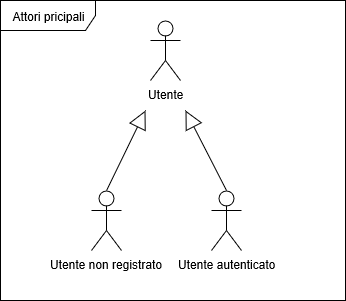
\includegraphics[width=0.5\columnwidth]{usecase/use-case-iw/actors.png} 
    \caption{Gerarchia utenti user case}
    \label{fig:ger-actors} 
\end{figure}
Sono stati individuati i seguenti attori secondari: ITF, MonoKee.
\subsubsection{Attori principali}
\begin{itemize}
    \item \textbf{Utente}: l’attore utente è un fruitore generico del sistema. Potrebbe avere o non avere effettuato l’accesso all’applicazione. Da lui derivano gli attori utente non registrato e utente autenticato.	
    \item \textbf{Utente non registrato}: l’attore utente non registrato è una particolare specializzazione dell’attore utente. Unica sua caratteristica è quella di non essere riconosciuto come utente di MonoKee.
    \item \textbf{Utente autenticato}: l’attore utente autenticato è una particolare specializzazione dell’attore utente. Rappresenta un utente che ha effettuato l’accesso al sistema e che è stato riconosciuto all’interno del sistema MonoKee.
\end{itemize}
      
\subsubsection{Attori secondari}
\begin{itemize}
    \item \textbf{ITF}: è il componente dell’estensione che ha il compito di conservare e convalidare tutte le informazioni provenienti dall’IW.
    \item \textbf{MonoKee}: è il componente centrare dell’attuale servizio MonoKee. Ha il compito di fornire le informazioni di accesso del servizio MonoKee. 
\end{itemize}
    


\subsubsection{UC1: Azioni utente generico}
\begin{figure}[!htbp] 
    \centering 
    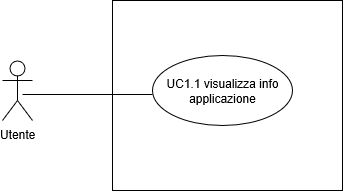
\includegraphics[width=0.7\columnwidth]{usecase/use-case-iw/UC1-azioni-utente.png} 
    \caption{Use Case - UC1: Azioni utente generico}
\end{figure}

\paragraph{Descrizione}  L’utente può visualizzare le informazioni sull’applicazione 
\paragraph{Attore primario}  Utente
\paragraph{Attore secondario}  Nessuno
\paragraph{Precondizioni}  L’utente ha avviato l’applicazione
\paragraph{Postcondizioni}  L’utente ha eseguito le azioni che desiderava compiere in relazione alle sue possibilità
\paragraph{Scenario principale}  
    \begin{enumerate}
        \item UC1.1 Visualizza info applicazione
    \end{enumerate}
\paragraph{Scenari alternativi}  Nessuno


\subsubsection{UC1.1 – Visualizza info applicazione}
\begin{figure}[!htbp] 
    \centering 
    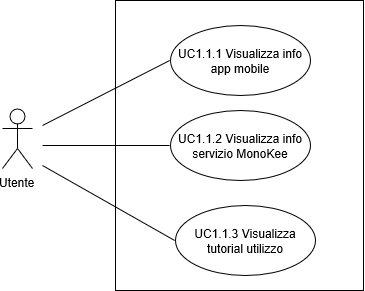
\includegraphics[width=0.7\columnwidth]{usecase/use-case-iw/UC1-1-Visualizza-info-applicazione.png} 
    \caption{Use Case - UC1.1 – Visualizza info applicazione}
\end{figure}

\paragraph{Descrizione}  Il sistema deve visualizzare le informazioni relative all’applicazione mobile e al servizio MonoKee  
\paragraph{Attore primario}  Utente
\paragraph{Attore secondario}  Nessuno
\paragraph{Precondizioni}  L’utente ha avviato l’applicazione
\paragraph{Postcondizioni}  L’utente ha visualizzato le informazioni che desirava riguardo l’applicazione
\paragraph{Scenario principale}  
    \begin{enumerate}
        \item UC1.1.1 Visualizza info applicazione
        \item UC1.1.2 Visualizza info servizio MonoKee
        \item UC1.1.3 Visualizza tutorial utilizzo
    \end{enumerate}
\paragraph{Scenari alternativi}  Nessuno


\subsubsection{UC1.1.1 – Visualizza info app mobile}
\paragraph{Descrizione}  Il sistema deve visualizzare le informazioni tecniche relative all’applicazione mobile
\paragraph{Attore primario}  Utente
\paragraph{Attore secondario}  Nessuno
\paragraph{Precondizioni}  L’utente ha avviato l’applicazione ed ha richiesto la visualizzazione delle informazioni tecniche relative all’applicazione mobile
\paragraph{Postcondizioni}  L’utente ha visualizzato le informazioni con le informazioni tecniche relative all’applicazione mobile
\paragraph{Scenario principale}  
L’utente visualizza un messaggio con le informazioni tecniche relative all’applicazione mobile
\paragraph{Scenari alternativi}  Nessuno


\subsubsection{UC1.1.2 – Visualizza info servizio MonoKee}
\paragraph{Descrizione}  Il sistema deve visualizzare le informazioni relative al servizio MonoKee
\paragraph{Attore primario}  Utente
\paragraph{Attore secondario}  Nessuno
\paragraph{Precondizioni}  L’utente ha avviato l’applicazione ed ha richiesto la visualizzazione delle informazioni relative al servizio MonoKee
\paragraph{Postcondizioni}  L’utente ha visualizzato le informazioni con le informazioni relative al servizio MonoKee
\paragraph{Scenario principale}  
L’utente visualizza un messaggio con le informazioni relative al servizio MonoKee
\paragraph{Scenari alternativi}  Nessuno


\subsubsection{UC1.1.3 – Visualizza tutorial utilizzo}
\paragraph{Descrizione}  Il sistema deve visualizzare un tutorial su come utilizzare l’applicazione IW
\paragraph{Attore primario}  Utente
\paragraph{Attore secondario}  Nessuno
\paragraph{Precondizioni}  L’utente ha avviato l’applicazione ed ha richiesto la visualizzazione di un tutorial su come utilizzare l’applicazione IW
\paragraph{Postcondizioni}  L’utente ha visualizzato il tutorial su come utilizzare l’applicazione IW
\paragraph{Scenario principale}  
L’utente visualizza un tutorial su come utilizzare l’applicazione IW
\paragraph{Scenari alternativi}  Nessuno


\subsubsection{UC2 – Azioni utente non registrato}
\begin{figure}[!htbp] 
    \centering 
    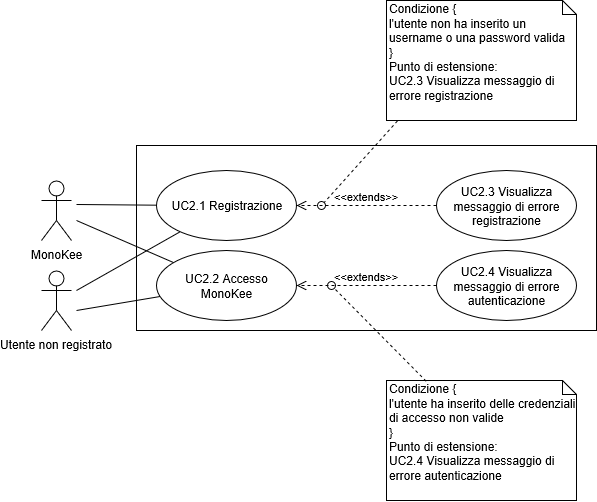
\includegraphics[width=0.7\columnwidth]{usecase/use-case-iw/UC2-azioni-utente-non-registrato.png} 
    \caption{Use Case - UC2: Azioni utente non registrato}
\end{figure}

\paragraph{Descrizione}  L’utente non registrato può eseguire le operazioni di registrazione e accesso al servizio MonoKee 
\paragraph{Attore primario}  Utente non registrato
\paragraph{Attore secondario}  MonoKee
\paragraph{Precondizioni}  L’utente ha avviato l’applicazione ed non è ancora riconosciuto nel sistema
\paragraph{Postcondizioni}  L’utente ha eseguito le azioni che desiderava compiere in relazione alla condizione di non essere registrato
\paragraph{Scenario principale}  
    \begin{enumerate}
        \item UC2.1 Registrazione
        \item UC2.2 Accesso MonoKee
    \end{enumerate}
\paragraph{Scenari alternativi}  
    \begin{enumerate}
        \item l’utente ha fornito dati di registrazione non validi o il doppio inserimento della password non coincide: UC2.3 Visualizzazione messaggio di errore registrazione.
        \item l’utente ha fornito username e password non corrispondenti ha nessun utente registrato al servizio: UC2.4 Visualizzazione messaggio di errore autenticazione.
    \end{enumerate}


\subsubsection{UC2.1 – Registrazione}
\begin{figure}[!htbp] 
    \centering 
    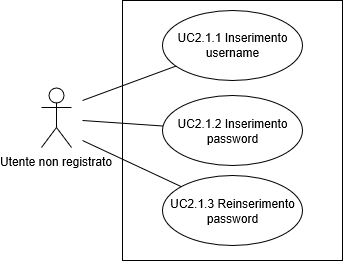
\includegraphics[width=0.7\columnwidth]{usecase/use-case-iw/UC2-1-Registrazione.png} 
    \caption{Use Case - UC2.1: Registrazione}
\end{figure}

\paragraph{Descrizione}  L’utente non registrato può eseguire l’operazione di registrazione 
\paragraph{Attore primario}  Utente non registrato
\paragraph{Attore secondario}  MonoKee
\paragraph{Precondizioni}  L’utente ha avviato l’applicazione, non è ancora riconosciuto nel sistema ed ha espresso la volontà di effettuare la registrazione al servizio MonoKee
\paragraph{Postcondizioni}  L’utente ha eseguito l’operazione di registrazione al sistema
\paragraph{Scenario principale}  
    \begin{enumerate}
        \item UC2.1.1 Inserimento username
        \item UC2.1.2 Inserimento password
        \item UC2.1.3 Reinserimento password
    \end{enumerate}
\paragraph{Scenari alternativi}  Nessuno



\subsubsection{UC2.1.1 – Inserimento username}
\paragraph{Descrizione}  L’utente non registrato deve inserire un username per l’operazione di registrazione
\paragraph{Attore primario}  Utente non registrato
\paragraph{Attore secondario}  Nessuno
\paragraph{Precondizioni}  L’utente ha avviato l’applicazione, non è ancora riconosciuto nel sistema ed il sistema richiede l’inserimento di un username per l’operazione di registrazione
\paragraph{Postcondizioni}  L’utente ha inserito l’username per la registrazione
\paragraph{Scenario principale}  
L’utente non registrato inserisce una stringa tramite l’utilizzo di una text box
\paragraph{Scenari alternativi}  Nessuno


\subsubsection{UC2.1.2 – Inserimento password}
\paragraph{Descrizione}  L’utente non registrato deve inserire una password per l’operazione di registrazione
\paragraph{Attore primario}  Utente non registrato
\paragraph{Attore secondario}  Nessuno
\paragraph{Precondizioni}  L’utente ha avviato l’applicazione, non è ancora riconosciuto nel sistema ed il sistema richiede l’inserimento di una password per l’operazione di registrazione
\paragraph{Postcondizioni}  L’utente ha inserito la password per la registrazione
\paragraph{Scenario principale}  
L’utente non registrato inserisce una stringa tramite l’utilizzo di una text box
\paragraph{Scenari alternativi}  Nessuno



\subsubsection{UC2.1.3 – Reinserimento password}
\paragraph{Descrizione}  L’utente non registrato deve reinserire la password per l’operazione di registrazione
\paragraph{Attore primario}  Utente non registrato
\paragraph{Attore secondario}  Nessuno
\paragraph{Precondizioni}  L’utente ha avviato l’applicazione, non è ancora riconosciuto nel sistema ed il sistema richiede il reinserimento di una password per l’operazione di registrazione
\paragraph{Postcondizioni}  L’utente ha reinserito la password per la registrazione
\paragraph{Scenario principale}  
L’utente non registrato inserisce una stringa tramite l’utilizzo di una text box
\paragraph{Scenari alternativi}  Nessuno



\subsubsection{UC2.2 – Accesso MonoKee}
\begin{figure}[!htbp] 
    \centering 
    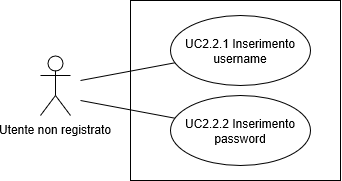
\includegraphics[width=0.7\columnwidth]{usecase/use-case-iw/UC2-2-Accesso-MonoKee.png} 
    \caption{Use Case - UC2.1: Accesso MonoKee}
\end{figure}

\paragraph{Descrizione}  L’utente non registrato può eseguire l’operazione di autenticazione 
\paragraph{Attore primario}  Utente non registrato
\paragraph{Attore secondario}  MonoKee
\paragraph{Precondizioni}  L’utente ha avviato l’applicazione, non è ancora riconosciuto nel sistema ed ha espresso la volontà di effettuare l’autenticazione al servizio MonoKee
\paragraph{Postcondizioni}  L’utente ha eseguito l’operazione di accesso al sistema ed è quindi ora riconosciuto come utente autenticato
\paragraph{Scenario principale}  
    \begin{enumerate}
        \item UC2.1.1 Inserimento username
        \item UC2.1.2 Inserimento password
    \end{enumerate}
\paragraph{Scenari alternativi}  Nessuno


\subsubsection{UC2.2.1 – Inserimento username}
\paragraph{Descrizione}  L’utente non registrato deve inserire un username per l’operazione di autenticazione
\paragraph{Attore primario}  Utente non registrato
\paragraph{Attore secondario}  Nessuno
\paragraph{Precondizioni}  L’utente ha avviato l’applicazione, non è ancora riconosciuto nel sistema ed il sistema richiede l’inserimento di un username per l’operazione di autenticazione
\paragraph{Postcondizioni}  L’utente ha inserito l’username per l’autenticazione
\paragraph{Scenario principale}  
L’utente non registrato inserisce una stringa tramite l’utilizzo di una text box
\paragraph{Scenari alternativi}  Nessuno



\subsubsection{UC2.2.2 – Inserimento password}
\paragraph{Descrizione}  L’utente non registrato deve inserire una password per l’operazione di autenticazione
\paragraph{Attore primario}  Utente non registrato
\paragraph{Attore secondario}  Nessuno
\paragraph{Precondizioni}  L’utente ha avviato l’applicazione, non è ancora riconosciuto nel sistema ed il sistema richiede l’inserimento di una password per l’operazione di autentificazione
\paragraph{Postcondizioni}  L’utente ha inserito la password per l’autentificazione
\paragraph{Scenario principale}  
L’utente non registrato inserisce una stringa tramite l’utilizzo di una text box
\paragraph{Scenari alternativi}  Nessuno



\subsubsection{UC2.3 – Visualizza messaggio di errore registrazione}
\paragraph{Descrizione}  L’utente non registrato fornisce username già esistente o il doppio inserimento della password non coincide
\paragraph{Attore primario}  Utente non registrato
\paragraph{Attore secondario}  Nessuno
\paragraph{Precondizioni}  L’utente ha avviato l’applicazione, non è ancora riconosciuto nel sistema ed il sistema ha inserito un username già esistente o delle password non coincidenti durante la registrazionerichiede l’inserimento di una password per l’operazione di autentificazione
\paragraph{Postcondizioni}  L’utente ha visualizzato un messaggio di errore relativo all’impossibilità di effettuare la registrazione con i dati forniti
\paragraph{Scenario principale}  
L’utente visualizza un messaggio di errore relativo all’impossibilità di effettuare la registrazione con i dati forniti
\paragraph{Scenari alternativi}  Nessuno



\subsubsection{UC2.4 – Visualizza messaggio di errore autenticazione}
\paragraph{Descrizione}  L’utente non registrato fornisce username e password che non corrispondono a nessun utente registrato al servizio MonoKee
\paragraph{Attore primario}  Utente non registrato
\paragraph{Attore secondario}  Nessuno
\paragraph{Precondizioni}  L’utente ha avviato l’applicazione, non è ancora riconosciuto nel sistema ed il sistema ha inserito un username e una password che non corrispondono a nessun utente registrato al servizio MonoKee
\paragraph{Postcondizioni}  L’utente ha visualizzato un messaggio di errore relativo all’impossibilità di effettuare l’autenticazione
\paragraph{Scenario principale}  
L’utente visualizza un messaggio di errore relativo all’impossibilità di effettuare l’autenticazione
\paragraph{Scenari alternativi}  Nessuno



\subsubsection{UC3 – Azioni utente autenticato}
\begin{figure}[!htbp] 
    \centering 
    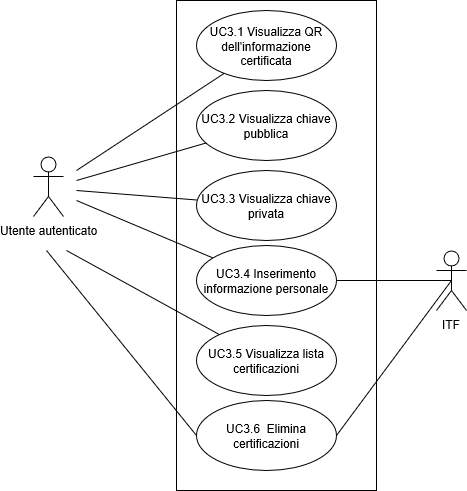
\includegraphics[width=0.7\columnwidth]{usecase/use-case-iw/UC3-Azioni-utente-autententicato.png} 
    \caption{Use Case - UC3: Azioni utente autenticato}
\end{figure}

\paragraph{Descrizione}  L’utente autenticato può eseguire le operazioni legate alla gestione della sua identità e alla presentazione dei propri dati ad un SP
\paragraph{Attore primario}  Utente Autenticato
\paragraph{Attore secondario}  ITF
\paragraph{Precondizioni}  L’utente ha avviato l’applicazione ed è riconosciuto nel sistema come utente di MonoKee
\paragraph{Postcondizioni}  L’utente ha eseguito le azioni che desiderava compiere in relazione alla condizione essere riconosciuto come utente di MonoKee
\paragraph{Scenario principale}  
    \begin{enumerate}
        \item UC3.1 Visualizza QR dell’informazione certificata
        \item UC3.2 Visualizza chiave pubblica
        \item UC3.3 Visualizza chiave privata
        \item UC3.4 Inserimento informazione personale
        \item UC3.5 Visualizza lista certificazioni
        \item UC3.6 Elimina certificazione
    \end{enumerate}
\paragraph{Scenari alternativi}  Nessuno





\subsubsection{UC3.1 – Visualizza QR dell’informazione certificata}
\paragraph{Descrizione}  L’utente autenticato può visualizzare nel proprio schermo un codice QR che rappresenta un’informazione certificata
\paragraph{Attore primario}  Utente Autenticato
\paragraph{Attore secondario}  Nessuno
\paragraph{Precondizioni}  L’utente ha avviato l’applicazione, è riconosciuto nel sistema come utente di MonoKee e ha richiesto di visualizzare il codice QR di una certificazione precedentemente inserita.
\paragraph{Postcondizioni}  L’utente ha visualizzato il codice QR che rappresenta la certificazione selezionata
\paragraph{Scenario principale}  
L’utente seleziona e poi visualizza il codice QR che rappresenta la certificazione selezionata
\paragraph{Scenari alternativi}  Nessuno


\subsubsection{UC3.2 – Visualizza chiave pubblica}
\paragraph{Descrizione}  L’utente autenticato può visualizzare la chiave pubblica generata al momento della registrazione
\paragraph{Attore primario}  Utente Autenticato
\paragraph{Attore secondario}  Nessuno
\paragraph{Precondizioni}  L’utente ha avviato l’applicazione, è riconosciuto nel sistema come utente di MonoKee e ha richiesto la visualizzazione della chiave pubblica.
\paragraph{Postcondizioni}  L’utente ha visualizzato la propria chiave pubblica precedentemente generata
\paragraph{Scenario principale}  
L’utente visualizza la propria chiave pubblica precedentemente generata
\paragraph{Scenari alternativi}  Nessuno



\subsubsection{UC3.2 – Visualizza chiave privata}
\paragraph{Descrizione}  L’utente autenticato può visualizzare la chiave privata generata al momento della registrazione
\paragraph{Attore primario}  Utente Autenticato
\paragraph{Attore secondario}  Nessuno
\paragraph{Precondizioni}  L’utente ha avviato l’applicazione, è riconosciuto nel sistema come utente di MonoKee e ha richiesto la visualizzazione della chiave privata.
\paragraph{Postcondizioni}  L’utente ha visualizzato la propria chiave privata precedentemente generata
\paragraph{Scenario principale}  
L’utente visualizza la propria chiave privata precedentemente generata
\paragraph{Scenari alternativi}  Nessuno



\subsubsection{UC3.4 – Inserimento informazione personale}
\begin{figure}[!htbp] 
    \centering 
    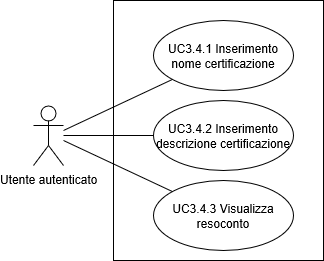
\includegraphics[width=0.7\columnwidth]{usecase/use-case-iw/UC3-4-Inserimento-informazione-personale.png} 
    \caption{Use Case - UC3.4: Inserimento informazione personale}
\end{figure}

\paragraph{Descrizione}  L’utente autenticato può inserire una certificazione e sottometterla all’ITF
\paragraph{Attore primario}  Utente Autenticato
\paragraph{Attore secondario}  ITF
\paragraph{Precondizioni}  L’utente ha avviato l’applicazione, è riconosciuto nel sistema come utente di MonoKee, e ha intende inserire una nuova certificazione alla propria identità
\paragraph{Postcondizioni}  L’utente ha inserito la certificazione e questa è stata presentata all’ITF
\paragraph{Scenario principale}  
    \begin{enumerate}
        \item UC3.4.1 Inserimento nome certificazione
        \item UC3.4.2 Inserimento descrizione certificazione
        \item UC3.4.3 Visualizza resoconto
    \end{enumerate}
\paragraph{Scenari alternativi}  Nessuno



\subsubsection{UC3.4.1 – Inserimento nome certificazione}
\paragraph{Descrizione}  L’utente autenticato deve inserire un nome per l’operazione di inserimento certificazione
\paragraph{Attore primario}  Utente Autenticato
\paragraph{Attore secondario}  Nessuno
\paragraph{Precondizioni}  L’utente ha avviato l’applicazione, è riconosciuto nel sistema ed il sistema richiede l’inserimento di un nome per l’operazione di inserimento certificazione
\paragraph{Postcondizioni}  L’utente ha inserito il nome per l’inserimento della certificazione
\paragraph{Scenario principale}  
L’utente autenticato inserisce una stringa tramite l’utilizzo di una text box
\paragraph{Scenari alternativi}  Nessuno



\subsubsection{UC3.4.2 – Inserimento descrizione certificazione}
\paragraph{Descrizione}  L’utente autenticato deve inserire una descrizione per l’operazione di inserimento certificazione
\paragraph{Attore primario}  Utente Autenticato
\paragraph{Attore secondario}  Nessuno
\paragraph{Precondizioni} L’utente ha avviato l’applicazione, è riconosciuto nel sistema ed il sistema richiede l’inserimento di una descrizione per l’operazione di inserimento certificazione
\paragraph{Postcondizioni}  L’utente ha inserito la descrizione per l’inserimento della certificazione
\paragraph{Scenario principale}  
L’utente autenticato inserisce un insieme di stringhe tramite l’utilizzo di una text box
\paragraph{Scenari alternativi}  Nessuno




\subsubsection{UC3.4.3 – Visualizza resoconto}
\paragraph{Descrizione}  L’utente autenticato può visualizzare un resoconto dei dati inseriti durante la procedura di inserimento certificazione
\paragraph{Attore primario}  Utente Autenticato
\paragraph{Attore secondario}  Nessuno
\paragraph{Precondizioni} L’utente ha avviato l’applicazione, è riconosciuto nel sistema come utente di MonoKee, ha iniziato una procedura di inserimento certificazione e ha richiesto la visualizzazione del resoconto dei dati inseriti
\paragraph{Postcondizioni}  L’utente ha visualizzato un resoconto dei dati inseriti durante la procedura di inserimento certificazione
\paragraph{Scenario principale}  
L’utente visualizza un resoconto dei dati inseriti durante la procedura di inserimento certificazione
\paragraph{Scenari alternativi}  Nessuno






\subsubsection{UC3.5 – Visualizza lista certificazioni}
\begin{figure}[!htbp] 
    \centering 
    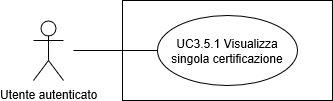
\includegraphics[width=0.7\columnwidth]{usecase/use-case-iw/UC3-5-Visualizza-lista-certificazioni.png} 
    \caption{Use Case - UC3.5: Visualizza lista certificazioni}
\end{figure}

\paragraph{Descrizione}  L’utente autenticato può visualizzare una lista con il nome e l’identificativo della certificazione associate alla propria identità
\paragraph{Attore primario}  Utente Autenticato
\paragraph{Attore secondario}  Nessuno
\paragraph{Precondizioni}  L’utente ha avviato l’applicazione, è riconosciuto nel sistema come utente di MonoKee e ha richiesto la visualizzazione della lista delle certificazioni
\paragraph{Postcondizioni}  L’utente ha visualizzato la lista delle certificazioni
\paragraph{Scenario principale}  
    \begin{enumerate}
        \item UC3.5.1 Visualizza singola certificazione
    \end{enumerate}
\paragraph{Scenari alternativi}  Nessuno





\subsubsection{UC3.5.1 – Visualizza singola certificazione}
\begin{figure}[!htbp] 
    \centering 
    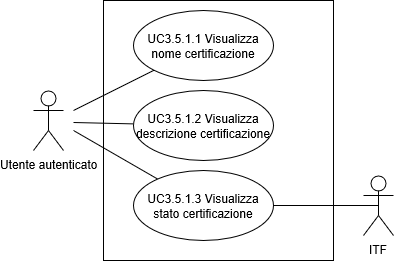
\includegraphics[width=0.7\columnwidth]{usecase/use-case-iw/UC3-5-1-Visualizza-singola-certificazione.png} 
    \caption{Use Case - UC3.5.1: Visualizza singola certificazione}
\end{figure}

\paragraph{Descrizione}  L’utente autenticato può visualizzare i dettagli di una certificazione selezionata della lista delle certificazioni
\paragraph{Attore primario}  Utente Autenticato
\paragraph{Attore secondario}  ITF
\paragraph{Precondizioni}  L’utente ha avviato l’applicazione, è riconosciuto nel sistema come utente di MonoKee e ha richiesto la visualizzazione di una specifica entry della lista delle certificazioni
\paragraph{Postcondizioni}  L’utente ha visualizzato i dettagli di una specifica certificazione della lista
\paragraph{Scenario principale}  
    \begin{enumerate}
        \item UC3.5.1.1 Visualizza nome certificazione
        \item UC3.5.1.2 Visualizza descrizione certificazione
        \item UC3.5.1.3 Visualizza stato certificazione
    \end{enumerate}
\paragraph{Scenari alternativi}  Nessuno




\subsubsection{UC3.5.1.1 – Visualizza nome certificazione}
\paragraph{Descrizione}  L’utente autenticato può visualizzare il nome di una certificazione selezionata della lista delle certificazioni
\paragraph{Attore primario}  Utente Autenticato
\paragraph{Attore secondario}  Nessuno
\paragraph{Precondizioni} L’utente ha avviato l’applicazione, è riconosciuto nel sistema come utente di MonoKee e ha richiesto la visualizzazione del nome di una specifica entry della lista delle certificazioni
\paragraph{Postcondizioni}  L’utente ha visualizzato il nome di una specifica certificazione della lista
\paragraph{Scenario principale}  
L’utente visualizza il nome di una specifica certificazione della lista
\paragraph{Scenari alternativi}  Nessuno




\subsubsection{UC3.5.1.2 – Visualizza descrizione certificazione}
\paragraph{Descrizione}  L’utente autenticato può visualizzare la descrizione di una certificazione selezionata della lista delle certificazioni
\paragraph{Attore primario}  Utente Autenticato
\paragraph{Attore secondario}  Nessuno
\paragraph{Precondizioni} L’utente ha avviato l’applicazione, è riconosciuto nel sistema come utente di MonoKee e ha richiesto la visualizzazione della descrizione di una specifica entry della lista delle certificazioni
\paragraph{Postcondizioni}  L’utente ha visualizzato la descrizione di una specifica certificazione della lista
\paragraph{Scenario principale}  
L’utente visualizza la descrizione di una specifica certificazione della lista
\paragraph{Scenari alternativi}  Nessuno



\subsubsection{UC3.5.1.3 – Visualizza stato certificazione}
\paragraph{Descrizione}  L’utente autenticato può visualizzare lo stato di una certificazione selezionata della lista delle certificazioni. L’informazione proviene dall’ITF.
\paragraph{Attore primario}  Utente Autenticato
\paragraph{Attore secondario}  ITF
\paragraph{Precondizioni} L’utente ha avviato l’applicazione, è riconosciuto nel sistema come utente di MonoKee e ha richiesto la visualizzazione dello stato di una specifica entry della lista delle certificazioni
\paragraph{Postcondizioni}  L’utente ha visualizzato lo stato di una specifica certificazione della lista
\paragraph{Scenario principale}  
L’utente visualizza una stringa che può essere confermata da un TTP o non confermata.
\paragraph{Scenari alternativi}  Nessuno



\subsubsection{UC3.6 – Elimina certificazione}
\paragraph{Descrizione}  L’utente autenticato può eliminare una certificazione selezionata
\paragraph{Attore primario}  Utente Autenticato
\paragraph{Attore secondario}  ITF
\paragraph{Precondizioni} L’utente ha avviato l’applicazione, è riconosciuto nel sistema come utente di MonoKee e ha richiesto l’eliminazione di una specifica certificazione
\paragraph{Postcondizioni}  La certificazione non è più presente dal sistema e pure dall’ITF
\paragraph{Scenario principale}  
L’utente seleziona e poi esprime la volontà di eliminare la certificazione certificata
\paragraph{Scenari alternativi}  Nessuno

















\newpage
\subsection{Tracciamento dei requisiti}

\subsubsection{Fonti}
Per la deduzione dei requisiti utente e di sistema, che verranno presentati nelle sezioni a seguire, sono stati usati come fonti lo studio Gartner \footcite{farah:The-Dawn-of-Decentralized-Identity}, il capitolo \emph{Studio di fattibilità IW} e gli Use Case presentati nella sezione \emph{Casi d'uso}. La struttura e le convenzioni usate sono ispirate dal capitolo di \cite{som:swe}. In seguito vengono riportate le categorie che vengono usate per la catalogazione:
\begin{itemize}
    \item F: requisito funzionale;
    \item V: requisito di vincolo;
    \item Q: requisito di qualità.
\end{itemize}
    
Per l’attribuzione della priorità viene usata la tecnica MoSCoW, quindi gli indici usati sono i seguenti:
\begin{itemize}
    \item M: must;
    \item S: should; 
    \item C: could; 
    \item W: will.
\end{itemize} 
    
Nelle tabelle \ref{tab:requisiti-funzionali}, \ref{tab:requisiti-qualitativi} e \ref{tab:requisiti-vincolo} sono riassunti i requisiti e il loro tracciamento con gli use case delineati in fase di analisi.

\newpage
\begin{center}
\begin{longtable}{|p{2cm}|p{9cm}|p{2cm}|}%
\caption{Tabella del tracciamento dei requisti funzionali}
\label{tab:requisiti-funzionali}
\endfirsthead
\endhead
\hline
\textbf{Codice} & \textbf{Descrizione} & \textbf{Fonte}\\
\hline
R[F][C]0001     & Il sistema potrebbe permettere ad un utente di visualizzare le informazioni dell’applicazione & UC1, UC1.1 \\
\hline
R[F][C]0002     & Il sistema potrebbe permettere di visualizzare le info tecniche dell’applicazione & UC1.1.2 \\
\hline
R[F][C]0003     & Il sistema potrebbe permettere di visualizzare una descrizione del servizio MonoKee & UC1.1.2 \\
\hline
R[F][C]0004     & Il sistema potrebbe permettere di visualizzare un tutorial esplicativo sul suo utilizzo & UC1.1.3 \\
\hline
R[F][M]0005     & Il sistema deve permettere di potersi registrare al servizio & UC2, UC2.1 \\
\hline
R[F][M]0006     & Il sistema deve permettere di essere riconosciuto dal sistema MonoKee & UC2, UC2.2 \\
\hline
R[F][M]0007     & Il sistema deve visualizzare un messaggio di errore in caso i dati forniti durante la registrazione non dovessero essere validi & UC2, UC2.3 \\
\hline
R[F][M]0008     & Il sistema deve visualizzare un messaggio di errore in caso i dati forniti durante la procedura di autenticazione non dovessero essere corretti & UC2, UC2.4 \\
\hline
R[F][M]0009     & Il sistema deve permettere di inserire uno username nell’ottica della procedura di registrazione  & UC2.1.1\\
\hline
R[F][M]0010    & Il sistema deve permettere di inserire una password nell’ottica della procedura di registrazione & UC2.1.2 \\
\hline
R[F][M]0011     & Il sistema deve permettere di reinserire la password nell’ottica della procedura di registrazione & UC2.1.3 \\
\hline
R[F][M]0012     & Il sistema deve permettere di inserire uno username nell’ottica della procedura di autentificazione & UC2.2.1 \\
\hline
R[F][M] 0013     & Il sistema deve permettere di inserire una password nell’ottica della procedura di autentificazione & UC2.2.2 \\
\hline
R[F][M] 0014     & Il sistema deve permettere ad un utente autenticato di poter generare un codice QR di un certificato inserito nel sistema & UC3, UC3.1 \\
\hline
R[F][M] 0015     & Il sistema deve permettere ad un utente autenticato di visualizzare la chiave pubblica & UC3, UC3.2 \\
\hline
R[F][M] 0016     & Il sistema deve permettere ad un utente autenticato di visualizzare la chiave privata & UC3, UC3.3 \\
\hline
R[F][M] 0017     & Il sistema deve permettere ad un utente autenticato di inserire un’informazione personale & UC3, UC3.4 \\
\hline
R[F][M] 0018     & Il sistema deve permettere ad un utente autenticato di visualizzare una lista di certificazioni associate alla propria identità & UC3, UC3.5 \\
\hline
R[F][M] 0019     & Il sistema deve permettere ad un utente autenticato di eliminare una certificazione associata alla propria identità & UC3, UC3.6 \\
\hline
R[F][M] 0020     & Il sistema deve permettere ad un utente autenticato di inserire il nome della certificazione nel contesto dell’inserimento di certificazione & UC3.4.1 \\
\hline
R[F][M] 0021     & Il sistema deve permettere ad un utente autenticato di una descrizione della certificazione nel contesto dell’inserimento di una certificazione & UC3.4.2 \\
\hline
R[F][M] 0022     & Il sistema deve permettere ad un utente autenticato di visualizzare un resoconto dei dati inseriti durante la procedura di inserimento certificato & UC3.4.3 \\
\hline
R[F][M] 0023     & Il sistema deve permettere ad un utente autenticato di visualizzare i dettagli di una singola certificazione & UC3.5.1 \\
\hline
R[F][M] 0024     & Il sistema deve permettere ad un utente autenticato di visualizzare il nome di una certificazione esistente & UC3.5.1.1 \\
\hline
R[F][M] 0025     & Il sistema deve permettere ad un utente autenticato di visualizzare la certificazione di una certificazione esistente & UC3.5.1.2 \\
\hline
R[F][S] 0026     & Il sistema dovrebbe permettere ad un utente autenticato di visualizzare lo stato di una certificazione esistente & UC3.5.1.3 \\
\hline
\end{longtable}%
\end{center}


\begin{center}
\begin{longtable}{|p{2cm}|p{9cm}|p{2cm}|}%
\caption{Tabella del tracciamento dei requisiti di vincolo}
\label{tab:requisiti-vincolo}
\endfirsthead
\endhead
\hline
\textbf{Codice} & \textbf{Descrizione} & \textbf{Fonte}\\
\hline
R[V][M] 0027    & Il sistema deve offrire le proprie funzionalità come applicazione mobile &  IW Studio di fattibilità \\
\hline
R[V][M] 0028    & Il sistema è implementato tramite l’uso di Xamarin & IW Studio di fattibilità \\
\hline
R[V][M] 0029    & Il progetto prevede almeno i seguenti quattro ambienti di sviluppo: Local, Test, Staging, Production & IW Studio di fattibilità \\
\hline
R[V][M] 0030    & Il prodotto è sviluppato utilizzando uno strumento di linting & IW Studio di fattibilità \\
\hline
R[V][M] 0031    & Il sistema deve mantenere la chiave privata sempre in locale & IW Studio di fattibilità \\
\hline
\end{longtable}
\end{center}%



\begin{center}
    \begin{longtable}{|p{2cm}|p{9cm}|p{2cm}|}%
    \caption{Tabella del tracciamento dei requisiti qualitativi}
    \label{tab:requisiti-qualitativi}
    \endfirsthead
    \endhead
    \hline
    \textbf{Codice} & \textbf{Descrizione} & \textbf{Fonte}\\
    \hline
    R[Q][S] 0032    & Il progetto prevede un ragionevole set di test di unità e di test di integrazione & - \\
    \hline
    R[Q][S] 0033   & I test possono essere eseguiti localmente o come parte di integrazione continua & - \\
    \hline
    R[Q][S] 0034    & Il sistema solo alla fine sarà testato nel network pubblico di prova & - \\
    \hline
    R[Q][S] 0035    & Il codice sorgente del prodotto e la documentazione necessaria per l’utilizzo sono versionati in repository pubblici usando GitHub, BitBucket o GitLab & - \\
    \hline
    R[Q][C] 0036    & Lo sviluppo si eseguirà utilizzano un approccio incrementale  & IW Studio di fattibilità \\
    \hline
    \end{longtable}
    \end{center}%

\begin{center}
    \begin{longtable}{|p{3cm}|p{3cm}|}%
    \caption{Tabella del tracciamento dei requisiti con le fonti}
    \label{tab:requisiti-fonte}
    \endfirsthead
    \endhead
    \hline
    \textbf{Codice}  & \textbf{Fonte}\\
    \hline
    R[F][C]0001    & UC1, UC1.1  \\
    \hline
    R[F][C]0002   & UC1.1.2  \\
    \hline
    R[F][C]0003    & UC1.1.2  \\
    \hline
    R[F][C]0004    & UC1.1.3  \\
    \hline
    R[F][M]0005    & UC2, UC2.1  \\
    \hline
    R[F][M]0006    & UC2, UC2.2  \\
    \hline
    R[F][M]0007    & UC2, UC2.3  \\
    \hline
    R[F][M]0008    & UC2, UC2.4  \\
    \hline
    R[F][M]0009    & UC2.1.1  \\
    \hline
    R[F][M]0010    & UC2.1.2  \\
    \hline
    R[F][M]0011    & UC2.1.3  \\
    \hline
    R[F][M]0012    & UC2.2.1  \\
    \hline
    R[F][M] 0013    & UC2.2.2  \\
    \hline
    R[F][M] 0014    & UC3, UC3.1  \\
    \hline
    R[F][M] 0015    & UC3, UC3.2  \\
    \hline
    R[F][M] 0016    & UC3, UC3.3  \\
    \hline
    R[F][M] 0017    & UC3, UC3.4  \\
    \hline
    R[F][M] 0018    & UC3, UC3.5  \\
    \hline
    R[F][M] 0019    & UC3, UC3.6  \\
    \hline
    R[F][M] 0020    & UC3.4.1  \\
    \hline
    R[F][M] 0021    & UC3.4.2  \\
    \hline
    R[F][M] 0022    & UC3.4.3  \\
    \hline
    R[F][M] 0023    & UC3.5.1  \\
    \hline
    R[F][M] 0024    & UC3.5.1.1  \\
    \hline
    R[F][M] 0025    & UC3.5.1.2  \\
    \hline
    R[F][S] 0026    & UC3.5.1.3  \\
    \hline
    R[V][M] 0027    & IW Studio di fattibilità  \\
    \hline
    R[V][M] 0028    & IW Studio di fattibilità  \\
    \hline
    R[V][M] 0029    & IW Studio di fattibilità  \\
    \hline
    R[V][M] 0030    & IW Studio di fattibilità  \\
    \hline
    R[V][M] 0031    & IW Studio di fattibilità  \\
    \hline
    R[Q][S] 0032    & -  \\
    \hline
    R[Q][S] 0033    & -  \\
    \hline
    R[Q][S] 0034    & -  \\
    \hline
    R[Q][S] 0035    & -  \\
    \hline
    R[Q][C] 0036    & IW Studio di fattibilità  \\
    \hline
    \end{longtable}
    \end{center}%

\begin{center}
    \begin{longtable}{|p{3cm}|p{3cm}|}%
    \caption{Tabella del tracciamento delle fonti con i requisiti}
    \label{tab:fonte-req}
    \endfirsthead
    \endhead
    \hline
    \textbf{Fonte}  & \textbf{Codice}\\
    \hline
    UC1    & R[F][C]0001  \\
    \hline
    UC1.1   & R[F][C]0001  \\
    \hline
    UC1.1.2    & R[F][C]0002  \\
    \hline
    UC1.1.2    & R[F][C]0003  \\
    \hline
    UC2   & R[F][M]0005, R[F][M]0006, R[F][M]0007, R[F][M]0008 \\
    \hline
    UC2.1    & R[F][M]0005  \\
    \hline
    UC2.2    & R[F][M]0006  \\
    \hline
    UC2.3    & R[F][M]0007  \\
    \hline
    UC2.4 & R[F][M]0008 \\
    \hline
    UC2.1.1 & R[F][M]0009 \\
    \hline
    UC2.1.2 & R[F][M]0010 \\
    \hline
    UC2.1.3 & R[F][M]0011 \\
    \hline
    UC2.2.1 & R[F][M]0012 \\
    \hline
    UC2.2.2 & R[F][M] 0013 \\
    \hline
    UC3 & R[F][M] 0014, R[F][M] 0015, R[F][M] 0016, R[F][M] 0017, R[F][M] 0018, R[F][M] 0019\\
    \hline
    UC3.1 & R[F][M] 0014 \\
    \hline
    UC3.2 & R[F][M] 0015 \\
    \hline
    UC3.3 & R[F][M] 0016 \\
    \hline
    UC3.4 & R[F][M] 0017 \\
    \hline
    UC3.5 & R[F][M] 0018 \\
    \hline
    UC3.6 & R[F][M] 0019 \\
    \hline
    UC3.4.1 & R[F][M] 0020 \\
    \hline
    UC3.4.2 & R[F][M] 0021 \\
    \hline
    UC3.4.3 & R[F][M] 0022 \\
    \hline
    UC3.5.1 & R[F][M] 0023 \\
    \hline
    UC3.5.1.1 & R[F][M] 0024 \\
    \hline
    UC3.5.1.2 & R[F][M] 0025 \\
    \hline
    UC3.5.1.3 & R[F][S] 0026 \\
    \hline
    IW Studio di fattibilità & R[V][M] 0027, R[V][M] 0028, R[V][M] 0029, R[V][M] 0030, R[V][M] 0031, R[Q][C] 0036 \\
    \hline
    - & R[Q][S] 0032, R[Q][S] 0033, R[Q][S] 0034, R[Q][S] 0035 \\
    \hline
    \end{longtable}
    \end{center}%

\section{Analisi dei requisiti SP}
\subsection{Casi d'uso}

Per lo studio dei casi di utilizzo del prodotto sono stati creati dei diagrammi.
I diagrammi dei casi d'uso (in inglese \emph{Use Case Diagram}) sono diagrammi di tipo \gls{uml} dedicati alla descrizione delle funzioni o servizi offerti da un sistema, così come sono percepiti e utilizzati dagli attori che interagiscono col sistema stesso.

\subsubsection{Descrizione Attori}
I tipi di utente che andranno ad interagire direttamente con il sistema si dividono in due categorie: 
\begin{itemize}
    \item Servizio convenzionato;
    \item Utente IW.
\end{itemize}
Tra gli attori precedentemente citati non è però prevista alcuna funzionalità in comune e non emerge quindi la necessità di avere una gerarchia. In immagine \ref{fig:ger-actors-sp} è proposta una visualizzazione grafica di quanto detto.
Non sono stati individuati, invece, attori secondari che partecipano al sistema.
\begin{figure}[!h]    
    \centering
    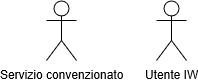
\includegraphics[width=0.5\columnwidth]{usecase/use-case-sp/attori.png} 
    \caption{Gerarchia utenti user case}
    \label{fig:ger-actors-sp} 
\end{figure}
             % Concept Preview
% !TEX encoding = UTF-8
% !TEX TS-program = pdflatex
% !TEX root = ../tesi.tex

%**************************************************************
\chapter{Progettazione e codifica}
\label{cap:progettazione-codifica}
%**************************************************************

\intro{Breve introduzione al capitolo}\\
Il presente capitolo ha lo scopo di presentare e dimostrare l'architettura per i componenti IW e SP che dovranno funzionare nel contesto dell'estensione del prodotto Monokee.
%**************************************************************
\section{Componente Identity Wallet}
Questa sezione inizia con una generica introduzione all’architettura \emph{Xamarin} ed si conclude conclude presentando una prima ipotesi di architettura in formato UML 2.0.
\subsection{Tecnologie e strumenti}
\label{sec:tecnologie-strumenti}
Il componente \emph{Identity Wallet} è sviluppato come applicazione mobile. Questo contesto implica differenti tecnologie che comunicano e interagiscono fra loro. Le funzionalità di persistenza vengono offerte tramite tre diverse tecnologie: \emph{file system}, \emph{blockchain}, e server \emph{Monokee}. La logica di \emph{business} è implementata usando il \emph{framework} .NET. L’interfaccia, invece, usa il pattern MVVM (\emph{Model View View Model}).
L’IW utilizza una classica architettura a strati (\emph{N-tier architecture}). Trattandosi di un sistema mobile multi piattaforma questa architettura è stata calata nel contesto e quindi si è deciso di basarla sul concetto di \emph{Portable Class Libraries} (PCL) presentato da \emph{Xamarin}. 

\subsubsection{Portable Class Libraries PCL}
\gls{pclg}\glsfirstoccur è un approccio alla condivisione del codice tra le diverse edizioni dell’app destinate a diversi sistemi operativi mobili sviluppati da \emph{Xamarin}. Segue un diagramma esplicativo di come si sviluppa una tipica architettura PCL. Il diagramma in figura \ref{fig:ark-pcl} è tratto da \url{www.xamarin.com}.

\begin{figure}[!h]
    
    \centering
    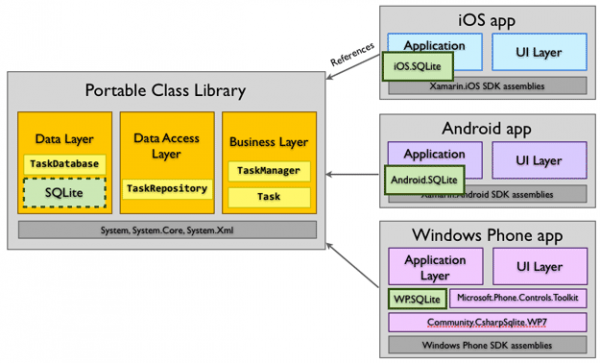
\includegraphics[width=0.9\columnwidth]{ark-pcl.png} 
    \caption{Architettura PCL}
    \label{fig:ark-pcl} 
\end{figure}

Ogni \emph{“Platform-Specific Application Project”} (\emph{iOS app}, \emph{Android app}, \emph{Windows Phone app}) referenzia la \gls{pclg}. Esistono essenzialmente due parti: quelle specifiche per la piattaforma e quelle condivise. Obiettivo del progetto è quello di rendere meno corpose possibile le parti specifiche. Sarà poi possibile impiegare caratteristiche di una determinata piattaforma attraverso l’utilizzo del design pattern \emph{Dependency Injection} (DI).
Applicare i principi della DI significa definire nel codice condiviso interfacce (classi astratte) che vengono implementate (estese) in ogni piattaforma tramite sottoclassi (\emph{Strategy Pattern}). A questo punto sarà possibile integrare le specifiche implementazioni all’interno della PCL. \emph{Xamarin} per questo scopo offre la classe \emph{DependencyService}.

\subsection{Overview}
Come già detto, l’applicativo è strutturato come una \emph{N-tier application} consistente dei seguenti \emph{layer}:
\begin{itemize}
    \item layer presentazione;
    \item logica di business;
    \item layer di accesso ai dati. 
\end{itemize}
    
Quando si sviluppa un’applicazione è importante scegliere se sviluppare un \emph{thin Web-based client} o \emph{un rich client}. Ovviamente, considerando il nostro contesto, ricadiamo nel primo caso, infatti quasi tutta la logica e la persistenza rientrano sul componente ITF. In figura \ref{fig:ark-iw} un'immagine esplicativa dell'architettura ideata.
\begin{figure}[htbp]
    
    \centering
    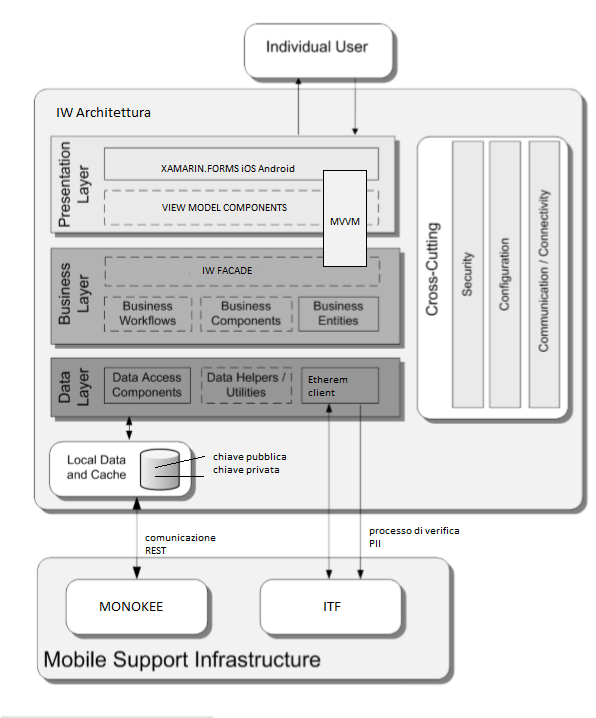
\includegraphics[width=0.9\columnwidth]{ark-iw.png} 
    \caption{Architettura PCWL}
    \label{fig:ark-iw} 
\end{figure}
Come si può notare il principale pattern utilizzato per gestire l’interazione con l’utente è il \emph{Model View ViewModel} (MVVM). Tutte le elaborazioni vengono effettuate dallo strato di \emph{business}, mentre per la persistenza ci si affida principalmente alla risorsa \emph{Monokee} tramite comunicazione REST, oppure all’ITF tramite l’utilizzo di un client \emph{Ethereum}. Tutto verrà sviluppato utilizzando il \emph{framework} .NET.

%**************************************************************
\subsection{Progettazione}
\label{sec:progettazione}
In figura \ref{fig:ark-mod-iw} viene presentato il diagramma di massima dell’architettura dell’IW. Il diagramma è stata redatto seguendo lo standard \emph{UML 2.0}. Subito a seguire viene descritta ogni classe.
\begin{figure}[htbp]
    
    \centering
    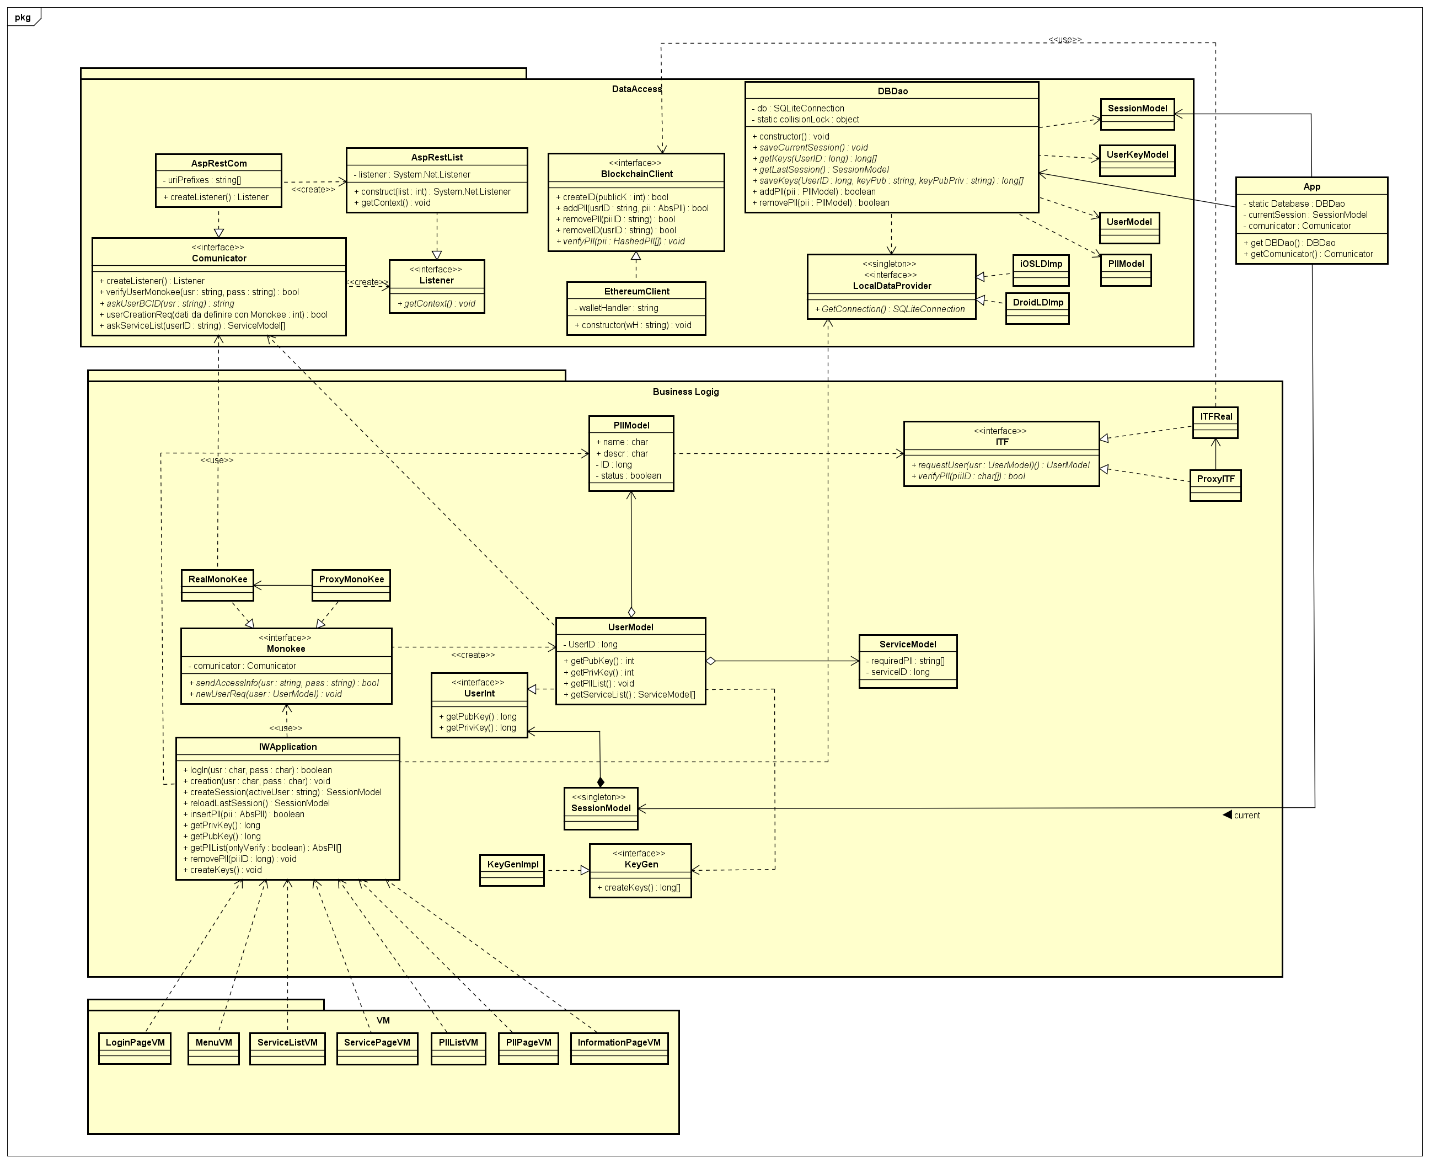
\includegraphics[width=0.9\columnwidth]{iw-complete-uml.png} 
    \caption{Architettura IW}
    \label{fig:ark-mod-iw} 
\end{figure}

\subsubsection{BusinessLogic} %**************************
Nel contesto dell’architettura \emph{N-tier} adottata, il \emph{BusinessLogic layer} è un gruppo di classi che si occupa di effettuare e di mantenere tutte le regole definite dai documenti IW - Analisi di massima, IW – Studio di fattibilità.  

\begin{figure}[htbp]
    \centering
    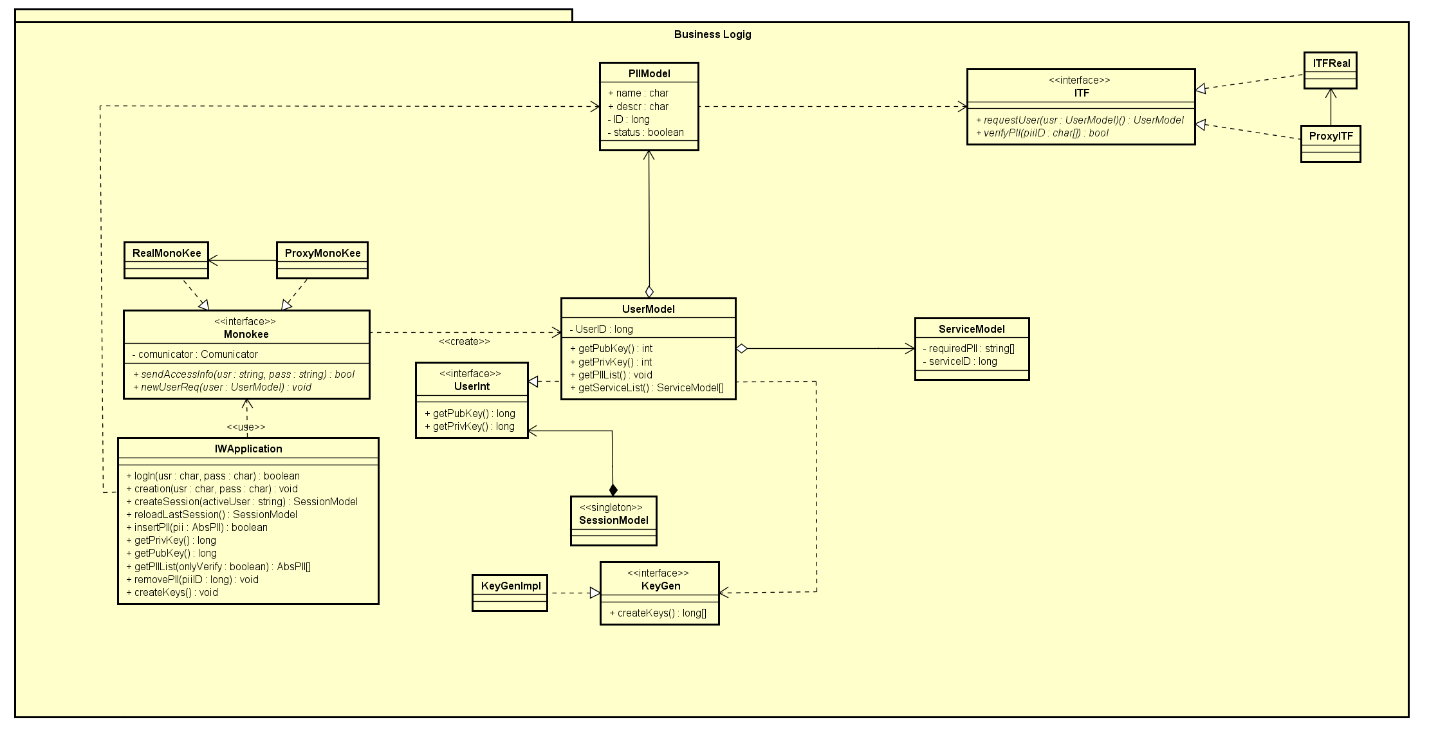
\includegraphics[width=0.9\columnwidth]{bl-lay-iw.png} 
    \caption{Diagramma BusinessLogic Layer IW}
    \label{fig:bl-lay-iw} 
\end{figure}
\begin{namespacedesc}
    \classdesc{IWApplication}{classe che ha il compito di fornire una \emph{facade} per i vari \emph{ViewModel}, di conseguenza tutte le azioni possibili tramite l’interfaccia sono implementate da essa.}

    \classdesc{Monokee}{interfaccia che ha il compito di fornire un’astrazione del servizio \emph{Monokee}. L' interfaccia con \emph{RealMonokee} e \emph{ProxyMonokee} rappresenta un’applicazione del pattern \emph{Proxy}.}

    \classdesc{RealMonokee}{classe che rappresenta il reale oggetto \emph{Monokee} e che dialoga poi con \emph{RESTComp} per ottenere i dati. Questa classe con \emph{RealMonokee} e \emph{ProxyMonokee} rappresenta un’applicazione del pattern \emph{Proxy}.}

    \classdesc{ProxyMonokee}{classe che rappresenta un \emph{proxy} dell’oggetto \emph{Monokee}, questa classe applica una politica di acquisizione pigra. Questa classe con \emph{RealMonokee} e \emph{ProxyMonokee} rappresenta un’applicazione del pattern \emph{Proxy}.}

    \classdesc{KeyGen}{interfaccia che ha lo scopo di definire una strategia di generazione chiavi. Fa parte di un’applicazione dello \emph{Strategy Pattern} ed è stata pensata in un’ottica in cui vi possano essere vari modi per generare una chiave a seconda del sistema operativo usato.}

    \classdesc{KeyGenImpl}{classe che rappresenta una possibile implementazione dell’interfaccia \emph{KeyGen}. Fa parte di un’applicazione dello \emph{Strategy pattern}.}

    \classdesc{Session}{classe con lo scopo di immagazzinare tutti i dati di una sessione attiva; questa può essere generata dal \emph{file system} o creata da zero. Deve essere presente in istanza singola e inoltre contiene le informazioni utente.}

    \classdesc{UserInt}{interfaccia che rappresenta un qualsiasi utente dell’applicazione. È implementata solamente da \emph{UserMonokee}. Questo oggetto viene creato dall’interfaccia \emph{Monokee}.}

    \classdesc{UserMonokee}{classe che rappresenta un utente proveniente dal server \emph{Monokee}. Implementa l’interfaccia \emph{UserInt}. Un utente di questo tipo possiede un aggregato di servizi e una lista PII; potenzialmente può contenere le chiavi.}

    \classdesc{Service}{classe che rappresenta un servizio di cui l’utente ha diritto. Possiede un ID e fornisce una lista di PII che dovranno essere presentati al fine di eseguire l’accesso.}

    \classdesc{KeyProv}{classe che ha il compito di occuparsi della generazione delle chiavi private e pubbliche. Viene usata da \emph{UserInt} e a sua volta usa \emph{LocalDataProvider}.}

    \classdesc{LocalDataProvider}{interfaccia che ha il compito di fornire in singolo punto dove ottenere informazione dal \emph{file system} locale. Successivamente deve essere implementata in base al sistema operativo su cui girerà. }

    \classdesc{iOSLDImp}{rappresenta l’implementazione per \emph{iOS} di \emph{LocalDataProvider}.}

    \classdesc{DroidLDImp}{rappresenta l’implementazione \emph{Android} di \emph{LocalDataProvider}.}

    \classdesc{AbsPII}{interfaccia che rappresenta una generica PII. Ha una sola possibile implementazione, ma può rendere più semplice l’implementazione di future PII.}

    \classdesc{PIIImpl}{classe che rappresenta l’attuale ed unica PII. Consiste di un nome, un identificativo e una descrizione. Una PII può essere verificata o meno tramite l’uso di \emph{PIIChecker}. }

    \classdesc{ITF}{interfaccia che ha il compito di fornire un’astrazione del componente \emph{Identity Trust Fabric}. Con \emph{ITFReal} e \emph{ProxyITF} rappresenta un’applicazione del pattern \emph{Proxy}.}
    \classdesc{RealITF}{classe che rappresenta il reale oggetto ITF. Essa dialoga poi con il \emph{BlockchainClient} per ottenere i dati. Con \emph{RealITF} e \emph{ProxyITF} rappresenta un’applicazione del pattern \emph{Proxy}.}
    \classdesc{ProxyITF}{classe che rappresenta un \emph{proxy} dell’oggetto \emph{Monokee}. Applica una politica di acquisizione pigra. Con \emph{RealITF} e \emph{ProxyITF} rappresenta un’applicazione del pattern \emph{Proxy}.}
    \classdesc{PIIChecher}{classe che ha il compito di verificare tramite ITF la veridicità di una PII.}
\end{namespacedesc}

\subsubsection{DataAccess Layer} %**************************
Nel contesto dell’architettura \emph{N-tier} adottata il \emph{DataAccess layer} è un gruppo di classi che si occupano di interfacciarsi con gli strumenti di persistenza utilizzati dall’applicazione. Questi sono: \emph{Monokee} (tramite RESTful), ITF e una base di dati locale al dispositivo. 
\begin{figure}[htbp]
    \centering
    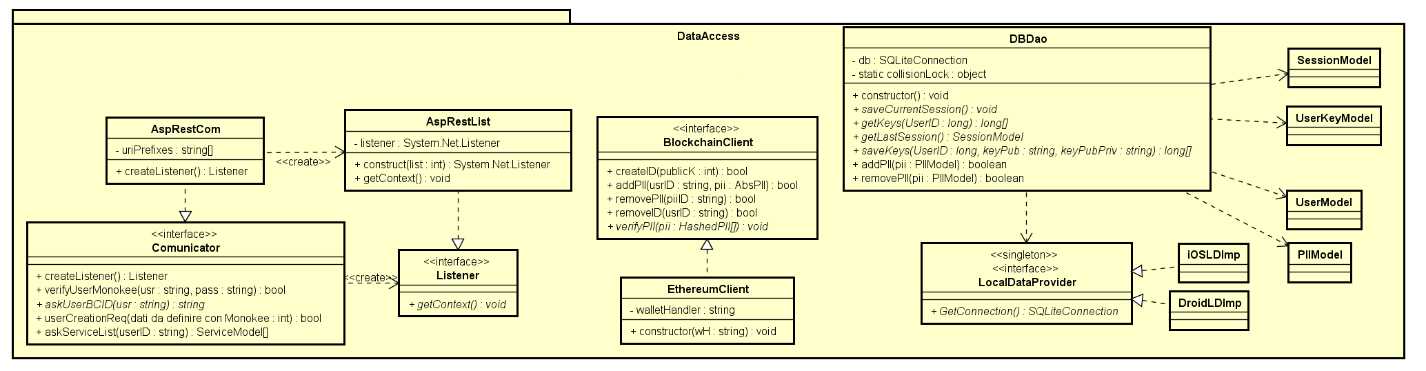
\includegraphics[width=0.9\columnwidth]{dla-iw.png} 
    \caption{Diagramma DataAccess Layer IW}
    \label{fig:dla-iw} 
\end{figure}

\begin{namespacedesc}
    \classdesc{RestComp}{interfaccia che ha il compito di rappresentare una generica strategia di comunicazione REST. Essa viene utilizzata da \emph{RealMonokee} per ottenere i dati relativi all’utente.}
    \classdesc{RestImpl}{possibile implementazione della strategia di comunicazione REST. Implementa l’interfaccia \emph{RestComp}.}
    \classdesc{BlockchainClient}{interfaccia che ha il compito di rappresentare una generica strategia di comunicazione con la rete \emph{blockchain}. Questa astrazione permette di slegare dall’architettura dipendenze con le varie implementazioni di \emph{blockchain} e anche di \emph{client}.}
    \classdesc{EthereumClient}{possibile implementazione di \emph{BlockchainClient} che utilizza la rete \emph{Ethereum}. Questa classe poi userà la libreria \emph{Nethereum}.}
\end{namespacedesc}



\subsubsection{PresentationLayer} %**************************
Questo \emph{layer} contiene i vari controllori che gestiscono le viste. Si è previsto di creare un controller per ogni pagina dell’applicazione. L’applicazione utilizza il pattern MVVM, quindi, i controlliri sono delle \emph{ViewModel} (VM) che contengono i dati e le operazioni. Tra i dati e la vista sono presenti dei \emph{binding} da realizzare utilizzando gli strumenti forniti da \emph{Xamarin}. Le VM operano le loro azioni tramite l’utilizzo della classe \emph{IWFacade}. 


Tutte queste classi devono estendere da \emph{INotifyPropertyChanged}.
In figura \ref{fig:vm-layer-iw} il diagramma esplicativo del \emph{layer}.

\begin{figure}[htbp]
    \centering
    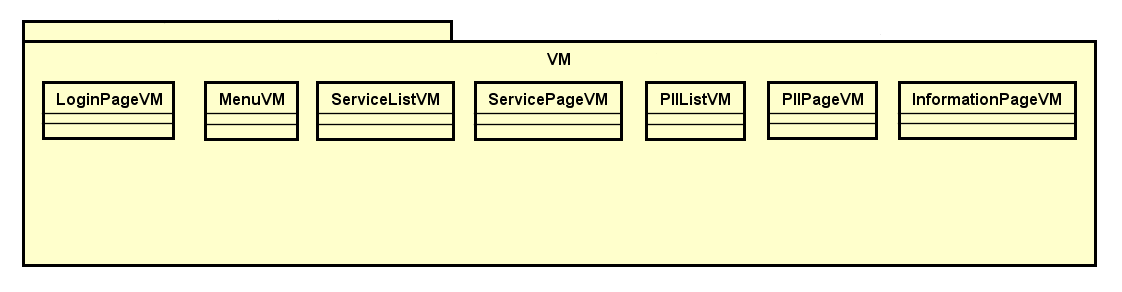
\includegraphics[width=0.9\columnwidth]{VMlayer-iw.png} 
    \caption{Diagramma UML VM Layer}
    \label{fig:vm-layer-iw} 
\end{figure}

\begin{namespacedesc}
    \classdesc{LoginPageVM}{classe che ha lo scopo di gestire la pagina di \emph{log in} e quindi avere lo stato e le operazioni necessarie.}
    \classdesc{MenuVM}{classe che ha lo scopo di gestire il menù dell’applicazione e quindi avere lo stato e le operazioni necessarie.}
    \classdesc{ServiceListVM}{classe che ha lo scopo di gestire la pagina che presenta la lista dei service a cui può accedere l’utente e quindi avere lo stato e le operazioni necessarie.}
    \classdesc{ServicePage}{classe che ha lo scopo di gestire la pagina con le informazioni relative ad un singolo servizio e quindi avere lo stato e le operazioni necessarie.}
    \classdesc{PIIListVM}{classe che ha lo scopo di gestire la pagina che presenta la lista delle PII che possiede l’utente e quindi avere lo stato e le operazioni necessarie.}
    \classdesc{PIIPageVM}{classe con lo scopo di gestire la pagina che visualizza le informazioni relative ad una specifica PII e quindi avere lo stato e le operazioni necessarie.}
    \classdesc{InformationPageVM}{classe che ha lo scopo di gestire la pagina che fornisce le informazioni sull’applicazione, sul servizio \emph{Monokee} e le istruzioni per l’uso.}
\end{namespacedesc}
%**************************************************************
\subsection{Design Pattern utilizzati}
Al fine di garantire elevate doti di qualità e manutenibilità dell’architettura sono stati usati una serie di design pattern. Di seguito segue una breve descrizione di questi.

\paragraph{Communicator}: incapsula i dettagli interni della comunicazione in un componente separato che poi può essere implementato usando tecnologie diverse; risultato utile per rendere gli altri componenti quanto più indipendenti da come comunicano con l’esterno.

\paragraph{Data Transfer Object (DTO)}: oggetto che ha il compito di racchiudere le informazioni utili a diverse componenti. Va a ridurre i metodi necessari per la comunicazione e, in generale, la semplifica.

\paragraph{Entity Translator}: oggetto che trasforma un dato in forma utile per essere usato nella logica di \emph{business}. Esso è stato usato per interfacciarsi con il \emph{client Ethereum} e il \emph{server Monokee}.

\paragraph{Lazy Acquisition Proxy}: Ritarda l’acquisizione delle risorse il più a lungo possibile. Esso è stato ampiamente utilizzato, specialmente per rendere più leggera possibile la creazione dei dati dell’utente e della verifica dei dati nell’ITF.

\paragraph{Strategy Pattern}: oggetto che permette di separare l’esecuzione di un metodo dalla classe che lo contiene. Usando un’interfaccia per astrarre il metodo è poi possibile creare molteplici implementazioni. Ciò è risultato molto utile nel contesto di un’applicazione multi piattaforma in cui alcune procedure dovevano essere implementate in nativo. Oltretutto ha reso possibile separare il metodo dall’implementazione.

\paragraph{Dependency Injection}: pattern che permette di delegare il controllo della creazione oggetti ad un oggetto esterno. Esso permette di semplificare la gestione delle dipendenze e, nel contesto dello \emph{strategy pattern}, permette di inserire l’implementazione corretta.

\paragraph{Model-View-Controller}: separa il codice per l’interfaccia grafica in tre componenti separati: Modello (il dato), Vista (l’interfaccia), e Controllore (il responsabile della logica), con particolare attenzione alla vista. Nel progetto viene usata una sua particolare declinazione chiamata MVVM. 

%**************************************************************


%COMPONENTE SP ********************************************************************
\newpage
\section{Componente Service Provider}
La sezione inizia con una generica introduzione alle architetture \emph{Event Driven}. Si è deciso di utilizzare un approccio \emph{Broken topology}; la scelta è motivata dalla maggior indipendenza tra i vari componenti rispetto ad un approccio \emph{Mediator topology}. Infine si conclude con la presentazione una prima ipotesi di architettura in formato UML 2.0.



\subsection{Tecnologie e strumenti}
\label{sec:tecnologie-strumenti}
Il componente \emph{Service Provider} è sviluppato come applicazione server, questo implica possibili accessi multipli al servizio da parte di vari \emph{Real Service Provider} (RSP) che inoltrano le loro richieste di accesso. L’applicativo fa uso di diverse fonti per espletare le proprie funzioni. Più dettagliatamente queste sono: \emph{Monokee}, RSP e ITF. Da questo primo studio architetturale non sembrerebbe necessario l’uso di una base di dati locale.  Considerato quanto appena detto si è ritenuta particolarmente adatta un’architettura \emph{Event Driven} basata sull’utilizzo di code. Per la comunicazione con il RSP e con \emph{Monokee} si è deciso di utilizzare un approccio basato sulle API RESTful. Invece per la comunicazione verso l’ITF si è deciso di utilizzare un client \emph{Ethereum}.

\subsubsection{Architettura Event Driven}
Questo tipologia di architettura rappresenta uno dei principali esempi di pattern architettura asincrono. Produce applicati altamente scalabili e facilmente adattabili ad ogni carico di utilizza. Se applicata bene fornisce la possibilità di avere eventi con un singolo scopo (\gls{srpg}\glsfirstoccur) e con un basso livello di accoppiamento. Questo è reso possibile dalla gestione asincrona di questi eventi.
Ci sono due possibili approcci a questa architettura:
\begin{itemize}
    \item Mediator topology;
    \item Broker topology.
\end{itemize}
\subsubsection{Mediator topology}
Un evento generalmente possiede una serie di passi ordinati per essere eseguito. In questa approccio ci sono quattro componenti che interagiscono fra loro:
\begin{itemize}
    \item una o più code di eventi;
    \item un mediatore di eventi;
    \item uno o più esecutori di eventi;
    \item dei canali di eventi.
\end{itemize}
    
Gli eventi possono essere di due tipi:
\begin{itemize}
    \item eventi iniziali;
    \item eventi di processamento.
\end{itemize}
    
In figura \ref{fig:eventdriver-med-top} si riporta una generica architettura \emph{Event Driven Mediator Topology}.   
\begin{figure}[htbp]
    \centering
    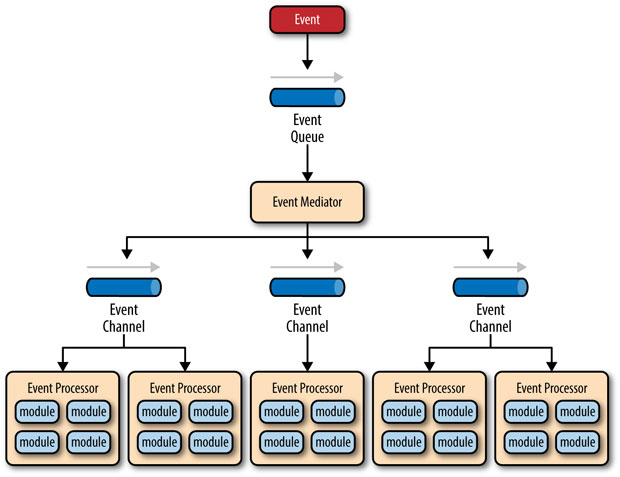
\includegraphics[width=0.9\columnwidth]{med-topology.jpg} 
    \caption{Schema Mediator Topology}
    \label{fig:eventdriver-med-top} 
\end{figure}

\paragraph{Mediatore di eventi}
Il mediatore (l’\emph{Event Mediator}) ha il compito di orchestrare i passi necessari per rispondere ad un evento iniziale; per ogni passo invia uno specifico evento di processamento ad un canale (\emph{Event Channel}). Il mediatore non applica nessun tipo di logica, conosce solo i passi necessari per gestire l’evento iniziale e quindi li genera.
\paragraph{Canale di eventi}
Si tratta generalmente di un canale di comunicazione asincrono. Questo può essere di due tipi:
\begin{itemize}
    \item coda di messaggi;
    \item topic di messaggi.
\end{itemize}
\paragraph{Esecutore di eventi}
Contiene la vera logica di business per processo ogni evento. Sono auto contenuti, indipendenti e scarsamente accoppiati.



\subsubsection{Broker topology}
In questo approccio non è presente un mediatore centrale. Il flusso dei messaggi viene distribuito dai vari esecutori, creando una catena di eventi che generano a loro volta altri eventi. Risulta molto utile nel caso in cui il flusso sia molto semplice. 

In questo approccio ci sono due principali componenti:
\begin{itemize}
    \item un \emph{broker} che contiene tutti i canali;
    \item vari esecutori di eventi.
\end{itemize}
    
In figura \ref{fig:eventdriven-bro-top} si riporta una generica architettura \emph{Event Driven Broker Topology}.

\begin{figure}[htbp]
    \centering
    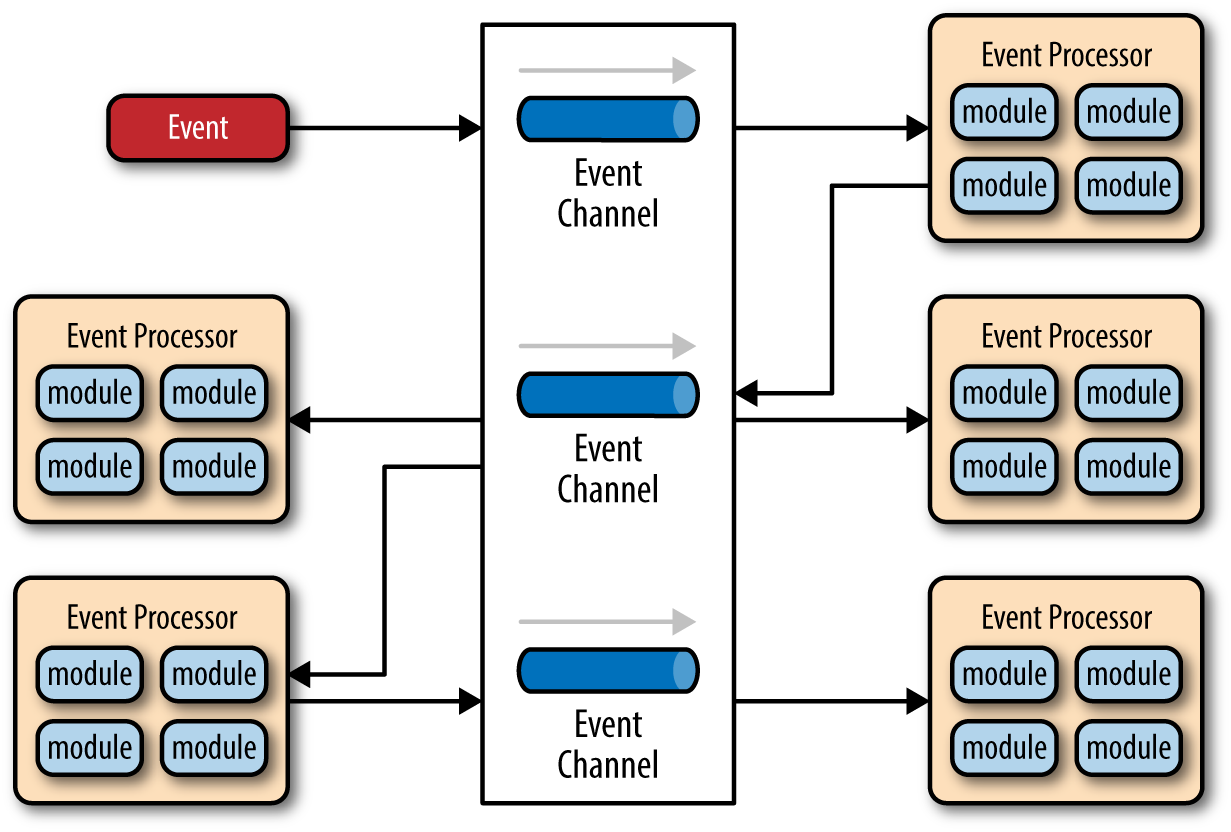
\includegraphics[width=0.9\columnwidth]{brok-top.png} 
    \caption{Schema Broker Topology}
    \label{fig:eventdriven-bro-top} 
\end{figure}

\subsubsection{Considerazioni}
Di seguito si evidenziano alcune vantaggi e svantaggi in maniera analitica \footnote{site:event-driven}:
\paragraph{Agilità generale}
I cambiamenti sono generalmente isolati e possono essere fatti velocemente con piccoli impatti.
\paragraph{Facilità di deploy}
È dovuta all’alto disaccoppiamento degli esecutori. Questa nota vale particolarmente per la tipologia \emph{Broker} in quanto non presenta il mediatore.
\paragraph{Testabilità}
Richiede strumenti specializzati per generare eventi, questo potrebbe rendere i test di sistema difficoltosi. I test di unità invece sono facilmente implementabili. 
\paragraph{Scalabilità}
La natura indipendente dei componenti rende facile scalare questi in base alle necessità permettendo così un \emph{tuning} delle risorse molto fine.
\paragraph{Facilità di sviluppo }
È il principale svantaggio di queste architettura.


Uno dei principali svantaggi di questo tipo di architettura è la complessità di implementazione, dovuta al fatto che operazioni sono completamente asincrone e concorrenti. Si è comunque ritenuta questa architettura nella sua variante \emph{Broker Topology} adatta allo scopo soprattutto per questioni di \emph{performance}, scalabilità e facilità di \emph{deploy}.

\subsection{Overview}
Come già detto l’applicazione sarà strutturata con una architettura \emph{Event Driven} di tipo \emph{Broker topology}, questo implica che la logica di funzionamento sia incapsulata nei vari passaggi tra le varie code.
Gli esecutori sono i seguenti cinque:
\begin{itemize}
    \item \textbf{Starter}: con il compito di ascoltare gli eventi iniziali dei vari RSP e di ricevere i vari dati ottenuti tramite codici QR;
    \item RetriveInfo: con il compito di ottenere le informazioni necessarie da \emph{Monokee};
    \item \textbf{PageResponce}: con il compito di generare e visualizzare le pagine nel broswer dell’utente, sia di fallimento che di comunicazione;
    \item \textbf{PiiDataHandler}: con il compito di verificare i dati nell’ITF e verificare che questi siano sufficienti per effettuare l’accesso;
    \item \textbf{RSPSendingWork}: con il compito di inviare al RSP le informazioni di accesso.
\end{itemize}
    
Gli eventi sono i seguenti:
\begin{itemize}
    \item \textbf{AccessRequest}: generato dallo \emph{Starter} e eseguito dal \emph{RetriveInfo};
    \item \textbf{PageResponce}: generato dal \emph{RetriveInfo} in caso di errore o per mostrare il lettore QR, dal \emph{PiiDataHandler} in caso di \emph{login} o in caso di insuccesso della verifica;
    \item \textbf{VerificationWork}: generato dallo \emph{Starter} per verificare i dati forniti tramite il QR e quelli forniti da \emph{RequireInfo} siano conformi e verificati; 
    \item \textbf{RSPSendingWork}: generato da \emph{PiiDataHandler} in caso di verifica positiva.
\end{itemize}
    
 Il diagramma in figura \ref{fig:eventdriven-flusso-code} rappresenta come i vari eventi di lavoro si distribuiscono tra i vari esecutori.

 \begin{figure}[!h]
    \centering
    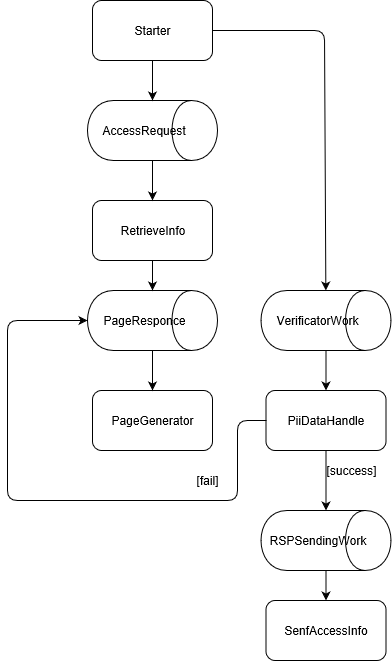
\includegraphics[width=0.7\columnwidth]{flow-eventi-sp.png} 
    \caption{Flusso eventi SP}
    \label{fig:eventdriven-flusso-code} 
\end{figure}
Lo \emph{Starter} quando riceve una richiesta d’accesso da parte del RSP procede a generare il lavoro di \emph{AccessRequest}, una volta ricavati tutti i dati necessari per l’accesso da \emph{Monokee}, viene affidato al \emph{PageResponce} l’incarico di visualizzare la pagina che richiede l’inserimento del QR. I dati verranno poi inseriti dall’utente e attraverso lo \emph{Starter} verrà creato un lavoro di verifica dei dati inseriti e se questi sono sufficienti ad accedere al servizio, tramite un’ulteriore accesso a \emph{Monokee}. In caso di esito positivo viene creato un lavoro di invio dati verso il RSP altrimenti verrà visualizzata una pagina di errore.
%**************************************************************

%**************************************************************
\newpage
\subsection{Progettazione}
\label{sec:progettazione}
In figura \ref{fig:sp-uml-diag} si presenta un diagramma delle classi che attua la gestione delle code sopra espletata. Il diagramma è stato redatto in formato \emph{UML 2.0}, con leggere modifiche relativo alla rappresentazione delle varie istanze del template \emph{CommandQueue}. Questo è stato fatto al fine di rendere più leggibile e comprensibile il diagramma. Come si può notare sono presenti componenti non presenti nella precedente trattazione. Questi servono per effettuare le comunicazioni con l’ambiente esterno. Si è deciso per questioni di semplicità di non creare code separate.

\begin{figure}[!htbp]
    \centering
    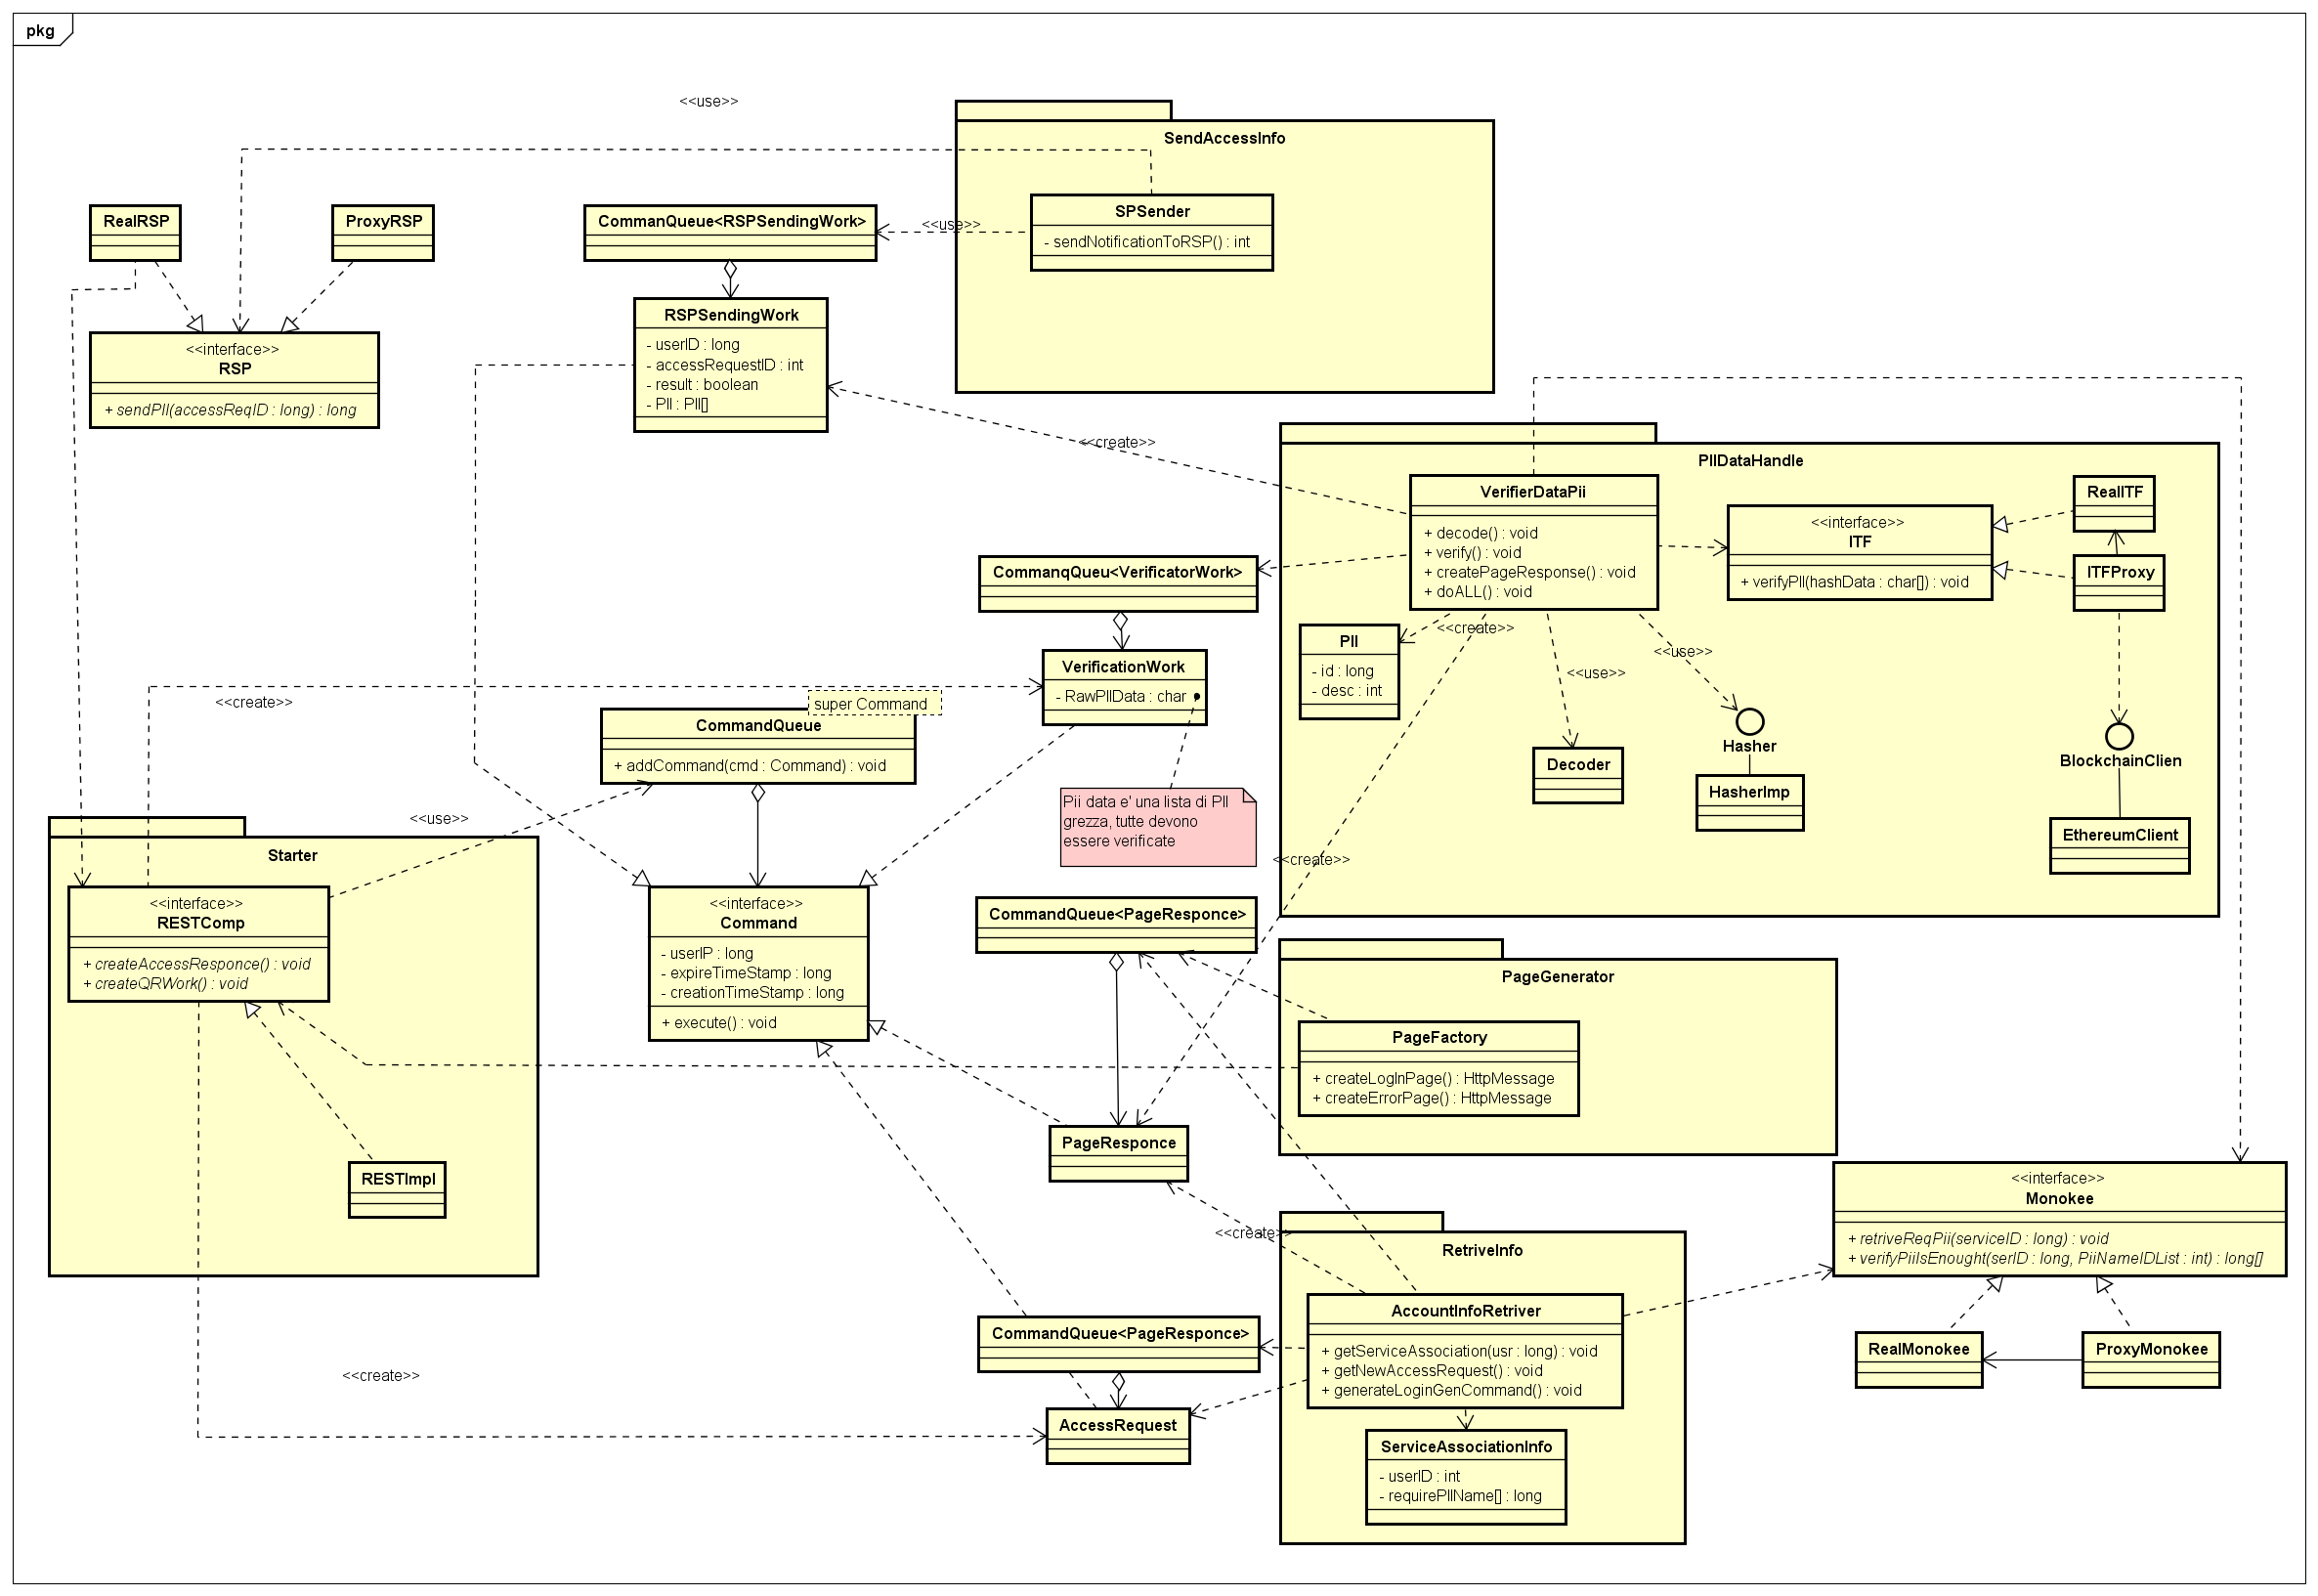
\includegraphics[width=0.9\columnwidth]{SPdiagram.png} 
    \caption{Diagramma delle classi del modulo SP}
    \label{fig:sp-uml-diag} 
\end{figure}

\subsubsection{Starter}
Lo \emph{Starter} rappresenta l’esecutore iniziale. Questo rimane in ascolto di eventuali richieste di accesso inoltrate dagli \emph{RSP} e da inizio all’esecuzione di questa. Riceve inoltre i dati provenienti dai codici QR. In figura \ref{fig:starter-uml-diag} viene riportato il diagramma UML dell'esecutore. Le classi più significative sono di seguito descritte.
\begin{figure}[htbp]
    \centering
    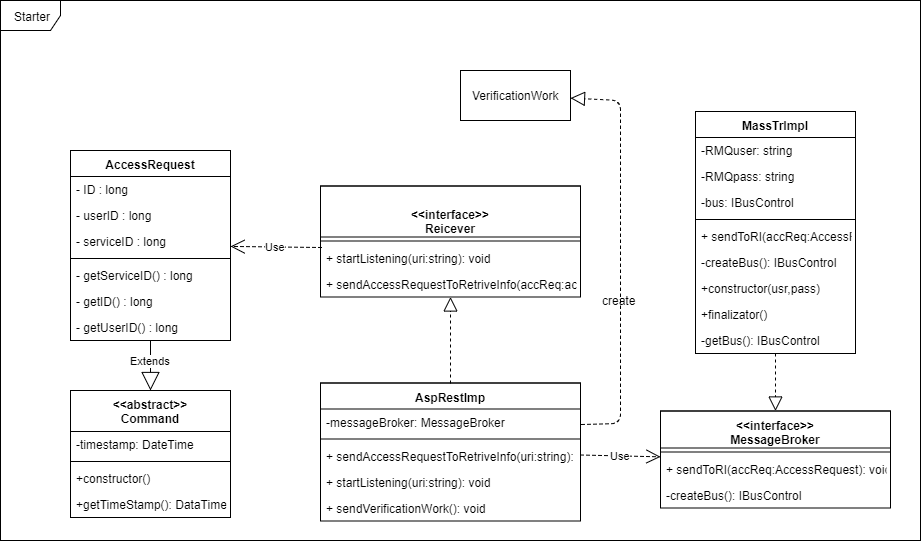
\includegraphics[width=0.9\columnwidth]{starter-uml.png} 
    \caption{Rappresentazione UML di \emph{Starter}}
    \label{fig:starter-uml-diag} 
\end{figure}
\begin{namespacedesc}
    \classdesc{Reicever}{è un'interfaccia con il compito di ricevere le comunicazioni provenienti dal sito di login e, quindi, inoltrare i messaggi alla coda successiva (\emph{RetrieveInfo}). Rappresenta il \emph{driver} del componente \emph{Starter}.}
    \classdesc{AspRestImpl}{è una possibile implementazione della strategia di comunicazione tramite \emph{REST}. Implementa l’interfaccia \emph{Reicever}.}
    \classdesc{MessageBroker}{è un'interfaccia con il compito di definire i metodi necessari alla gestione dalla rete di comunicazione \emph{RabbitMQ}.}
    \classdesc{MassTransitImpl}{questa classe implementa il MessageBroker utilizzano la libreria MassTransit.}
\end{namespacedesc}

\subsubsection{RetriveInfo}
È l’esecutore con il compito di ottenere le informazioni necessarie da \emph{Monokee}. In caso di associazione presente manda il lavoro di creazione pagina di login, in caso di associazione non presente manda il lavoro di creazione pagina di errore.
In figura \ref{fig:retrive-info-uml-diag} viene riportato il diagramma UML dell'esecutore. Le classi più significative sono di seguito descritte.
\begin{figure}[htbp]
    \centering
    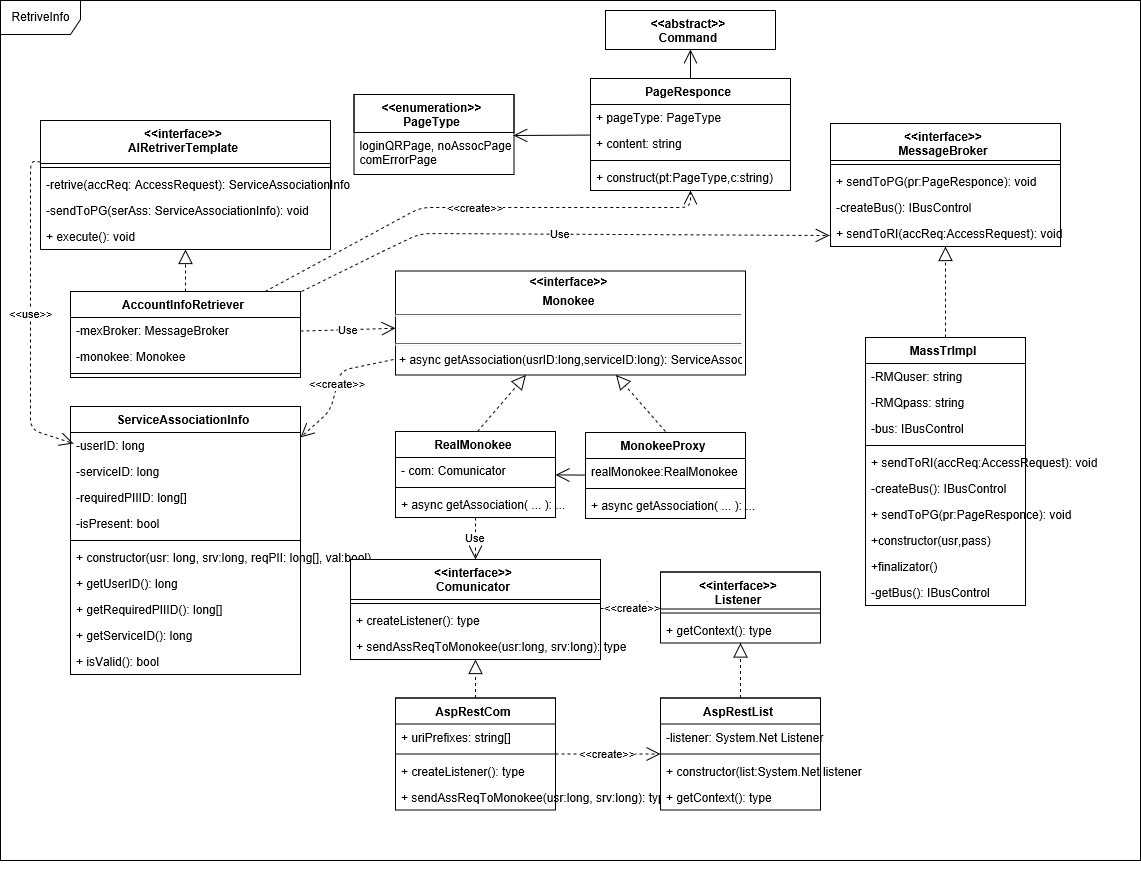
\includegraphics[width=0.9\columnwidth]{retrive-info-uml.png} 
    \caption{Rappresentazione UML di \emph{RetriveInfo}}
    \label{fig:retrive-info-uml-diag} 
\end{figure}
\begin{namespacedesc}
    \classdesc{AIRetriverTemplate}{questa interfaccia ha lo scopo di ricevere gestire e inoltrare i messaggi alla coda successiva (\emph{RetrieveInfo}). Rappresenta un template (\emph{Templete pattern}) del \emph{driver} dell’esecutore \emph{RetriveInfo}.}
    \classdesc{AccountInfoRetriever}{implementazione di \emph{AIRetriverTemplate}.}
    \classdesc{ServiceAssociationInfo}{questa classe rappresenta le informazioni ottenute da \emph{Monokee}, riporta i dati della \emph{AccessRequest} che l’ha generata e ci aggiunge l’informazione relativa alla lista delle \emph{PII} richieste e la presenta o meno della associazione in \emph{Monokee}. È un oggetto immutabile.}
    \classdesc{PageType}{Questo \emph{enumeration} definisce le varie possibili pagine creabili dall’esecutore \emph{PageGenerator}.
    I possibili tipi sono:
    \begin{itemize}
        \item loginQRPage: è una pagina mostra cattura il codice QR con le informazioni necessarie;
        \item noAssocPage: è una pagina che comunica che l’utente che ha effettuato una richiesta per un servizio a cui non è abilitato (non possiede l’associazione in Monokee);
        \item comErrorPage: è una pagina che comunica un generico errore di comunicazione.
    \end{itemize}}
    \classdesc{Monokee}{si tratta di un’interfaccia con il compito di fornire un’astrazione del servizio \emph{Monokee}. Questa interfaccia con \emph{RealMonokee} e \emph{ProxyMonokee} rappresenta un’applicazione del pattern \emph{Proxy}.}

    \classdesc{RealMonokee}{è una classe che rappresenta il reale oggetto \emph{Monokee}, questa classe poi dialoga con \emph{RESTComp} per ottenere i dati. Questa classe con \emph{RealMonokee} e \emph{ProxyMonokee} rappresenta un’applicazione del pattern \emph{Proxy}.}

    \classdesc{ProxyMonokee}{è una classe che rappresenta un \emph{proxy} dell’oggetto \emph{Monokee}, questa classe applica una politica di acquisizione pigra. Questa classe con \emph{RealMonokee} e \emph{ProxyMonokee} rappresenta un’applicazione del pattern \emph{Proxy}}

    \classdesc{Comunicator}{questa classe fornisce un’interfaccia per gestire tutte le informazioni attraverso fonti esterne. Deve essere usata per comunicare con \emph{Monokee} e il \emph{Real Service Provider}.}
    \classdesc{AspRestCom}{questa classe implementa \emph{Comunicator} tramite l'utilizzo della libreria \emph{Asp.NET}.}

    \classdesc{Listener}{È un'interfaccia con il compito di rimanere in ascolto su determinati \emph{uri}. È un oggetto non mutabile.}
    \classdesc{AspRestList}{È un oggetto con il compito di rimanere in ascolto su determinati \emph{uri}. È un oggetto non mutabile. Questa classe è un \emph{wrapper} del \emph{listener} di \emph{System.Net}. Implementa \emph{Listener}.}
\end{namespacedesc}


\subsubsection{PageGenerator}
È l’esecutore con il compito di ascoltare le richieste di creazione pagina provenienti dagli altri esecutori e quindi di generarle come richiesto e di inviarle al \emph{browser}del richiedente. In figura \ref{fig:pagegenerator-uml-diag} viene riportato il diagramma UML dell'esecutore. Le classi più significative sono di seguito descritte.
\begin{figure}[htbp]
    \centering
    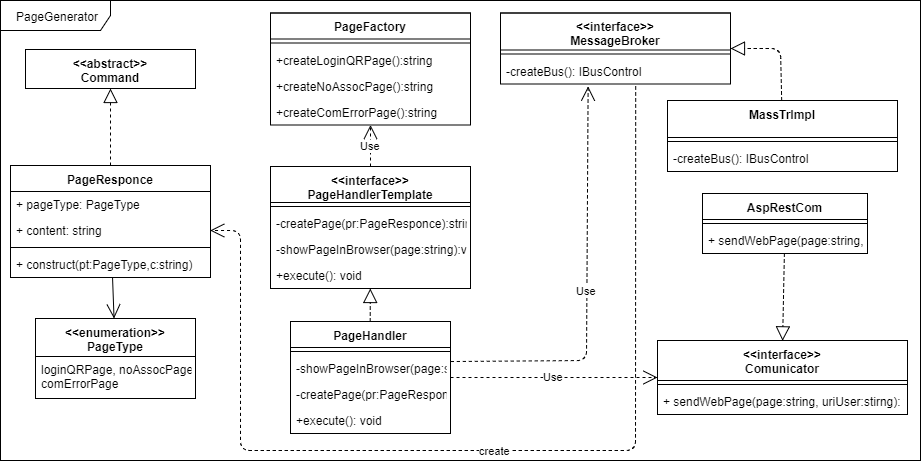
\includegraphics[width=0.9\columnwidth]{pagegenerator-uml.png} 
    \caption{Rappresentazione UML di \emph{PageGenerator}}
    \label{fig:pagegenerator-uml-diag} 
\end{figure}
\begin{namespacedesc}
    \classdesc{PageHandlerTemplate}{questa interfaccia consiste in un \emph{template} per la creazione di un \emph{driver} per la gestione e l’esecuzione dei \emph{Command} di \emph{PageGenerator}.}
    \classdesc{PageHandler}{Questa classe implementa la struttura fornita da \emph{PageHandlerTemplate}.}
\end{namespacedesc}

\subsubsection{PIIDataHandler}
Questo esecutore ha il compito di ricevere nella propria coda dallo \emph{Starter} una serie di lavori di verifica e quindi di verificare questi sia verso \emph{Monokee} sia verso l’\emph{ITF}. In questo esecutore sono presenti le interfacce \emph{Command}, \emph{Monokee} e \emph{MessageBroker} che non verranno presentate. In figura \ref{fig:piidatahandler-diag} viene riportato il diagramma UML dell'esecutore. Le classi più significative sono di seguito descritte. 
\begin{figure}[htbp]
    \centering
    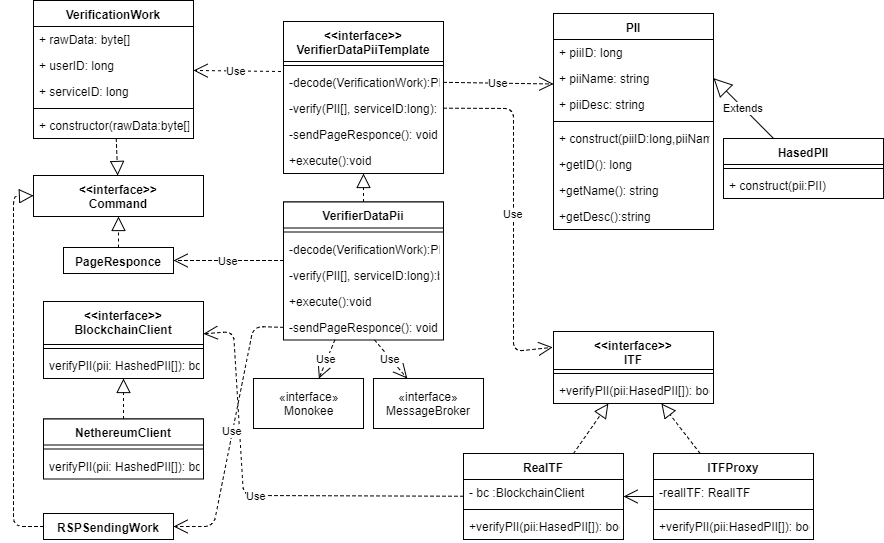
\includegraphics[width=0.9\columnwidth]{piidatahandler-uml.png} 
    \caption{Rappresentazione UML di \emph{PIIDataHandler}}
    \label{fig:piidatahandler-uml-diag} 
\end{figure}

\begin{namespacedesc}
    \classdesc{VerificationDataPiiTemplate}{questa interfaccia rappresenta il \emph{template} da seguire per eseguire l’algoritmo di gestione di un \emph{VerificationPiiWork}. Dalla ricezione fino al suo esaurimento.}
    \classdesc{VerificationDataPii}{Questa classe rappresenta un’applicazione del \emph{template} da seguire per eseguire l’algoritmo di gestione di un \emph{VerificationPiiWork}. Dalla ricezione fino al suo esaurimento.}
    \classdesc{PII}{è una classe che rappresenta una PII. Contiene l’id, la descrizione di una PII.}
    \classdesc{HashedPII}{questa classe rappresenta una \emph{PII} con le informazioni \emph{piiName} e \emph{piiDesc} sotto forma di \emph{Hash}, questa classe dev’essere usata per comunicare con l’\emph{ITF}. L’oggetto è immutabile.}
    \classdesc{ITF}{si tratta di un’interfaccia con il compito di fornire un’astrazione del componente ITF. Questa interfaccia con \emph{RealITF} e \emph{ProxyITF} rappresenta un’applicazione del pattern \emph{Proxy}.}

    \classdesc{RealITF}{è una classe che rappresenta il reale oggetto ITF, questa classe poi dialoga con il \emph{BlockchainClient} per ottenere i dati. Questa classe con \emph{RealITF} e \emph{ProxyITF} rappresenta un’applicazione del pattern \emph{Proxy}.}

    \classdesc{ITFProxy}{è una classe che rappresenta un \emph{proxy} dell’oggetto ITF, questa classe applica una politica di acquisizione remota. Questa classe con \emph{RealITF} e \emph{ITFProxy} rappresenta un’applicazione del pattern \emph{Proxy}.}

    \classdesc{BlockchainClient}{questa interfaccia ha il compito di rappresentare un canale di comunicazione verso gli \gls{SmartContractg}. Deve essere atea rispetto alla tipologia di \gls{blockchaing} usata.}

    \classdesc{NethereumClient}{Questa classe rappresentare un canale di comunicazione verso gli \gls{SmartContractg} di una rete \emph{Ethereum}. Fa uso della libreria \emph{.NET Nethereum} per instaurare la comunicazione. }
\end{namespacedesc}

\subsubsection{SendAccessInfo}
Questo esecutore ha il compito di inviare le informazioni necessarie per effettuare il \emph{login} al \emph{RSP} ed al \emph{back-end} di \emph{Monokee}. Queste informazione deve essere fornite in forma non di \emph{hash}. I \emph{Command} provengono da \emph{PIIDataHandle}. In figura \ref{fig:sendaccessinfo-diag} viene riportato il diagramma UML dell'esecutore. Le classi più significative sono di seguito descritte.

\begin{figure}[htbp]
    \centering
    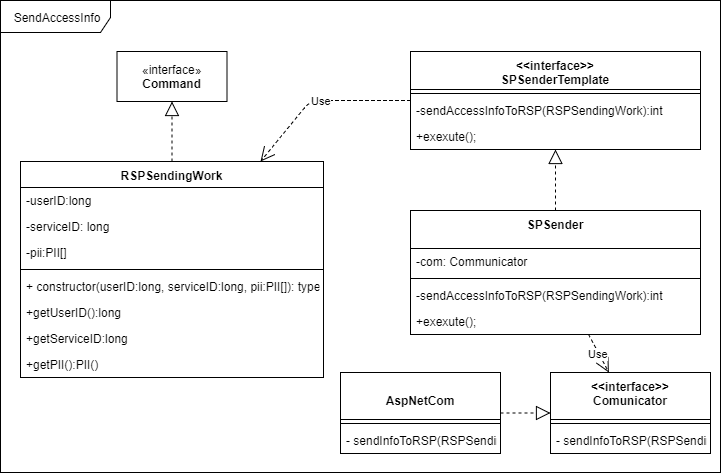
\includegraphics[width=0.9\columnwidth]{SendAccessInfo.png} 
    \caption{Rappresentazione UML di \emph{SendAccessInfo}}
    \label{fig:sendaccessinfo-uml-diag} 
\end{figure}

\begin{namespacedesc}
    \classdesc{RSPSenderTemplate}{questa interfaccia rappresenta il \emph{template} da seguire per eseguire il lavoro dell’esecutore. In altre parole rappresenta l’algoritmo da eseguire per espletare il lavoro di invio attributi al \emph{RSP}.}
    \classdesc{RSPSender}{questa classe implementa il \emph{template} da seguire per eseguire il lavoro dell’esecutore. In altre parole rappresenta l’algoritmo da eseguire per espletare il lavoro di invio attributi al \emph{RSP}.}
\end{namespacedesc}

\paragraph{CommonElement}
Questo componente contiene una serie di elementi usati da più esecutori, primi fra tutti gli oggetti \emph{Command}. Pertanto si è deciso di creare una libreria condivisa tra i vari esecutori.
Le classi più significative sono di seguito descritte.
 
\begin{namespacedesc}

    \classdesc{Command}{È una classe che rappresenta un generico evento nel contesto dell’architettura \emph{event driven}. Questa interfaccia viene poi implementata da:
    \begin{itemize}
        \item \textbf{AccessRequest}: generato dallo \emph{Starter} e eseguito dal \emph{RetriveInfo}, rappresenta il lavoro per gestire la richiesta di accesso;
        \item \textbf{PageResponce}: generato dal \emph{RetriveInfo} in caso di errore o per mostrare il lettore QR, dal \emph{PiiDataHandler} in caso di \emph{login} o in caso di insuccesso della verifica. Rappresenta il lavoro di generazione e sottomissione delle pagine all’utente;
        \item \textbf{VerificationWork}: generato dallo \emph{Starter} per verificare i dati forniti tramite il QR e quelli forniti da \emph{Monokee} siano conformi e verificati; 
        \item \textbf{RSPSendingWork}: generato da \emph{PiiDataHandler} in caso di verifica positiva. Rappresenta il lavoro di sottomissione dati in caso di verifica positiva.
    \end{itemize}
    }

    \classdesc{Hasher}{È un’interfaccia che ha il compito di eseguire l’\emph{hash} di un dato. Rappresenta un’applicazione dello \emph{strategy pattern}. }

    \classdesc{HasherImpl}{È una classe che implementa un’implementazione della classe \emph{Hasher}. Esegue l’\emph{hash} di un dato. Rappresenta con \emph{Hasher} un’applicazione dello \emph{strategy pattern}.}

\end{namespacedesc}


%**************************************************************
\subsection{Design Pattern utilizzati}
Al fine di garantire elevate doti di qualità e manutenibilità dell’architettura sono stati usati una serie di design pattern. Di seguito segue una breve descrizione di questi.


\paragraph{Command Pattern} permette di isolare la porzione di codice che effettua un'azione (eventualmente molto complessa) dal codice che ne richiede l'esecuzione; l'azione è incapsulata nell'oggetto \emph{Command}. 
\paragraph{Remote Proxy} fornisce una rappresentazione locale di un oggetto remoto remote. 
\paragraph{Strategy Pattern} è un oggetto che permette di separare l’esecuzione di un metodo dalla classe che lo contiene. Usando un’interfaccia per astrarre il metodo è poi possibile crearne molteplici implementazioni. Questo è risultato molto utile nel contesto di un’applicazione multi piattaforma in cui alcune procedure andavano implementate in nativo. Oltre all’appena citato vantaggio questo ha reso possibile separare il metodo dall’implementazione. 
\paragraph{Dependency Injection} è un pattern che permette di delegare il controllo della creazione oggetti ad un oggetto esterno. Questo permette di semplificare la gestione delle dipendenze e nel contesto dello \emph{strategy pattern} permette di inoculare l’implementazione corretta. 
\paragraph{Factory Method} è un pattern che permette di convogliare tutte le funzioni di creazione di vari elementi ad un oggetto unico. 

%**************************************************************
\section{Implementazione}

Le attività di implementazione e codifica sono state la parte di maggior impegno e sforzo dell'intero progetto. Hanno occupato in termini orari 120 ore, le quali rappresentano quasi il 40\% della durata del progetto. Esse hanno fatto emergere diversi errori di progettazione e di codifica, inoltre ci sono stati diverse ripensamenti da parte dell'azienda che hanno portato a riprogettare interi moduli. Nei paragrafi seguenti si cercherà di presentare le implementazioni più significative all'interno del progetto.

\subsection{Procedura di login}
L'applicativo mobile non prevedeva una gestione degli account propria, ma utilizzava gli account già presenti nel sistema \emph{Monokee}. Questo ha necessitato quindi la codifica di un apposita procedura di \emph{login} in modo di autenticare un utente in base ad una coppia di valori \emph{email} e \emph{password}. 

La suddetta procedura consiste principalmente in due chiamate HTTPS, la prima con lo scopo di ottenere l'id dell'utente tramite la mail fornita, la seconda allo scopo di verificare se la \emph{password} sia conforne all'id ottenuto dalla prima chiamata. 

La prima fase era attuata da un metodo chiamato \textbf{Task<string> RetriveUserID(string usr)}. Questo metodo inviava tramite una POST il seguente \emph{json}, con il quale forniva le informazioni necessarie ad ottenere l'id :

\begin{lstlisting}[caption={Json della prima request di login}]
    {
        email = "user@dominio.com",
        mobile = "false",
    }
\end{lstlisting}

La risposta doveva invece seguire il seguente schema:

\begin{lstlisting}[caption={Json risposta user\_id}]
    {
        success = "true",
        message = "ok",
        user_id = "df3c92kzz1",
    }
\end{lstlisting}

La risposta in alcuni casi poteva presentare altri campi dati, ma questi venivano ignorati dall'applicativo. Risposte che non presentavano le precedentemente citate tre informazione o che non riportavano i valori "true" ed "ok" rispettivamente su "success" e "message" causavano il lancio di un'eccezzione che faceva comparire un messaggio di fallimento a schermo.

Una volta ottenuto il valore "user\_id" si procedeva alla verifica della password col metodo
\textbf{getTokenID(string userId, string password)}.
Questo avveniva sempre tramite l'uso di una comunicazione POST. Nella request veniva mandato il seguente \emph{json}:

\begin{lstlisting}[caption={Json richiesta token}]
    {
        user_id = "df3c92kzz1",
        password = "Passw0rd",
        mobile = "false",
        persistence = "false",
        cc_key = "key",
        salt = "salt",
        domain_id = "5b475bd150e783334b5bb861",
    }
\end{lstlisting}

Il campo "persistence" è utile alla gestione interna del dato e non rientra in nessun modo nel progetto.
I parametri "\emph{cc\_keys}" e "\emph{salt}" invece sono due valori tipici delle procedure di \emph{login}. Questi servono a rendere più complessi gli attacchi a dizionario verso il sistema, infatti i due valori per essere generati richiedono un elevato onere computazionale sia in termini di spazio che di tempo, in quanto devono rispettare delle determinate condizioni. La codifica del codice per generare questi due valori ha richiesto innumerevoli sforzi e si è rivelata essere non banale.
L'applicativo \emph{Monokee} ha la caratteristica di offrire ai propri utenti domini seperati, un tipico utilizzo di questi è per esempio il dominio aziendale e quello personale. Il "\emph{domain\_id}" fornito da rappresenta il dominio personale. L'applicativo per ragioni di semplicità faceva l'accesso sempre allo stesso dominio. 

La risposta doveva seguire il seguente schema:
\begin{lstlisting}[caption={Json risposta token}]
    {
        success = "true",
        message = "ok",
        token = "qrdj99d7f9da0b2nf93Kd9LL"
    }
\end{lstlisting}

Il significato di "success" e "message" rimane analogo a quello precedentemente descritto, mentre il valore "\emph{token}" rappresenta un codice da inserire nell'\emph{header} sotto il nome di "\emph{Authorization}" nelle successive chiamata in modo tale da essere risposto. Questo codice ha validità di 24 ore, al seguito delle quali scade ed è necessario rieffettuare la procedura di \emph{login}. Risulta estremamente importante al momento del \emph{logout} rimuovere dall'\emph{header} il \emph{token}, in quando una successiva operazione di \emph{login} ne avrebbe aggiunto un altro causando un doppio \emph{token}. Questo avrebbe fatto fallire le successive richiesta, seppur consentendo l'accesso.

Per ragioni progettuali interne a \emph{Monokee} le chiamate se ricevute vengono sempre risposte con uno \emph{status code} 200, a prescindere del fatto che queste siano accettate o rifiutate. Per questa ragione al fine di sostituire i vari codici di errore vengono usati i campi "success" e "message". 

La codifica di questa procedura non ha presentato particolari difficolta se non quella della generazione del \emph{cc\_key} e del \emph{salt}. 

\subsection{Uso del database SQLite}

Nel contesto dell'applicazione mobile per effettuare la persistenza dei dati si è deciso di utilizzare una base di dati relazionale. La scelta è ricaduta su \emph{SQLite}. Si è deciso di operare con questa base di dati utilizzando il design pattern \emph{data access object} e apposite libreria di sistema che lo implementavano, questa pratica si è rivelata essere molto pratica ed efficace ai fini del progetto. Ovviamente risulta limitata comparata rispetto all'uso del codice \emph{sql}, ma le necessità applicative non richiedevano simili finezze.

A titolo di esempio si discute ora della memorizzazione di un PII.

\begin{lstlisting}[caption={codice creazione DAO}]
    public DBDao()
    {
        database = DependencyService
            .Get<ILocalDataProvider>()
            .GetConnection();
        database.CreateTable<PIIModel>();
        database.CreateTable<UserModel>();
    }
\end{lstlisting}

Il codice appena presentato rappresenta la creazione dell'oggetto che fornisce l'accesso alla base di dati, come si può notare il corpo del costrutture crea una connessione tramite l'uso di \emph{DependencyService}, successivamente crea le tabelle. Ovviamente in caso le tabelle siano già presenti, le istruzioni non alterano la base di dati. 

A differenza di quanto uno si potrebbe aspettare, la funzione \emph{CreateTable} non richiede informazione sui tipi di dato e/o sulle colonne da creare. Queste informazione vengono dedotte dal tipo che gli viene fornito, il quale andrà a rappresentare il modello di una tupla della tabella.

Si propone adesso il codice di \emph{PIIModel}:
\begin{lstlisting}[caption={codice PIIModel}]
    [Table("PIIModel")]
    public class PIIModel
    {
 
        [PrimaryKey, AutoIncrement]
        public int Id;
        
        [Indexed(Name = "nameId", Order = 1, Unique = true)]
        public string UserID;

        [Indexed(Name = "nameId", Order = 2, Unique = true)]
        public string Name;
        [NotNull]

        //continua ...
\end{lstlisting}

I campi dati pubblici vengono considerati come i valori delle colonne, mentre altre informazioni necessarie vengono fornite tra parentesi quadre. Queste sono per esempio le chiavi, i valori non nulli, i vincoli di integrità, il nome della tabella etc...

Sequendo questa tecnica la gestione del database risulta particolarmente semplice. Vengono ora riportati degli esempi di codice per l'inserimento e la rimozione di una PII dalla base di dati:

\begin{lstlisting}[caption={codice aggiunta e rimozione PIIModel}]
public int AddPII(PIIModel pii)
    {
        lock (collisionLock)
        {
            if (pii.Id != 0)
            {
                database.Update(pii);
                return pii.Id;
            }
            else return database.Insert(pii);      
        }
    }

public int DeletePII(int piiID)
{
    lock(collisionLock)
    {
        return database.Delete<PIIModel>(piiID);
    }
}
\end{lstlisting}

Ovviamente interrogazioni più complicate risultano non essere possibile tramite funzioni di libreria, per queste particolari occassioni si è dovuto utilizzare del codice \emph{sql}.

\begin{lstlisting}[caption={Esempio di query sql}]
public List<PIIModel> GetPIIs(string name, string user\_id)
    {
        lock (collisionLock)
        {
            return (from i in database.Table<PIIModel>()
                    where (i.Name == name && i.UserID==user\_id)
                    select i).ToList();
        }
    }
\end{lstlisting}

L'uso di queste tecniche e dei modelli ha permesso di limitare al massimo l'utilizzo di codice \emph{sql}, inoltre ha permesso una più facile gestione del dato in quanto la risposta ad una \emph{query} veniva già presentata in forma di oggetto.

\subsection{Implementazione del databinding}
L'applicaione mobile richiedeva la creazione di molteplici schermate che dovevano sempre rimanenere aggiornare rispetto ad un particolare oggetto e viceversa. Questo risultava particolarmente importante in quanto era fondamentale che l’interfaccia fosse ben separata dalla logica di \emph{business}, affinché una modifica nella logica o nel modello di dominio non si rifletta sull’interfaccia. 

A questi scopi \emph{Xamarin} offre la cosidetta tecnica del \emph{databinding} tra intefaccia e oggetto. Ora si ripropone l'oggetto \emph{PIIModel}, questa volta però non omettendo il codice necessario per il \emph{databinding}.

\begin{lstlisting}[caption={esempio di oggetto in databinding}]
[Table("PIIModel")]
public class PIIModel : INotifyPropertyChanged
{
    private int piiID;
    [PrimaryKey, AutoIncrement]
    public int Id
    {
        get { return piiID; }
        set {
            piiID = value;
            OnPropertyChanged(nameof(Id));
        }
    }

    \\altro codice ommesso ...

    private void OnPropertyChanged(string propertyName)
    {
            PropertyChanged?.Invoke(this,
            new PropertyChangedEventArgs(propertyName));
    }
}
\end{lstlisting}

Come si può notare per poter effettuare il \emph{databinding} è necessario che la classe \emph{PIIModel} implementi l’interfaccia \emph{INotifyPropertyChanged}, che definisce l’evento \emph{PropertyChanged} di tipo \emph{PropertyChangedEventHandler}. Questo evento prende un’istanza della classe \emph{PropertyChangedEventArgs} che definisce la proprietà \emph{PropertyName} di tipo \emph{string}, attraverso la quale è possibile sapere quale proprietà nell'oggetto \emph{PIIModel} è cambiata (permettendo all’evento di accedere a quella proprietà).

Attraverso la proprietà pubblica \emph{Id}, offriamo la possibilità lato codice di ottenere le informazioni sul valore corrente attraverso il \emph{get}, e di impostare un nuovo valore per tale proprietà attraverso il \emph{set} ogni qualvolta il valore assunto dalla variabile \emph{name} differisce da quella corrente. Proprio in quest’ultima porzione viene richiamato il metodo \emph{OnPropertyChanged}, che prenderà in ingresso il nome della proprietà che deve essere aggiornata innescando il meccanismo sopra descritto. 

Per effettuare l'effettiva collegamento basta inserire nel codice che gestische la schermata la seguente istruzione:
\begin{lstlisting}[caption={codice di connessione}]
    BindingContext = PIIModel;
\end{lstlisting}

Questo renderà possibile nel codice grafico (XAML) di poter utilizzare i valori dell'oggetto. Di seguito viene mostrato un esempio:

\begin{lstlisting}[caption={esempio di vista che usa il databinding}]
<?xml version="1.0" encoding="utf-8" ?>
<ContentPage xmlns="http://xamarin.com/schemas/2014/forms"
             xmlns:x="http://schemas.microsoft.com/winfx/2009/xaml"
             x:Class="IdentityWallet.PIIVisualizerPage"
             Title="{Binding Name}">
    <ContentPage.Content>
        <ScrollView>
            <StackLayout VerticalOptions="StartAndExpand" Padding="20">
                <Label Text="Id"/>
                <Label x:Name="piiID" Text="{Binding Id}"/>
            
                <Label Text="Name" />
                <Entry x:Name="piiName" Text="{Binding Name}"/>
            
                <- altro codice ->
            </StackLayout>
        </ScrollView>
    </ContentPage.Content>
</ContentPage>
\end{lstlisting}

\subsection{Instaurazione della rete di messaggi}
Il modulo SP è composto da diversi componenti, i quali sono residenti in programmi differenti e seperati fra loro. L'unico modo di comunicazione che utilizzano è un \gls{messagebrokerg}\glsfirstoccur di nome \emph{RabbitMQ}. Questo deve essere eseguito su un server e verrà utilizzato dai vari componenti tramite il suo \emph{uri}.
L'applicativo richiede che nel server sia installato \emph{Erlang}. Una volta averlo installato si può procedere all'installazione di \emph{RabbitMQ} seguendo la guida presente al seguente url \url{https://www.rabbitmq.com/download.html}. Per eseguire correttamente le funzionalità del modulo SP è inoltre necessario creare una rete col nome di "test"; per fare questo è necessario abilitare l'interfaccia di configurazione di \emph{RabbitMQ} seguendo la seguente guida \url{https://www.rabbitmq.com/management.html}.
Una volta abilitata l'interfaccia questa sarà disponibile al seguente indirizzo \url{http://localhost:15672/#/connections}. La pagina che si presenterà avrà una scheda chiamata "network" dalla quale sarà possibile aggiungere la rete di nome "test".
Fatto questa la configurazione di \emph{RabbitMQ} è terminata; ora basta avviare il \emph{broker} tramite terminale usando il comando \emph{rabbitmq-server start}.


\subsection{Gestione delle code e dei messaggi}
Come già discusso il modulo SP ha un'architettura del tipo \emph{even driven}. L'applicazione di tale libreria ha necessitato dell'uso di una libreria per la gestione e l'invio dei vari messaggi.

Il modulo SP è diviso in molteplici esecutori ognuno del quale presenta del codice per la gestione dei messaggi equivalente, a titolo di esempio si procede ad esporre l'esecutore \emph{ITFVerifier}.

All'avvio l'esecutore ha il compito di creare un oggetto in grado di individuare la rete che gestisce i messaggi (questa era disponibile all'uri definito in \emph{GeneralSetting.RabbitMQHost}) e quindi effettuare il collegamento ad essa tramite la sottomissione di una coppia \emph{username}, \emph{password}.
Successivamente era necessario definire cosa doveva essere fatto dei messaggi in arrivo e sopratutto quale tipo di messaggi dovessero essere ascoltati. La parte finale del codice propostro mostra le instruzione necessarie a fare quanto appena detto. Tramite \emph{ReceiveEndpoint} viene stabilito il nome della coda dove verranno inseriti i messaggi catturati e il comportamento da intraprendere per ognuno di questi messaggi. Come comportarsi viene definito tramite una \emph{arrow function} che instanzia un \emph{Consumer} con un tipo da noi definito (\emph{VerificationWorkConsumer}). I messaggi da inserire nella code di ricezione non vengono decisi in base ad un'indicazione del mandante, ma tramite il tipo dell'oggetto che viene implementato da \emph{VerificationWorkConsumer}.
L'ultimi riga ha lo scopo di eseguire il lavoro in modalità asincrona.
\begin{lstlisting}[caption={creazione di un collegamento a \emph{RabbitMQ}}]
    _busControl = Bus.Factory.CreateUsingRabbitMq(x =>
        {
            IRabbitMqHost host = x.Host(new Uri(GeneralSetting.RabbitMQHost), h =>
            {
                h.Username("guest");
                h.Password("guest");
            });
            
            x.ReceiveEndpoint(host, "VerQueue",
                e => { e.Consumer<VerificationWorkConsumer>(); });
            
        });

        TaskUtil.Await(() => _busControl.StartAsync());
\end{lstlisting}

Adesso risulta utile analizzare il codice del \emph{Consumer}. Come si può notare la classe implementa \emph{IVerificationWork}, pertando nella coda che porta il nome di "VerQueue" verranno inseriti solo i messaggi che hanno come tipo \emph{IVerificationWork}.
Unico metodo implementabile è \emph{Consume} il quale rappresenta il codice da effettuare.

\begin{lstlisting}[caption={esempio di \emph{Consumer}}]
public class VerificationWorkConsumer : IConsumer<IVerificationWork>
{
    public async Task Consume(ConsumeContext<IVerificationWork> context)
    {
            //operazioni da effettuare

    }
}
\end{lstlisting}

Andiamo ora a vedere come si invia un messaggio un \emph{VerificationWork}:
\begin{lstlisting}[caption={codice invio di un messaggio}]
    public async Task SendToVerificationAsync(IVerificationWork verWork)
    {
        await _busControl.Publish(verWork);
    }
\end{lstlisting}

Come potete vedere questo avviene tramite la funzione \emph{Publish} dell'oggetto \emph{\_busControl}.

\subsection{Interazioni con la \emph{blockchain}}

Sia l'applicativo mobile IW, che l'applicativo server SP hanno previsto l'uso della stessa libreria \emph{Nethereum} al fine di effettuare le necessarie chiamate alla \emph{blockchain Ethereum}.
Questa libreria implementa il protocollo Ethereum\footcite{site:ethereum-yellow-paper} in ambiente \emph{.NET}.

Il protocollo discerne tra due tipi di chiamate, quelle in \textbf{sola lettura} e quella \textbf{in scrittura}; le prime sono identificate dai modificatori \emph{pure} o \emph{view}.

Le chiamate in sola lettura sono immediate e non richiedono l'esecuzione di una transazione, per queste ragioni hanno prestazione paragonabile a quelle di un linguaggio tradizionale e non richiedono le venga fornito dell'\gls{etherg}.

Le seconde invece, dovendo modificare la \gls{blockchaing}, hanno bisogno di effettuare una transazione con la conseguente esecuzione dell'algoritmo di consenso descritto nel capitolo \ref{cap:alg-cons}. Questo porta ai problemi di prestazioni e costo descritti in \ref{cap:prestazioni}

Prima di poter procedere a qualsiasi operazione era necessario creare un collegamente alla rete \emph{Ethereum} usata (nel nostro caso una rete locale all'azienda). Il sequente codice mostra le istruzioni necessarie.

\begin{lstlisting}[caption={Connessione alla rete di test},label={lst:connessione},language={C}]
account = new Account(GeneralSetting.accountPrivKey);
web3 = new Web3(account, blockchain_address);
\end{lstlisting}

La variabile \emph{web3} è l'oggetto che rappresenta la connessione. Il primo parametro del costruttore non è strettamente necessario, ma stabilisce un \emph{account} di default con il quale verranno pagate le transazioni. Si è deciso in fase di codifica di non minare direttamente le aggiunte di blocchi, ma di pagare la transazione. Per essere riconosciuti dalla rete è sufficiente fornire la chiave privata. 
\medskip

Ora è necessario richiamare un contratto presente nella rete. Per fare questo necessitiamo di due informazione: l'\textbf{indirizzo} e l'\gls{abig}\glsfirstoccur. L'\emph{ABI} di un contratto consiste in un \emph{json} contenente la definizione di tutti i metodi presenti nel contratto. Nel frammento ~\ref{lst:abi_ex} si mostra l'\emph{ABI} della chiamata che andremo ad effettuare, invece nel frammento ~\ref{lst:creazioneContr} si mostra la creazione dell'oggetto contratto. Dal contratto poi si ottiene la funzione.

\begin{lstlisting}[caption={Esempio di ABI},label={lst:abi_ex},language={C}]
[
    {
        "anonymous": false,
        "inputs": [
            {
                "indexed": true,
                "name": "_PII_ID",
                "type": "string"
            },
            {
                "indexed": false,
                "name": "result",
                "type": "bool"
            }
        ],
        "name": "eventResponse",
        "type": "event"
    },
    {
        "constant": false,
        "inputs": [
            {
                "name": "_publicKey",
                "type": "string"
            },
            {
                "name": "_PII_ID",
                "type": "string"
            },
            {
                "name": "_name",
                "type": "string"
            },
            {
                "name": "_description",
                "type": "string"
            }
        ],
        "name": "verify",
        "outputs": [
            {
                "name": "",
                "type": "bool"
            }
        ],
        "payable": false,
        "stateMutability": "nonpayable",
        "type": "function"
    }
]  
\end{lstlisting}

\begin{lstlisting}[caption={Creazione del contratto},label={lst:creazioneContr},language={[Sharp]C}]
    SPFContract = web3.Eth.GetContract(abi,
                "contract_address");
    var verifyFunction = SPFContract.GetFunction("verify");
\end{lstlisting}

Una volta ottenuto l'oggetto \emph{verifyFunction} non ci resta che effettuare la chiamata. Il metodo \emph{verify} effettua modifiche, quindi è necessario effettuare una transazione. La funzione \emph{SendTransactionAndWaitForReceiptAsync} effettua la chiamata del metodo \emph{Solidity} \emph{verify} e aspetta che questa fallisca o abbia successo. Una transazione non restituisce mai il risultato della chiamata, ma una ricevuta che ne attesta la riuscita o il fallimento. Per ottenere il risultato bisogna usare i cosidetti \emph{eventi} che vanno lanciati dal codice \emph{Solidity} con il contenuto del valore di ritorno. Gli eventi sono comunicati in \emph{broadcast} a tutti gli utenti connessi alla rete, di conseguenza ottenere il risultato richiede una serie di procedure particolari. La seconda parte del codice nel frammento \ref{lst:transax} mostra il codice necessario per filtrare gli eventi in base alla ricevuta e quindi ottenere il valore. 


\begin{lstlisting}[caption={Creazione del contratto},label={lst:transax},language={[Sharp]C}]
receipt = await verifyFunction.SendTransactionAndWaitForReceiptAsync(
    "account_address,
    null, 
    ITFID,
    description, 
    publicKeyBytes)
    .ConfigureAwait(false);          

    //CODICE PER GESTIRE L'EVENTO DI RISPOSTA
    var verifyEvent = SPFContract.GetEvent("eventResponse");
    var filterOnITFID = verifyEvent.CreateFilterInput(
        new BlockParameter(receipt.BlockNumber),
            BlockParameter.CreateLatest());
    var log = await verifyEvent.GetAllChanges<VerificationEvent>(filterOnITFID);
    result = log[0].Event.Result;
\end{lstlisting}


Le chiamate a metodi \emph{Solidity} detti \emph{puri}, invece, sono più semplici e restituiscono direttamente il risultato.
Di seguito un esempio di una chiamata di questo tipo.

\begin{lstlisting}[caption={Esempio di chiamata a metodo puro},label={lst:call_ex},language={[Sharp]C}]

getFunction = SPFContract.GetFunction("getFromID");
string result = await getFunction.CallAsync(par1, par2);
    
\end{lstlisting}


\subsection{Procedura di accesso a servizio}
Di seguito viene esposte le varie azione che vengono scatenate durante una tipica operazione di accesso ad un servizio. Il progetto è utilizzabile con tutti i servizi compatibili con lo standard \gls{samlg}.

\noindent Si propone come esempio l'applicativo \emph{Salesforce}.

Tramite l'interfaccia di \emph{Salesforce} abbiamo creato un apposito dominio di accesso. In questo modo l'utente potrà in fase di \emph{login} specificare il dominio con il quale effettuare l'accesso.
Le immagini \ref{fig:salesforce-login} e \ref{fig:salesforce-dom} mostrano come indicare il dominio.

\begin{figure}[!h]
    
    \centering
    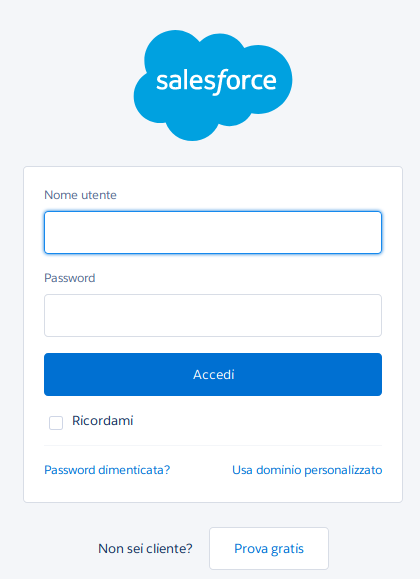
\includegraphics[width=0.4\columnwidth]{login.png} 
    \caption{Schermata di login di Salesforce}
    \label{fig:salesforce-login} 
\end{figure}

\begin{figure}[!h]
    
    \centering
    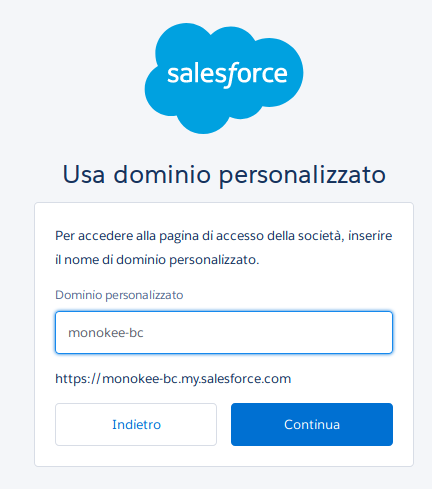
\includegraphics[width=0.4\columnwidth]{dominioLogin.png} 
    \caption{Schermata di scelta dominio}
    \label{fig:salesforce-dom} 
\end{figure}

Indicando il dominio corretto il browser procederà a reindirizzare l'utento presso un apposito sito interno al \emph{back-end} di \emph{Monokee}.

L'inoltro verso il sito scatenerà le seguenti operazioni:
\begin{enumerate}
    \item collegamento verso un canale \gls{websocketg} gestito dal componente \emph{ResultSender} del modulo SP;
    \item attivazione della \emph{web-cam} del computer e cattura di immagini fino all'individuazione di un codice QR compatile con quello generato dall'applicativo mobile IW;
    \item invio tramite comunicazione POST del contenuto del codice QR al modulo SP, la risposta alla POST conterrà un \gls{nonceg} da usare in seguito;
    \item verifica da parte del componente SP delle informazioni di accesso fornite tramite la POST e quindi invio del risultato e del \emph{nonce} tramite il canale \emph{WebSocket}. Il componente SP si occuperà inoltre di comunicare l'esito anche al \emph{back-end} di \emph{Monokee}, il quale si occuperà della generazione della \emph{SAMLResponse}\footnote{La SAMLResponse consiste in \emph{XML} contenente tutte le informazioni necessarie a \emph{Salesforce} per permettere l'accesso. Volendo fare un esempio nel caso di un servizio che richieda \emph{username} e \emph{password}, l'\emph{XML} conterrà questi due dati con l'aggiunta di una serie di firme e informazione utili a garantire la sicurezza del protocolo. Per maggiori dettagli consultare \url{https://www.samltool.com/generic_sso_res.php}.} corrispondente;
    \item inserimento della \emph{SAMLResponse} da parte del \emph{back-end} di \emph{Monokee} all'interno di una \emph{form} presente nel sito;
    \item ricezione da parte del sito dell'esito della verifica tramite il canale \gls{websocketg};
    \item verifica dell'uguaglianza del \emph{nonce} ricevuto dalla POST con quello ricevuto dall'esito della verifica e verifica della positività dell'esito ;
    \item in caso entrambe le verifiche abbiamo riscontro positivo invio tramite POST della \emph{SAMLResponse} al \emph{back-end} di \emph{Salesforce};
    \item reindirizzamento verso l'applicativo \emph{Salesforce}. Ora si è riconosciuti come utenti.
\end{enumerate}

\noindent Qualora una qualsiasi delle precedenti operazioni fallisse o desse esito negativo il sito mostrerà un messaggio di errore a schermo e richiederà la risottimissione del codice QR.
             % Product Prototype
% !TEX encoding = UTF-8
% !TEX TS-program = pdflatex
% !TEX root = ../tesi.tex

%**************************************************************
\chapter{Verifica e validazione}
\label{cap:verifica-validazione}
%************************************************************
\section{Verifica}
Secondo lo stardard ISO/IEC 12207:2008\footcite{ISO:Systems-and-software-engineering} la verifica è un processo di supporto che si occupa di accertarsi che l’esecuzione di un'attività non abbia introdotto errori durante il periodo in esame. 
Ci sono due tipi di verifica: \textbf{statica} e \textbf{dinamica}.
La verifica statica, è estremamente utile in quanto non richiede che il prodotto sia eseguibile, può essere effettuata tramite due tecniche. Queste sono:
\begin{itemize}
    \item ispezione;
    \item analisi a pettine.
\end{itemize}
La verifica dinamica richiede l'esecuzione del codice, questa può essere automatica e ripetibile tramite l'uso di apposite \gls{suitetestg}\glsfirstoccur. I test rappresentano uno dei princiapali esempi di verifica dinamica. Durante le attività di stage è stata adottata una strategia che prevedeva la creazione di test subito dopo la fase di progettazione. Ogni qual volta si prevedeva un componente allora venivano prima redatti i test riguardo a questo e solo in seguito veniva fatta la progettazione in dettaglio. Questo permetteva in maniera immediata di progettare ad alto livello pensando al requisito astratto, ma permetteva anche di progettare in dettaglio con i test.
I test dovevano essere completamente automatizzati ed eseguiti ad ogni commit del codice. 
Per permettere uno sviluppo agevole si è utilizzata una tecnica di gestione del repository detta \emph{branch-pull}.\\
Questa prevedeva che ogni attivita’ di codifica dovesse essere eseguita in un branch creato appositamente allo scopo. Alla fine dell'attività si procedeva con una pull request verso il \emph{branch} principale, questa veniva accettata se e solo se i test passavano completamente. \\

Le attivatà di verifica erano mirate al raggiungimento dei seguenti obiettivi: 
\begin{itemize}
    \item rilevazione di errori di codifica;
    \item rilevazione di modifiche nei requisiti;
    \item rilevazione di modifiche nella progettazione;
    \item individuazione dell’uso di componenti di cui non si conosce chiaramente il comportamento;
    \item rilevazione di integrazioni tra componenti non adatte.
\end{itemize}
\medskip
Un punto critico è stato quello di trovare un giusto quantitativo di test da produrre. Esagerando avremmo rischiato di superare la scadenza inerenti alle attività di codifica.
Abbiamo quindi deciso di produrre almeno un test per metodo ed un test per classe. 
Data l’elevata difficoltà nel prevedere test di integrazione e di sistema abbiamo deciso di farli solo in caso ci fosse stato tempo. 
L'uso di queste tecniche ha inoltre permesso di avere una certa libertà nelle modifiche a codice già integrato nel sistema, in quanto ha fornito almeno in parte anche dei test di regressione. 

Lo svolgimento di questo processo ha permesso di ottenere varie metriche quali:
\begin{itemize}
    \item test coverage;
    \item percentuale di test passati;
    \item copertura dei requisiti.
\end{itemize}

\subsection{Attività di verifica statica}
I componenti basandosi sullo stesso linguaggio hanno condiviso le procedure per la verifica statica. Il principale strumento di utilizzato è stato il linter \emph{SonarLint}. Questo strumento ha permesso di mantenere lo stesso stile di scrittura in ogni parte del progetto, inoltre aveva funzioni che permettevano l'individuazine di potenziali errori logici e cattive pratiche. 
Inoltre sono state utilizzate numerose funzionalità presenti in \emph{Visul Studio} che permettevano refactoring automatici del codice e strumenti di analisi statica.

\subsection{Realizzazione dei test}
Entrambi i componente codificati durante le 320 ore di stage condividevano lo stesso linguaggio di programmazione, ma utilizzavano \gls{frameworkg} diversi. Nonostante molte librerie fossero in comune questo non lo era per i framework di test. Il test per il componente SP sono stati codificati usando \emph{MSTest}, mentre quelli per il componente IW hanno usato \emph{Xamarin.UITest}

Particolare difficoltà è stata riscontrata nei test di integrazione del componente SP. Questo infatti lavora in stretto conttato con l'applicativo Monokee e con i componenti IW e ITF. Data l'elevata mutabilità dell'applicativo Monokee si è deciso di realizzare doppie versioni di ogni test; la prima prevedento l'uso di \emph{mock}, la seconda  effettuando una reale comunicazione con i componenti precedentemente citati. Questo ha permesso una più semplice localizzazione dei problemi.

Il componente IW è un'applicazione mobile le cui interazioni con elementi esterni sono di natura occasionale e al solo fine di ottenere informazioni verificabili. Per questa ragione si è ritenuto di non usare dei \emph{mock}, ma di prevedere direttamente test che comunicassero con gli elementi esterni.


\section{Validazione}
La validazione si occupa di accertarsi che il prodotto sviluppato sia quello realmente desiderato. In genere è fatta a prodotto finito ed è utile al fine di capire se il prodotto soddisfa il cliente e gli utenti finali. La principale attività di validazione è stata svolta l'ultima settimana di lavoro tramite prove e dimostrazioni del prodotto. In quei giorni si è verificato con la presenza del tutor aziendale la corretta implementazione dei requisiti dedotti durante le prime fasi di analisi.

L'esito, seppur non vedendo la totalità dei requisiti soddisfatti, è stato soddisfacente. Si preme di tenere conto che molto requisiti sono stati ritenuti di importanza accessoria dall'azienda e sostituiti con altre funzionalità non previste inizialmente.


\subsection{Validazione requisiti componente IW}
In tabella \ref{tab:validazione-iw} si mostra lo stato di validazione di ogni requisiti del componente IW, questi possono essere:
\begin{itemize}
    \item implementati: se il requisito è stato implementato correttamente e riconosciuto come tale dal tutor aziendale;
    \item non implementato: se il requisito non è stato inserito nel progetto o non funziona come aspettato;
    \item cancellato: se il requisito è stato ritenuto non più di interesse o non più compatibile con il progetto da parte del tutor aziendali.
\end{itemize}

\begin{center}
    \begin{longtable}{|p{3cm}|p{3cm}|}%
    \caption{Tabella validazione IW}
    \label{tab:validazione-iw}
    \endfirsthead
    \endhead
    \hline
    \textbf{Codice}  & \textbf{Stato}\\
    \hline
    R[F][C]0001    & non implementato  \\
    \hline
    R[F][C]0002   & non implementato  \\
    \hline
    R[F][C]0003    & non implementato  \\
    \hline
    R[F][C]0004    & non implementato \\
    \hline
    R[F][M]0005    & annullato  \\
    \hline
    R[F][M]0006    & implementato  \\
    \hline
    R[F][M]0007    & annullato \\
    \hline
    R[F][M]0008    & implementato  \\
    \hline
    R[F][M]0009    & annullato  \\
    \hline
    R[F][M]0010    & annullato  \\
    \hline
    R[F][M]0011    & annullato  \\
    \hline
    R[F][M]0012    &  implementato\\
    \hline
    R[F][M] 0013    &  implementato\\
    \hline
    R[F][M] 0014    &  implementato  \\
    \hline
    R[F][M] 0015    &  implementato  \\
    \hline
    R[F][M] 0016    &  implementato  \\
    \hline
    R[F][M] 0017    &  implementato  \\
    \hline
    R[F][M] 0018    &  implementato  \\
    \hline
    R[F][M] 0019    &  implementato  \\
    \hline
    R[F][M] 0020    &  implementato \\
    \hline
    R[F][M] 0021    &  implementato \\
    \hline
    R[F][M] 0022    &  implementato \\
    \hline
    R[F][M] 0023    &  implementato \\
    \hline
    R[F][M] 0024    &  implementato  \\
    \hline
    R[F][M] 0025    &  implementato  \\
    \hline
    R[F][S] 0026    &  non implementato  \\
    \hline
    R[V][M] 0027    & implementato  \\
    \hline
    R[V][M] 0028    & implementato  \\
    \hline
    R[V][M] 0029    & implementato  \\
    \hline
    R[V][M] 0030    & implementato  \\
    \hline
    R[V][M] 0031    & implementato  \\
    \hline
    R[Q][S] 0032    & implementato  \\
    \hline
    R[Q][S] 0033    & implementato  \\
    \hline
    R[Q][S] 0034    & implementato  \\
    \hline
    R[Q][S] 0035    & implementato  \\
    \hline
    R[Q][C] 0036    & implementato  \\
    \hline
    \end{longtable}
    \end{center}

I requisiti:
\begin{itemize}
    \item R[F][C]001;
    \item R[F][C]002;
    \item R[F][C]003;
    \item R[F][C]004
\end{itemize}
non sono stati implementati in quanto questi sono stati pensati in un'ottica che prevedeva la distribuzione al grande pubblico dell'applicazione. Questi requisiti sono stati quindi ritenuti dal tutor aziendale non importanti e rimanabili a successivi rilasci.

I requisiti: 
\begin{itemize}
    \item R[F][M]0005; 
    \item R[F][M]0007; 
    \item R[F][M]0009; 
    \item R[F][M]0010; 
    \item R[F][M]0011 
\end{itemize}
sono stati cancellati in quanto si è deciso che le funzionalità che proponevano non dovessero essere offerte dall'applicazione, ma dal portale attualmente esistente di Monokee.

Il requisto R[F][S] 0026 non è stato implementato in quanto prevedeva una continua comunicazione con l'ITF e l'uso di notifiche push. Si è ritenuto, in accordo con il tutor aziendale, che lo sforzo sarebbe stato eccessivo rispletto al valore che avrebbe apportato la funzionalità. Per questo si è deciso di rimandare lo sviluppo a successive versioni dell'applicativo.

\subsection{Validazione requisiti componente SP}
In tabella \ref{tab:validazione-sp} si mostra lo stato di validazione di ogni requisiti del componente SP, questi possono essere:
\begin{itemize}
    \item implementati: se il requisito è stato implementato correttamente e riconosciuto come tale dal tutor aziendale;
    \item non implementato: se il requisito non è stato inserito nel progetto o non funziona come aspettato;
    \item cancellato: se il requisito è stato ritenuto non più di interesse o non più compatibile con il progetto da parte del tutor aziendali.
\end{itemize}
\begin{center}
    \begin{longtable}{|p{3cm}|p{3cm}|}%
    \caption{Tabella di validazione SP}
    \label{tab:validazione-sp}
    \endfirsthead
    \endhead
    \hline
    \textbf{Codice}  & \textbf{Stato}\\
    \hline
    R[F][M]0001    & implementato  \\
    \hline
    R[F][M]0002    & implementato  \\
    \hline
    R[F][M]0003    & implementato  \\
    \hline
    R[F][M]0004    & implementato  \\
    \hline
    R[F][M]0005    & implementato  \\
    \hline
    R[F][M]0006    & implementato  \\
    \hline
    R[F][M]0007    & implementato  \\
    \hline
    R[F][M]0008    & implementato  \\
    \hline
    R[F][M]0009    & implementato  \\
    \hline
    R[F][M]0010    & implementato  \\
    \hline
    R[F][M]0011    & implementato  \\
    \hline
    R[F][M]0012    & implementato  \\
    \hline
    R[F][M]0013    & implementato  \\
    \hline
    R[F][M]0014    & implementato  \\
    \hline
    R[F][M]0015    & implementato  \\
    \hline
    R[F][M]0016    & implementato  \\
    \hline
    R[F][M]0017    & implementato  \\
    \hline
    R[V][M] 0018    & implementato  \\
    \hline
    R[V][M] 0019    & implementato  \\
    \hline
    R[V][M] 0020    & implementato  \\
    \hline
    R[V][M] 0021    & implementato  \\
    \hline
    R[V][C] 0022    & implementato  \\
    \hline
    R[Q][S] 0023    & implementato  \\
    \hline
    R[Q][S] 0024    & implementato  \\
    \hline
    R[Q][S] 0025    & implementato  \\
    \hline
    R[Q][S] 0026    & implementato  \\
    \hline
    R[Q][C] 0027    & implementato  \\
    \hline
    R[Q][C] 0028    & implementato  \\
    \hline
    \end{longtable}
    \end{center}%

I requistiti relativi al componente SP sono stati complementamente implementati e validati dal tutor aziendale.             % Product Design Freeze e SOP
% !TEX encoding = UTF-8
% !TEX TS-program = pdflatex
% !TEX root = ../tesi.tex

%**************************************************************
\chapter{Conclusioni}
\label{cap:conclusioni}
%**************************************************************

%**************************************************************

%**************************************************************
%**************************************************************
\section{Conoscenze acquisite}
Il progetto si colloca in un servizio più grande qual è \emph{Monokee}, motivo per cui si è reso neccessario uno sviluppo che tenesse conto di differenti progetti esistenti, di cui alcuni già in produzione ed altri in via di sviluppo (i.e. il componente ITF). Questo mi ha permesso di lavorare in un contesto che richiedeva di interagire costantemente con altri team e quindi operare in maniera controllata, disciplinata e coordinata. È stato quindi fondamentale acquisire pratiche di ingegneria del software e attuare correttamente le pratiche aziendali (queste si basavano su \gls{scrumg}).

Il piano di lavoro prevedeva lo sviluppo di due componenti: l'\textbf{Identity Wallet} (IW) e il \textbf{Service Provider} (SP). Questi sono da considerarsi due prodotti completamente separati tra di loro che concorrono, in aggiunta al componente ITF (sviluppato da un altro stagista), a fornire un unico servizio. Sono applicativi di natura diversa; il primo un'applicazione mobile, il secondo un'applicazione server, che, di conseguenza hanno richiesto conoscenze diverse dandomi la possibilità di acquisire più competenze.

Di seguito viene proposta una lista delle principali competente acquisite durante le attività di stage e non precedentemente conosciute:
\begin{itemize}
    \item apprendimento del linguaggio C\#;
    \item sviluppo di interfacce touch in Xamarin;
    \item creazione di servizi RESTful;
    \item apprendimento dell'uso di WebSocket;
    \item uso del framework .NET Core;
    \item uso del framework  Asp.NET;
    \item progettazione di un'architettura Event Driven;
    \item uso di RabbitMQ e MassTransit;
    \item integrazione con SAML.
\end{itemize}

Inoltre ho avuto l'opportunità di approfondire e mettere in pratica alcune delle conoscenze acquisite durante il corso di laurea triennale; tra queste riporto:
\begin{itemize}
    \item metodologie e pratiche di ingegneria del software;
    \item uso di HTML5 e javascript;
    \item uso di lambda funzioni (\emph{arrow function}) in un linguaggio imperativo;
    \item ideazione e codifica di test.
\end{itemize}


%**************************************************************
\section{Valutazione personale}
Il periodo di stage svolto presso \emph{IvoxIT}, a conclusione del mio percorso di studi, è stato fondamentale per approfondire ed ampliare le conoscenze in mio possesso; tra queste, alcune di carattere tecnologico, altre di carattere metodologico e, a tal proposito, indispensabili sono stati i vari corsi di programmazione e il corso di ingegneria del software. Oltre a ciò, ho avuto modo di sviluppare nuove competenze, apprendere tecnologie e sistemi che mi torneranno utili nel futuro. 

In questi mesi ho avuto l'occasione di lavorare ed inserirmi in un gruppo estremamente affiatato e coeso con cui ho avuto la possibilità di confrontarmi al fine di rendere il mio progetto veramente utile agli scopi aziendali. Ho potuto fare affidamento su persone con grande esperienza e capacità, e questo mi ha permesso di rendere più veloci e di maggior qualità le attività di analisi, progettazione e codifica. Ho inoltre aprezzato come i miei colleghi, anche se non a conoscenza della particolare tecnologia, disponessero di attitudine e metodo, cosa che permetteva loro un rapido apprendimento e la capacità di fornirmi un aiuto concreto. I rapporti instaurati non sono stati solo di natura prettamente didattica e lavorativa, ma anche di amicizia e stima reciproca. Penso di aver avuto modo di lavorare e consultarmi con persone di elavata caratura sia lavorativa che personale. 

Il progetto è stato sviluppato nei tempi previsti e nonostante le grandi fluttuazioni in termini di requisiti e di aspetti progettuali che questo ha avuto, il risultato è stato soddisfacente. Tuttavia il prodotto finale ha fatto emergere le innumerevoli problematiche legate all'uso della tecnologia \gls{blockchaing}. Una blockchain permissionless ha infatti tempi di elaborazione difficilmente accettabili da un utente medio. Nel corso della settimana finale si sono svolti test di prestazione sulla rete \gls{ropsteng} che hanno mostrato come anche per le chiamate più semplici, che richiedevano almeno un'operazione di scrittura, ci fosse un tempo minimo di attesa pari a 30s. Ciò nonostante, a seguito di operazioni di ottimizzazione, siamo riusciuti ad eseguire le chiamate alla blockchain in parallelo arrivando ad un tempo totale necessario al login pari a 32s. Tale lentezza è dovuta alla necessaria \emph{proof of interest}, che in una rete di questo tipo consiste nel risolvere un problema matematico (\emph{proof of work}) di difficoltà variabile in base alle esigenza.  
In conclusione, ritengo che i vantaggi legati all'uso di una blockchain siano:
\begin{itemize}
    \item affidabilità;
    \item disponibilità;
    \item eliminazione di intermediari
\end{itemize} 
non sufficienti a giustificare nella maggioranza dei casi una durata così elevata per una semplice operazione di login.
Inoltre, uno degli obiettivi principali dell'azienda era quello di inglobale tale sistema in quello attuale. Ciò ha portato ad una serie di scelte che hanno annulato alcune fondamentali caratteristiche della blockchain. Il componente SP rappresenta un sistema centralizzato e quindi un grosso \emph{point of failure} che mina l'elevata disponibilità tipica della blockchain (in quanto sistema distribuito). Un altro punto critico riguarda invece l'uso di account gestiti direttamente dall'azienda per tutte le operazioni. Lo scopo era quello di rendere gli utenti liberi dal dover gestire i propri account, ma in una previsione di alto utilizzo del sistema renderebbe complicato per una persona verificare le transazioni e quindi farebbe venir meno la carrateristica di fiducia tipica delle blockchain, in quanto la mole di transazioni renderebbe difficile l'identificazione delle proprie.

In conclusione da questa esperienza ho appreso che una buona preparazione sia in termini di conoscenze che di competenze, è sì necessaria, ma non preclusiva ai fini del lavoro. È invece indispensabile l'attitudine e il pensiero analitico, il quale permette di trovare la soluzione più adatta di fronte ai problemi e affrontare al meglio le varie difficoltà 

Infine, avendo avuto uno spaccato reale di quello che il mio percorso di studi si può riversare a livello professionale, ho avuto maggiore chiarezza dei possibili ambiti occupazionali e di conseguenza ho potuto fare delle considerazioni, rafforzando così la mia convinzione nel proseguire con gli studi magistrali e maturando prospettive più precise.


\epigraph{La conclusione è il punto dove ti sei stufato di pensare.}{Arthur Bloch}             % Conclusioni
\appendix                               
% !TEX encoding = UTF-8
% !TEX TS-program = pdflatex
% !TEX root = ../tesi.tex

%**************************************************************
\chapter{Appendice A}
\section{Strumenti utili per lavorare su Ethereum}
\label{cap:str_eth}
Di seguito una breve descrizione di alcuni strumenti utili per lavorare su \emph{Ethereum}.
\begin{itemize}
    \item \textbf{Truffle}: è una suite di development e testing. Permette di compilare, buildare ed effettuare la migrazione degli SmartContract. Inoltre ha funzioni di debugging e di scripting. La suite offre la possibilità di effettuare test degli SmartContract sia in Javascript (con l’utilizzo di Chai), sia in Solidity. Si riporta di seguito il sito del progetto: \cite{site:truffle}.
    \item \textbf{Ganache}: è uno strumento rapido che permette di creare e mantenere in locale una rete blockchain Ethereum personale. Può essere usata per eseguire test, eseguire comandi e per operazioni di controllo dello stato mentre il codice esegue. Si riporta di seguito il sito del progetto: \cite{site:ganache}.
    \item \textbf{Mist}: è un browser sviluppato direttamente dal team Ethereum in grado di operare transazioni direttamente nella blockchain senza la necessità di possedere un intero nodo. È estremamente immaturo e non utilizzabile in produzione. Si riporta di seguito il sito del progetto: \cite{site:mist}.
    \item \textbf{Parity}: è un client Ethereum che permette di operare sulla rete senza necessità di possedere un intero nodo. Questa soluzione a differenza di Mist dovrebbe risultare più facilmente integrabile nel prodotto senza che l’utente ne abbi consapevolezza. Si riporta di seguito il sito del progetto: \cite{site:parity} .
    \item \textbf{Metamask}: è uno plugin disponibile per i browser Chrome, Firefox, e Opera. Permette di interfacciarsi alla rete Ethereum senza la necessità di eseguire in intero nodo della rete. Il plugin include un wallet con cui l’utente può inserire il proprio account tramite la chiave privata. Una volta inserito l’account il plugin farà da tramite tra l’applicazione e la rete.
    Metamask è utilizzato dalla maggioranza delle applicazioni Ethereum presenti on line, questo però rappresenterebbe un componente esterno compatibile con pochi browser desktop. Si riporta di seguito il sito del progetto: \cite{site:metamask} .
    \item \textbf{Status}: è un progetto che propone una serie di \gls{apig} che permettono di sviluppare un’applicazione mobile nativa operante direttamente su blockchain senza la necessità di possedere un intero nodo. Il sito del progetto propone una serie di applicazioni che utilizzano Status. Tuttavia nessuna di queste applicazioni risulta attualmente rilasciate in nessuno store. Status risulta in early access ed è disponibile per Android e iOS. Il sito del progetto è il seguente: \cite{site:status}.
    \item \textbf{Microsoft Azure}: “Ethereum Blockchain as a Service” è un servizio fornito da Microsoft e ConsenSys che permette di sviluppare a basso costo in un ambiente di dev/test/produzione. Permette di creare reti private, pubbliche e di consorzio. Queste reti saranno poi accessibili attraverso la rete privata Azure. Questa tecnologia rende facile l’integrazione con Cortana Analytics, Power BI, Azure Active Directory, O365 e CRMOL.
\end{itemize}
%**************************************************************





             % Appendice A

%**************************************************************
% Materiale finale
%**************************************************************
\backmatter
\printglossaries
% !TEX encoding = UTF-8
% !TEX TS-program = pdflatex
% !TEX root = ../tesi.tex

%**************************************************************
% Bibliografia
%**************************************************************

\cleardoublepage
\chapter{Bibliografia}

\nocite{*}
% Stampa i riferimenti bibliografici
\printbibliography[heading=subbibliography,title={Riferimenti bibliografici},type=book]

% Stampa i siti web consultati
\printbibliography[heading=subbibliography,title={Siti web consultati},type=online]


\end{document}
